\documentclass[a4paper,12pt]{book}
\usepackage{geometry}
\geometry{
a4paper,
total={170mm,257mm},
left=20mm,
top=20mm,
}
\usepackage[utf8]{inputenc}
\usepackage{titletoc}
\usepackage[brazil]{babel}
\usepackage{graphicx}
\usepackage{sidecap}
\usepackage{csquotes}
\setcounter{secnumdepth}{5}
\setcounter{tocdepth}{3}
\usepackage{parskip}
\usepackage{float}
\usepackage{wrapfig, booktabs, tabularx}
\usepackage[version=4]{mhchem}
%\usepackage{quattrocento}
\usepackage[sfdefault,light]{FiraSans} %% option 'sfdefault' activates Fira Sans as the default text font
\usepackage[T1]{fontenc}
\renewcommand*\oldstylenums[1]{{\firaoldstyle #1}}
\usepackage{chemfig}
\usepackage{xymtexpdf}
\usepackage[backend=biber]{biblatex}
\usepackage[Sonny]{fncychap}
\usepackage{adjustbox}
\usepackage{caption}
%\usepackage{showframe}
\usepackage{array}
\usepackage{longtable}
\usepackage{multirow}

\usepackage{nomencl}
\makenomenclature

\newcommand{\source}[1]{\caption*{Fonte: {#1}} }

\usepackage{copyrightbox}
\addbibresource{livro.bib}

%% INSERT YOUR PACKAGES HERE
\usepackage[accsupp]{axessibility}  % improves PDF readability for those with disabilities.
\usepackage{lipsum}
\usepackage{tcolorbox}
\usepackage{listings}
\usepackage{hyperref}
\hypersetup{
	colorlinks=true,
	linkcolor=blue,
	filecolor=magenta,      
	urlcolor=cyan,
	pdftitle={Química Orgância Básica},
	pdfpagemode=FullScreen,
}
\urlstyle{same}
\usepackage{makeidx}

\begin{document}

\author{JHGB / ACM}
\title{Química Orgânica Básica}
\date{Dezembro 2023}

\frontmatter
\maketitle
\tableofcontents
\listoffigures 
\listoftables 


\mainmatter

\part{Como tudo começou}
\chapter{O início de todas as partículas e elementos}
O autor deste livro sempre tentou ensinar a seus alunos a origem primária de cada item que ensina, como por exemplo a Equação de Estado de Gases Ideais, ou então a viscosidade de fluidos. Porém, quando se trata de elementos químicos a situação fica um pouco mais complicada porque os elementos químicos, esses pequenos blocos construtivos, não foram produzidos neste planeta por uma razão simples: não há energia suficiente por aqui para uma tarefa tão grande quanto a fusão de núcleos menores para formar átomos maiores, ne escala de quantidade necessária para formar um planeta como a Terra.

Temos neste momento ao menos duas perguntas ecoando na cabeça da pessoa que lê este livro bem agora: (a) por que é necessária tanta energia e (b) onde e como tais átomos foram criados?

Analisemos o elemento químico mais simples existente e construiremos as respostas. O Hidrogênio é composto por um próton, um elétron e ainda nenhum, um ou dois nêutrons, dependendo do isótopo \footnote{Isótopos são conjuntos de átomos com o mesmo número atômico, diferindo uns dos outros pela quantidade de nêutrons de cada um deles} analisado. O segundo elemento mais simples, depois do Hidrogênio é conhecido como Hélio e possui dois prótons em seu núcleo. Parece simples, não é? Porém, não é tão simples como parece.

Se considerarmos o Big Bang como o início de tudo que existe no universo conhecido, sabemos que as primeiras partículas a se formarem foram aquelas que chamamos de \textbf{fundamentais} \cite{griffiths2020introduction} e entre elas citamos os quarks, elétrons, fótons e glúons, como pode ser visto na figura \ref{fig:particulaselementares}

\begin{figure}[h]
	\centering
	\caption{Modelo Padrão de partículas elementares}
	\vspace{0.25cm}
	\label{fig:particulaselementares}
	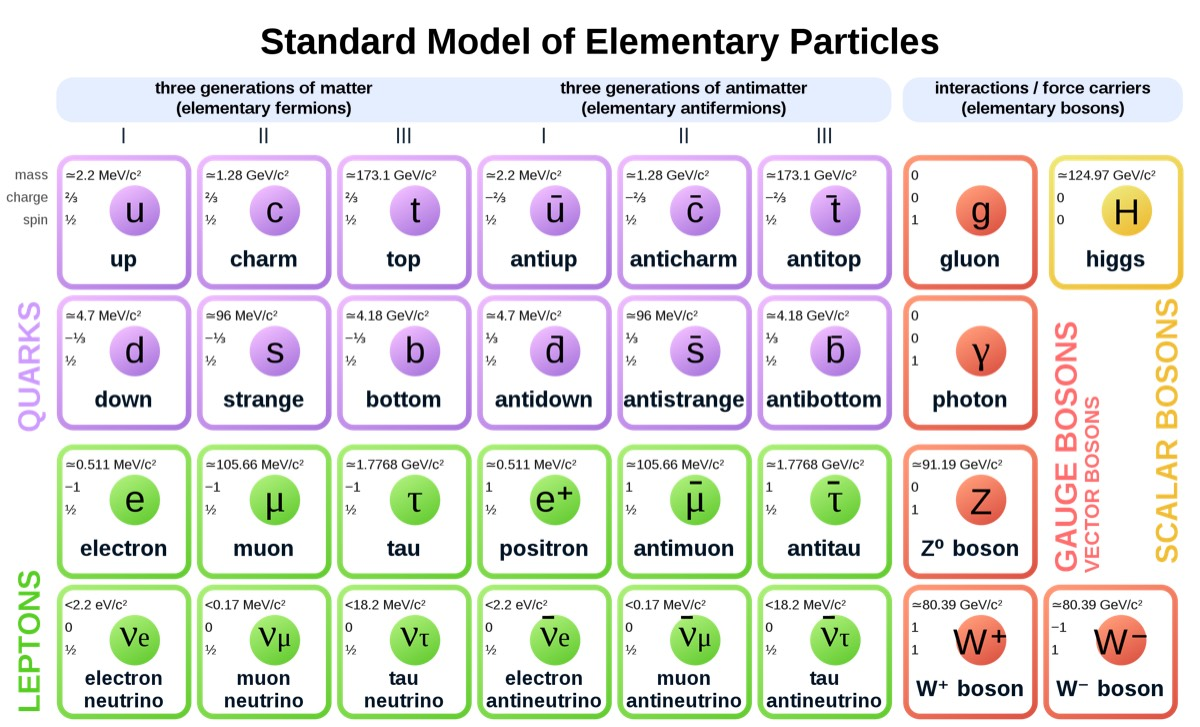
\includegraphics[width=1\linewidth]{imagens/boson2.jpg}
\end{figure}

A descrição completa da figura \ref{fig:particulaselementares} está além do escopo primário deste livro, mas podemos analisar, sem grandes dificuldades, a composição detalhada de um próton, pois você deve lembrar-se que seis desses prótons formam o núcleo do magnífico carbono.

Não é tão complicado e siga o fio para entender claramente. Sabemos que o próton possui carga positiva com valor 1,6{$\cdot$}10{$^{-19}$} C \footnote{C é a unidade de carga chamada Coulomb} e massa aproximada de 1 u. Estudos na área da Física de Alta Energia mostraram que o próton é formado por três quarks: dois quarks up e um quark down, unidos por um bóson chamado \textbf{glúon} Seguindo os dados presentes na figura \ref{fig:particulaselementares}, cada quark up possui carga +2/3 e cada quark down possui carga -1/3. A soma simples dessas cargas resulta em 3/3, ou seja, 1. 

A manutenção desse sistema todo que mantém o próton íntegro é mediada pela Força Nuclear Forte, uma das forças elementares da Natureza e também a mais forte delas, embora atue apenas na escala nuclear.

De modo semelhante e com resultados dos mesmos estudos, um nêutron (com carga zero) é formado um quark up e dois quarks down. A soma dessas cargas resulta em zero!

Muito bem! Já sabemos como se organizam as três partículas de mais fácil compreensão em átomos: prótons, nêutrons e elétrons. Mas precisamos entender como são produzidos átomos maiores, o que nos deixa com outra pergunta um tanto séria: conhecendo o Princípio de Repulsão das Cargas Elétricas, como é possível manter, por exemplo, dois prótons em um núcleo atômico? A resposta possui duas partes:

\begin{enumerate}
	\item \textbf{A presença de nêutrons}. Sabemos que estas partículas são formadas por um próton e um elétron, mantidos unidos por uma entidade sem massa nem carga chamada \textbf{neutrino}. Uma das funções dos nêutrons no núcleo atômico é justamente afastar um pouco os prótons de outros prótons, como forma de diminuir a repulsão elétrica causada pela proximidade de partículas de mesma carga colocadas em uma distância tão pequena como as verificadas em escala nuclear.
	\item \textbf{A Força Nuclear Forte}: A força nuclear forte é uma das quatro forças fundamentais da natureza, responsável pela coesão entre os núcleos atômicos. Ela é responsável por manter os prótons e nêutrons unidos, apesar da repulsão eletromagnética entre os prótons, que são carregados positivamente. A força nuclear forte é muito mais forte que a força eletromagnética, sendo cerca de 100 vezes mais forte. No entanto, ela tem um alcance muito curto, de apenas cerca de 10-15 metros. Isso significa que ela só é significativa em distâncias muito pequenas, como no interior do núcleo atômico.
	
	A força nuclear forte é mediada por partículas chamadas glúons. Os glúons são partículas elementares sem massa, que carregam a carga de cor. A força nuclear forte é responsável por ligar os quarks, que são as partículas elementares que compõem os prótons e nêutrons. A força nuclear forte é fundamental para a existência da matéria como a conhecemos. Ela é responsável pela formação dos átomos, das moléculas e das estrelas. Sem a força nuclear forte, o universo seria um lugar muito diferente, com átomos muito instáveis e sem a possibilidade de formar estruturas complexas.
\end{enumerate}

Para entendermos como essas partículas nucleares foram criadas, precisamos compreender que partículas maiores são sempre formadas a partir da junção ou fusão de partículas menores, e tal operação requer energia em quantidades incrivelmente altas, obtidas apenas em condições experimentais raras e caras, ou ainda em estrelas, principalmente aquelas presentes na chamada "Sequência Principal".

\section{Ciclo de Vida Estelar}\index{Ciclo de vida estelar}

Todas as estrelas conhecidas transitam pela chamada "Sequência Principal", onde o núcleo estelar possui as condições de temperatura e pressão capazes de fundir Hidrogênio em Hélio, exigindo temperatura próxima de 100 milhões K. Em função de sua massa, nosso Sol queimará todo seu Hidrogênio em Hélio durante um intervalo de tempo bastante grande, por volta de 4 ou 5 bilhões de anos. Depois de esgotar seu combustível, o Sol sofrerá uma transformação radical e converte-se-á em uma gigante vermelha, com capacidade nuclear para produzir Carbono e Oxigênio. Porém, para tanto, seu tamanho aumentará sobremaneira que inviabilizará a vida na Terra \footnote{O Sol crescerá de tamanho em uma escala tão intensa que destruirá nosso planetinha azul}. Veja na figura \ref{fig:HR} a correlação entre cor e magnitude das estrelas.

\begin{figure}[h]
	\centering
	\caption{Diagrama de Hertzsprung-Russell}
	\vspace{0.25cm}
	\label{fig:HR}
	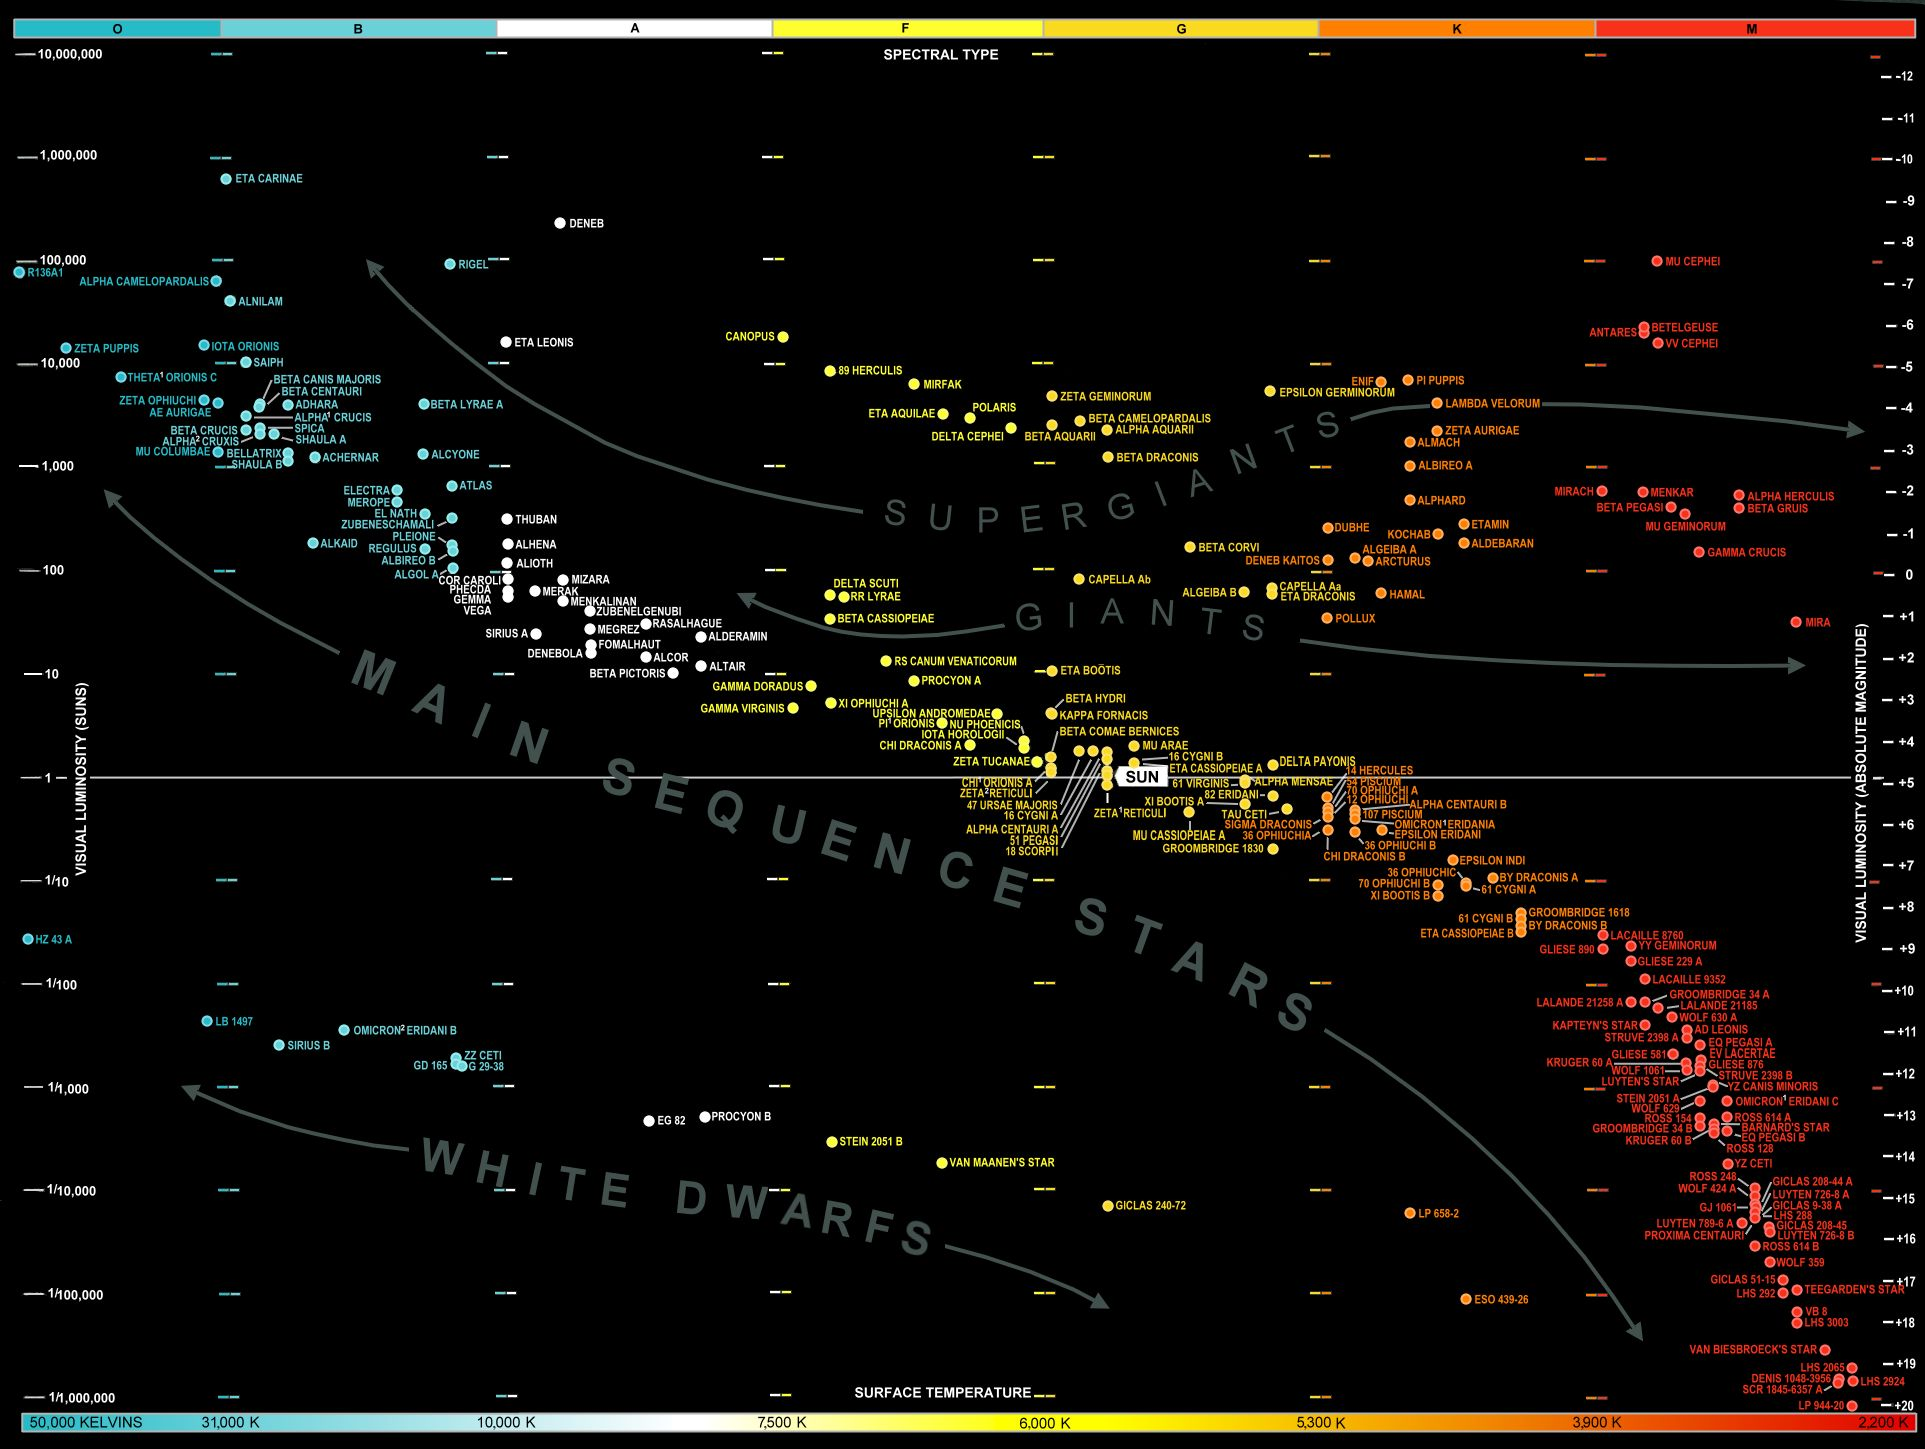
\includegraphics[width=1\linewidth]{imagens/diagrama-hr-completo.jpg}
\end{figure}

O Diagrama HR, ou Diagrama de Hertzsprung-Russell \cite{HR}, é um gráfico que mostra a relação entre a luminosidade e a temperatura de superfície de uma estrela. A luminosidade é uma medida da quantidade de energia que uma estrela emite, enquanto a temperatura de superfície é uma medida da temperatura da camada externa da estrela.

É um dos diagramas mais importantes da astronomia, pois fornece informações valiosas sobre a evolução das estrelas. As estrelas são classificadas em tipos espectrais, que são uma medida da temperatura de superfície da estrela. Estrelas de tipo espectral O são as mais quentes, enquanto estrelas de tipo espectral M são as mais frias. Pode ser dividido em várias regiões, cada uma das quais representa um estágio diferente da evolução estelar. A sequência principal é a região mais larga do Diagrama HR e contém a maioria das estrelas da nossa galáxia. As estrelas da sequência principal estão gerando energia através da fusão de hidrogênio no núcleo.

As estrelas quentes e brilhantes, como as estrelas de tipo O e B, estão localizadas no canto superior esquerdo do Diagrama HR. Essas estrelas são muito jovens e estão consumindo seu hidrogênio muito rapidamente. Elas viverão por apenas alguns milhões de anos. As estrelas frias e fracas, como as estrelas de tipo M, estão localizadas no canto inferior direito do Diagrama HR. Essas estrelas são muito velhas e estão consumindo seu hidrogênio muito lentamente. Elas viverão por bilhões de anos. O Diagrama HR também pode ser usado para identificar estrelas que estão passando por eventos importantes em sua evolução. Por exemplo, as estrelas gigantes vermelhas estão localizadas no canto superior direito do Diagrama HR. Essas estrelas estão deixando a sequência principal e estão expandindo e esfriando.

A produção de Carbono, em estrelas mais massivas que o Sol, envolve temperaturas bem mais altas que em nosso Sol e ocorre em camadas mais profundas na estrela e o caminho em direção ao centro aumenta a temperatura e pressão cada vez mais, possibilitando a nucleossíntese de outros elementos químicos, até o Ferro. Elementos mais pesados que o Ferro são produzidos em eventos extremos, como a explosão de supernovas, estrelas muito massivas que esgotam seu combustível então explodem. Esse evento extremo espalha elementos químicos produzidos na explosão e, eventualmente, enriquece nuvens de gases e poeira onde o Sol e Terra se formaram. Assim, os elementos que aqui existem são originários da destruição de outras estrelas.

Legal, mas e o Carbono?

\chapter{Nucleossíntese do Carbono}
A vida no planeta Terra é baseada no elemento químico carbono e por tal razão iniciamos nossa jornada a partir do ponto zero: como os átomos de carbono são produzidos em processos estelares. Para que você aí tenha uma ideia da dimensão energética envolvida, a temperatura necessária atinge, aproximadamente, 100.000.000 K. Isso mesmo: cem milhões!

É um consenso que átomos de carbono formaram-se, assim como outros elementos, através de violentíssimos choques causados por cenários que beiram o inimaginável, como a quase inacreditável temperatura citada logo acima. Naturalmente, os pesquisadores que desenvolveram - e comprovaram - essas ideias foram laureados com o Prêmio Nobel de Física em 1983 \footnote{Veja mais em https://www.nobelprize.org/prizes/physics/1983/summary/}, quase 30 anos após os estudos iniciais.

Estrelas com capacidade energética suficiente conseguem "fundir carbono" \index{Nucleossíntese do carbono}, usando uma terminologia muito frequente na área astronômica. As mais recentes concepções sobre a nucleossíntese do Carbono envolvem um processo conhecido como "Triplo Alfa". A expressão "fundir carbono" significa um conjunto de reações nucleares que parte de átomos mais leves, como Hélio ou Berílio, para formar o núcleo do carbono, por meio da fusão nuclear. Este método exige muita energia, e a produção de elementos mais pesados que o carbono requer ainda mais energia.

Como assim?

\section{O Processo Triplo Alfa}

Sabemos há um bom tempo que o núcleo do átomo de Carbono é composto por seis prótons e seis nêutrons, com total de doze partículas. Repare que o nome do processo relaciona-se com uma partícula radioativa conhecida como radiação (ou partícula) alfa, que possui dois prótons e dois nêutrons, mas sem seus elétrons, o equivalente ao núcleo do átomo de Hélio. Se você unir três dessas partículas, obterá o núcleo do carbono. Interessante, não é? É o chamado Processo Triplo Alfa \index{Processo Triplo Alfa} \cite{TA}.

Analise a figura \ref{fig:triploalfa} seguinte para melhor compreensão do processo, embora exibido de modo bem simplificado.

\begin{figure}[h]
	\centering
	\caption{O Processo Triplo Alfa}
	\vspace{0.25cm}
	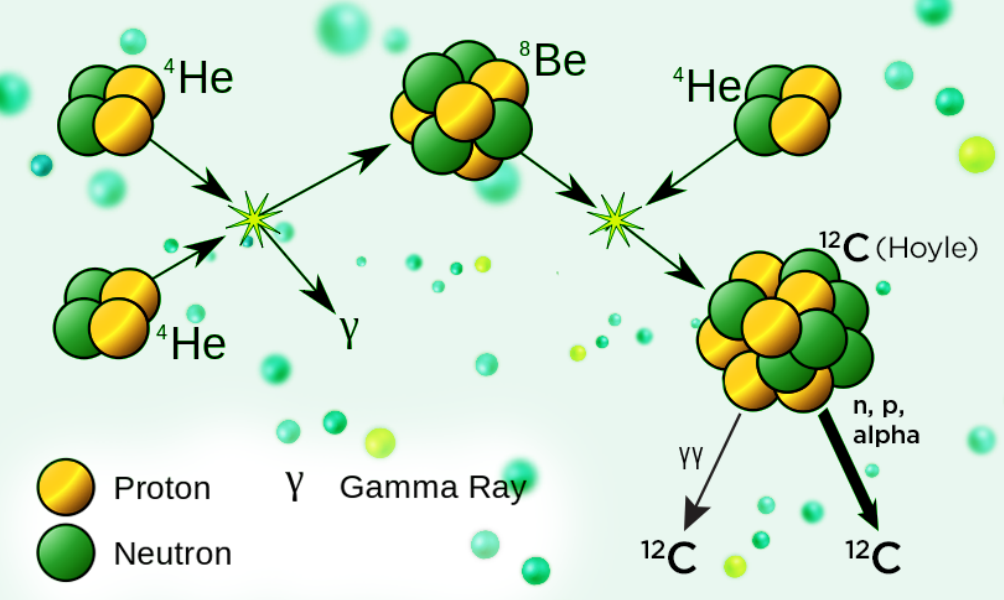
\includegraphics[width=0.75\linewidth]{imagens/figura 2.png} 
	\label{fig:triploalfa}
\end{figure}

O processo triplo alfa é uma reação nuclear de fusão que converte três núcleos de hélio (partículas alfa) em um núcleo de carbono. Este processo é responsável pela produção de carbono no universo, e é um dos processos mais importantes na nucleossíntese estelar.

O processo triplo alfa ocorre em temperaturas muito altas, acima de 100 milhões de kelvin. Essas temperaturas são encontradas no núcleo das estrelas, onde o hidrogênio é fundido em hélio e ocorre em duas etapas:

\begin{enumerate}
	\item \textbf{Berílio-8}: Duas partículas alfa se fundem para formar um núcleo de berílio-8. O berílio-8 é um núcleo instável, que se decompõe em duas partículas alfa em cerca de $10^{-16}$ segundos.
	\item \textbf{Carbono-12}: Uma partícula alfa se funde com um núcleo de berílio-8 para formar um núcleo de carbono-12, estável. O processo é um processo altamente eficiente, liberando cerca de 7,2 milhões de elétrons-volts de energia por reação. Esta energia é usada para sustentar a fusão nuclear no núcleo das estrelas.
\end{enumerate}

O processo triplo alfa é um processo importante para a vida na Terra. O carbono é um elemento essencial para a vida, e o processo triplo alfa é responsável pela produção de carbono no universo e também é importante para a evolução estelar. O carbono é um elemento mais pesado que o hélio, e sua produção marca o início da produção de elementos mais pesados nas estrelas.

A partir deste momento, o átomo de carbono formado em aglomerados de gás e poeira, lentamente, agrupa-se com outros incontáveis átomos para formar, por exemplo, nosso planeta azul chamado Terra. O planeta conta, agora, com muitos tipos de elementos químicos e as diversas modificações sofridas pelo planeta em tempos remotos acabaram resultando em muitas substâncias conhecidas hoje, mas a formação de biomoléculas é um assunto complexo o suficiente para ser tratado em separado, em outro ponto deste livro.

\chapter{Vitalismo ou a Teoria da Força Vital}
O tempo passou e diversos apaixonados por experimentação vivenciavam a expectativa de criar novas substâncias, ou então simplesmente obter algo como o utópico Elixir da Vida Eterna ou então o milagre da (hoje chamada) transmutação, na esperança vã de transformar qualquer metal em ouro. \index{Vitalismo}

Naturalmente, nenhum desses dois objetivos de muitos alquimistas foram alcançados, pois hoje sabemos que o corpo humano, por mais longevo que seja, não possui capacidade de persistir mais mais de 120 anos, no máximo. Do mesmo modo, transformar um metal em ouro envolve complicados processos nucleares nem sempre efetuados com sucesso, mas tal conhecimento ainda não estava disponível aos alquimistas. De qualquer forma, o esforço desses pesquisadores permitiu o avanço, embora um pouco tímido, da Química como ciência experimental.

O magnífico Antoine-Laurent de Lavoisier, descobridor do oxigênio, hidrogênio e do enxofre, lançou as bases da ciência baseada na absoluta necessidade de experimentação laboratorial e enunciou, por volta de 1777, a Lei de Conservação da Massa, onde afirma que, em um sistema fechado, a massa total de reagentes e produtos permanece constante. Este enunciado ajudou John Dalton, no começo do século 19, a elaborar seu modelo atômico, mas tal discussão fica para outro momento.

\begin{figure}[h]
	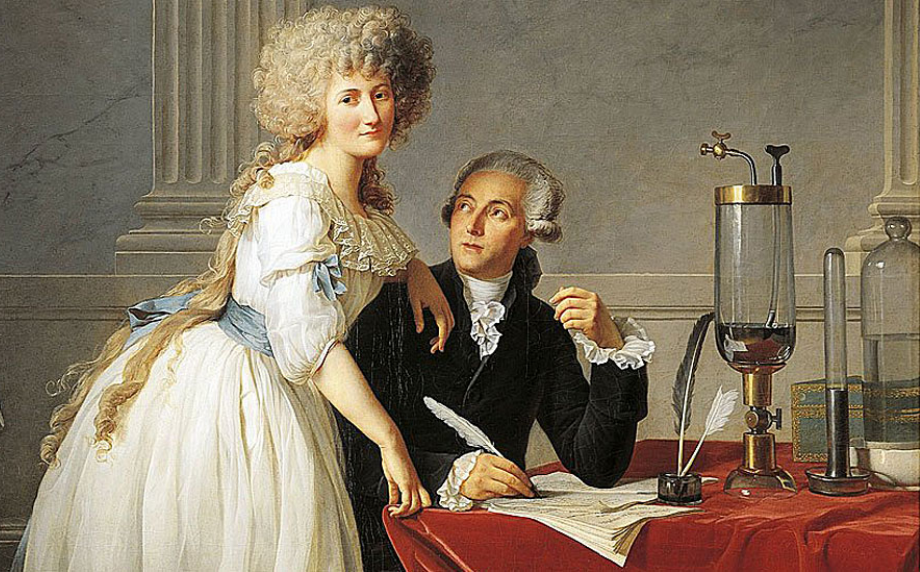
\includegraphics[width=1\linewidth]{imagens/figura 4.png} 
	\caption{Antoine-Laurent de Lavoisier e Marie-Anne Pierretti Paulze}
	\label{fig:wrapfig}
\end{figure}

Muitos pesquisadores e entusiastas realizavam (sem muito planejamento) todo tipo de experimentação, o que criou, por exemplo, o ofício de perfumista. A curiosidade os levava a analisar diversos materiais e organismos em busca de sua composição e, por causa de empreitadas assim, muitas substâncias forma descobertas, inclusive com aplicações médicas, mas tudo a partir daqui esbarrava em uma barreira até então intransponível: não era possível produzir artificialmente uma substância de origem vegetal ou animal, e apenas tais organismos possuíam uma misteriosa "força vital" \index{Força vital} que os permitia produzir tais substâncias. Concorda que fica mais fácil atribuir dificuldades a forças misteriosas e/ou sobrenaturais?

Neste momento da história, definia-se Química Orgânica como "a parte da Química que estuda substâncias obtidas de organismos vivos", os portadores da Força Vital. Mas o tempo passou novamente e chegamos em 1828, na Alemanha.

\chapter{Salve, Wöhler!}
A Química possui muitos nomes de destaque ao longo da história, como o próprio Lavoisier, Berzelius, Van't Hoff, Grignard, entre muitos outros. O próximo nome de destaque saiu de sua terra natal para estudar com Berzelius em pessoa, em Estocolomo. A Universidade de Göttingen, onde Friedrich Wöhler \index{Wöhler} tornou-se docente, tornou-se um celeiro de grandes nomes para a ciência, como Gauss, Fermi, Pauli, entre muitos outros.

Wöhler era muito dedicado à ciência de modo geral, uma vez que sua atuação como químico não era a única de sua carreira, pois atuou também como obstetra, mas uma de suas atividades ajudou a mudar os rumos da Química Orgânica, até o momento restrita a substâncias extraídas de seres vivo, daí a origem do chamado Vitalismo, com já discutido anteriormente.

Embora tenha sido considerado o estopim da derrocada do Vitalismo, este perdurou ainda por anos devido, em parte, à dificuldade em aceitar algo radicalmente diferente e, podemos dizer, até certo ponto iconoclasta. O declínio do vitalismo começou a ficar mais evidente em 1843, quando Hermann Kopp defendeu que a Síntese de Wöhler (uma delas) foi o ponto de partida para o abandono de teorias vitalistas. Mas qual seria essa tão marcante reação?

Na realidade, não foi apenas uma reação pontual, mas algumas que, combinadas em sequência, levaram à produção de ureia \index{Ureia}. Uma representativa desse processo pode ser vista na figura a seguir.

\begin{figure}[h]
	\centering
	\caption{Uma das etapas da síntese da ureia}
	\vspace{0.5cm}
	\label{fig:captura-de-tela-de-2023-07-15-20-28-19}
	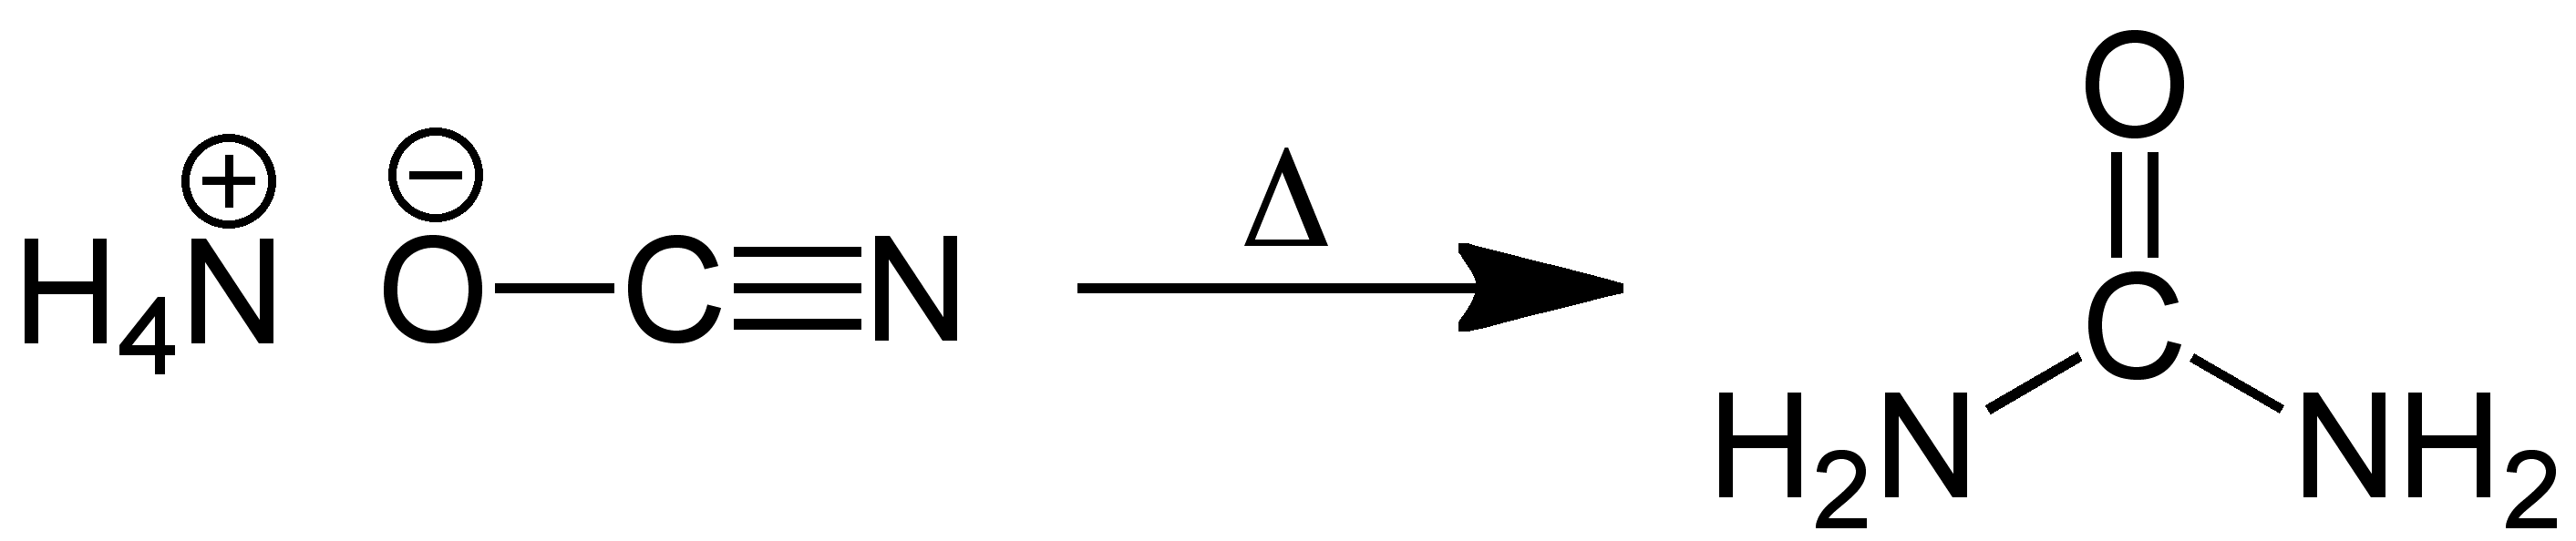
\includegraphics[width=0.7\linewidth]{imagens/Urea_Synthesis_Woehler.png}
\end{figure}

Esqueça, por um momento, que Wöhler era aluno de Berzelius, um dos mais fervorosos defensores do vitalismo, este mortalmente ferido com a síntese de Wöhler. Qual foi uma consequência real de todo esse processo? A síntese de muitas outras substâncias orgânicas, como medicamentos, fertilizantes, entre muitos outros tipos. Por razões estritamente pessoais, o autor deste livro exemplifica a molécula do taxol \index{Taxol} como uma consequência do feito de Wöhler, como pode ser visto na \ref{fig:taxol}

\begin{figure}[h]
	\centering
	\caption{Estrutura do taxol, uma substância polifuncional contendo as funções álcool, cetona, éter, amida e éster.}
	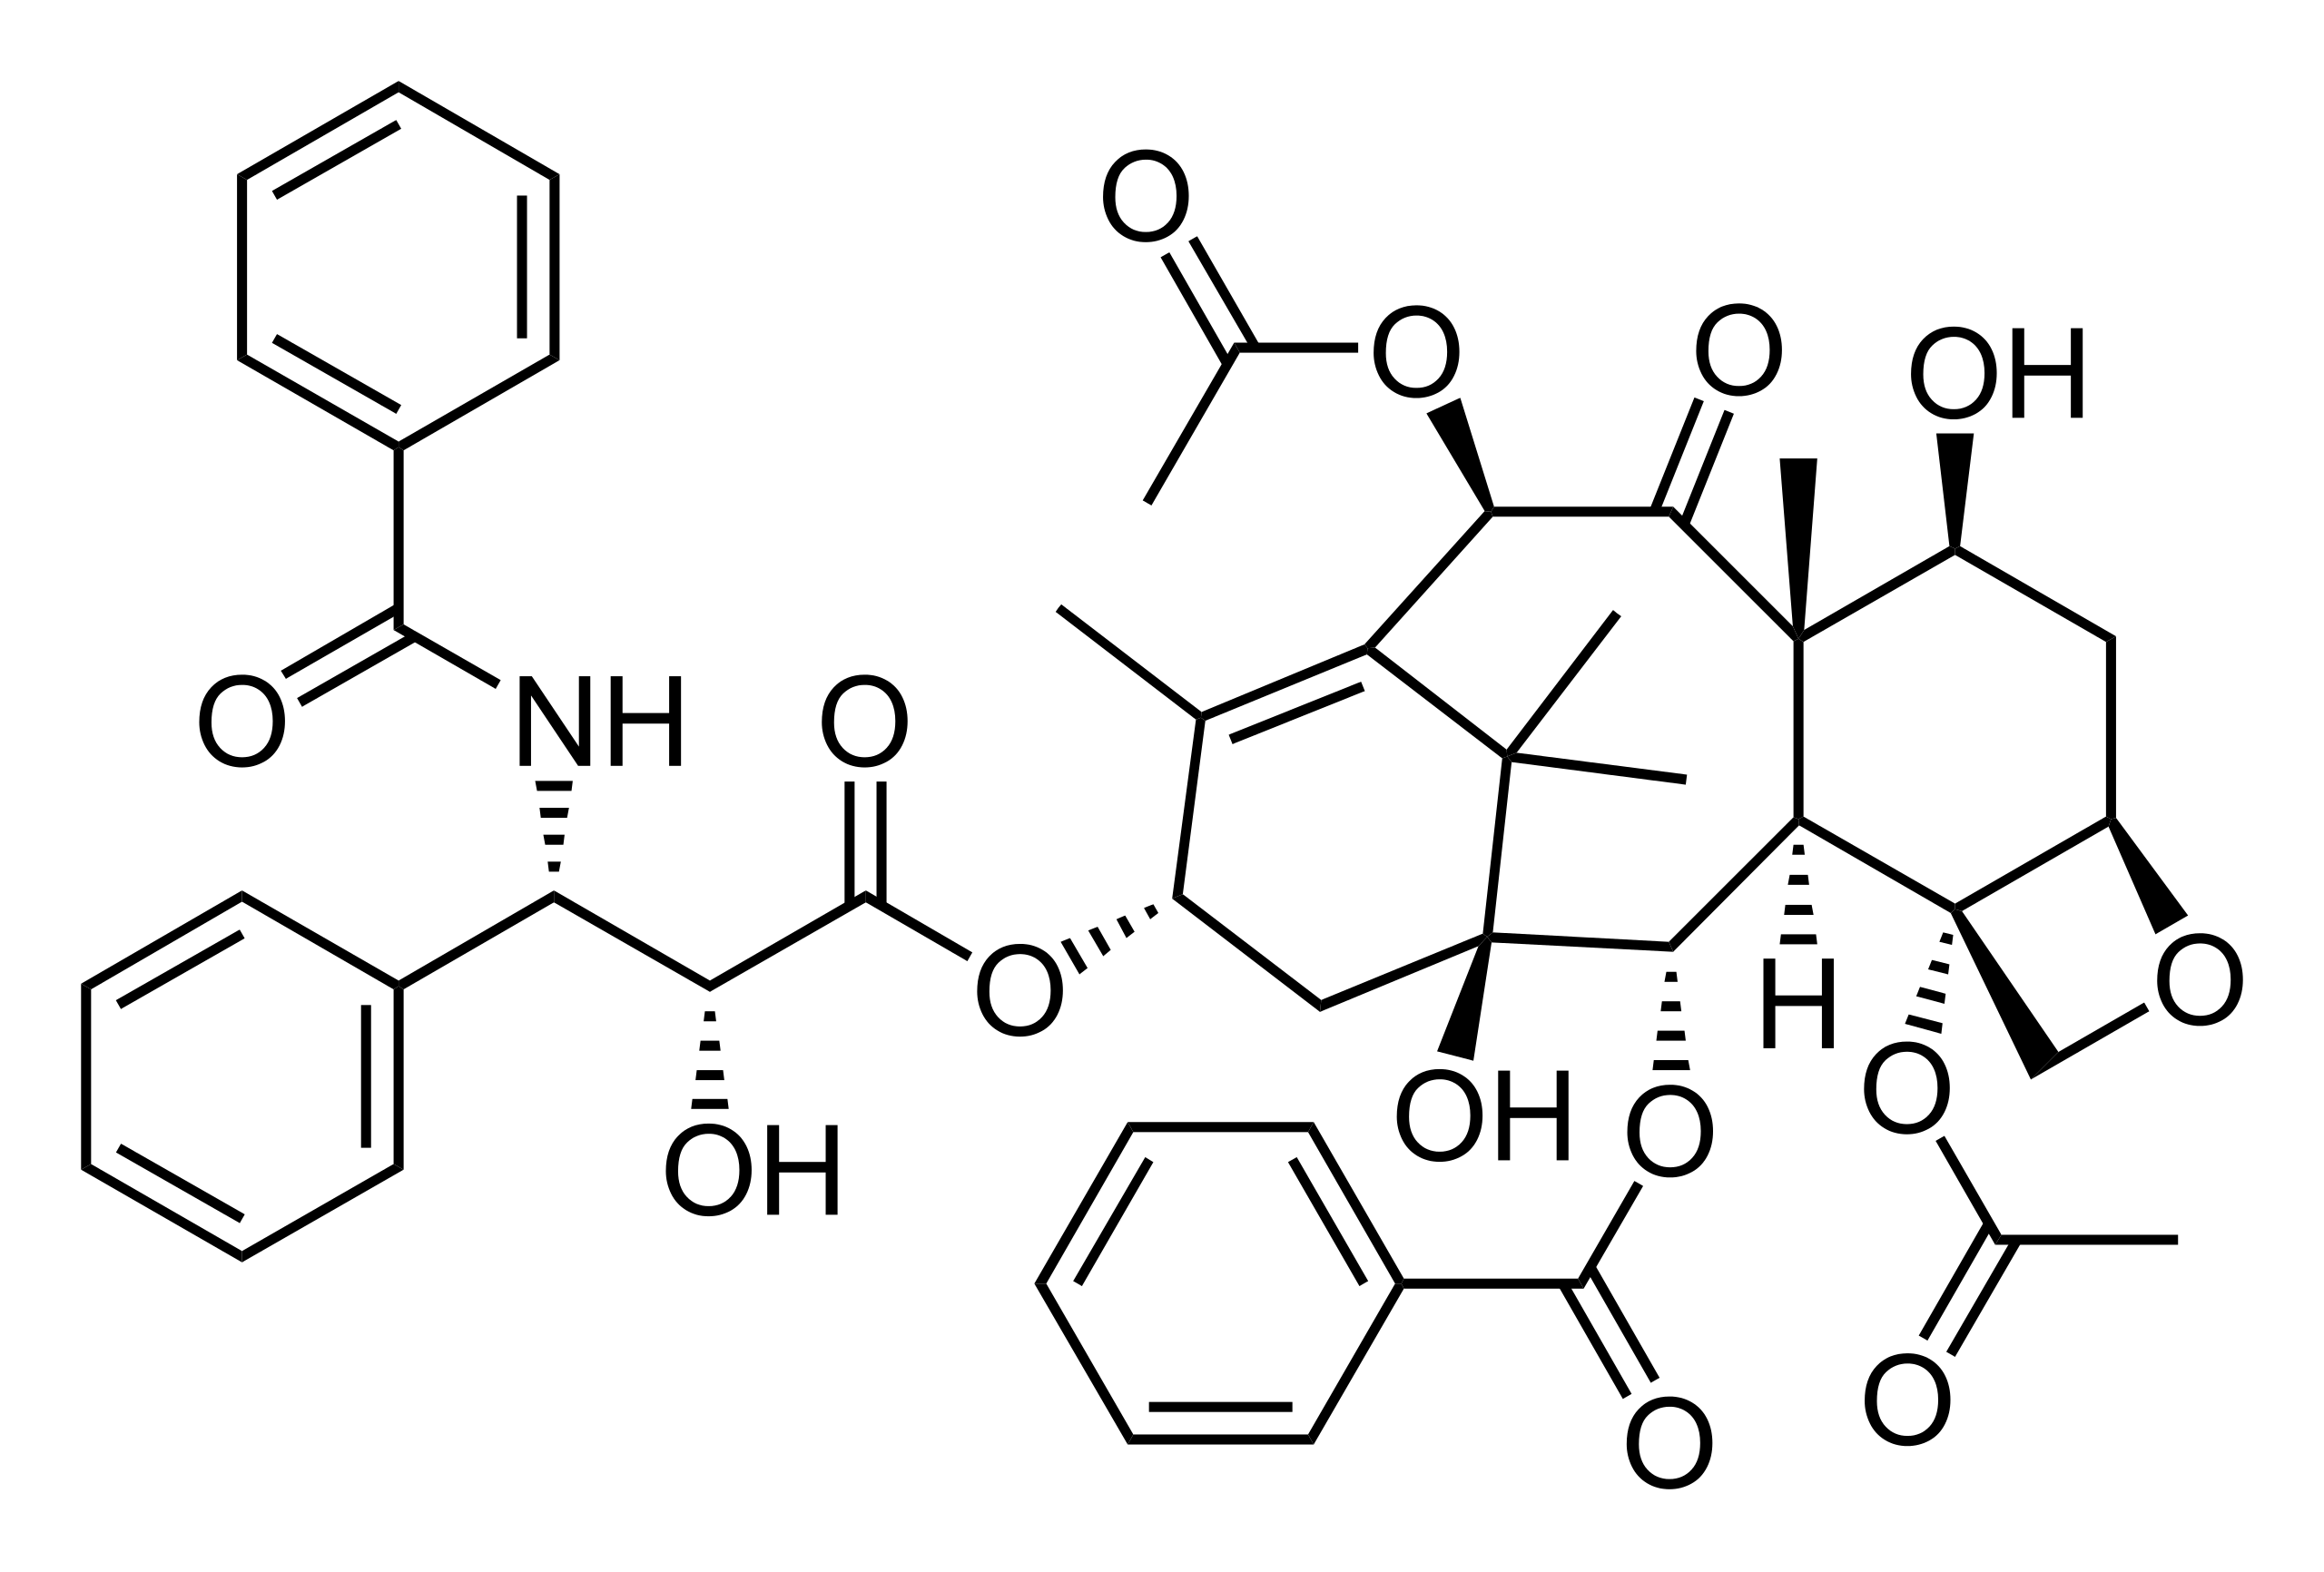
\includegraphics[width=0.3\linewidth]{imagens/Taxol.svg.png} 
	\label{fig:taxol}
	\caption*{Fonte: Autores}
\end{figure}


O que move a ciência é o questionamento: como alguém descobriu que essa molécula é encontrada nessa árvore em especial? A resposta e simples e cristalina como água pura.

Na década de 1960, o National Cancer Institute (NCI), nos EUA, iniciou um programa ambicioso de screening, ou seja, busca, por substância naturais com potencial atividade antitumoral e foram coletadas mais de 35000 amostras de plantas diferentes, no país todo. Perto de 10 anos após a coleta, uma substância chamada paclitaxel, com potencial ação antitumoral, foi encontrada e tornou-se medicamento aprovado em 1992, quase 30 anos após o início do projeto de screening.

A ação do taxol está relacionada com a estabilização dos microtúbulos, impedindo que ocorra a despolimerização e causando a morte celular, uma vez que os microtúbulos são intimamente relacionados com a estabilidade da parede celular de células eucarióticas. Sua síntese foi muito aguardada e disputada no meio químico, pois foi necessário abater 38000 árvores para obter a quantidade de moléculas necessárias para tratar os 12000 paciente dos ensaios clínicos in vivo.

Esteja onde estiver, Wöhler, esta conquista é sua!

\part{O todo-poderoso carbono}

\chapter{Ligação química carbono-carbono}
Falar sobre as diferentes ligações covalentes que dois átomos de carbono podem realizar requer o embasamento teórico proveniente do Modelo Atômico atual e também das Combinações Lineares de Orbitais Atômicos \index{CLOA}, o que explica as ligações conhecidas como sigma, pi e também explica a deslocalização eletrônica em sistemas insaturados.

A necessidade de criação de um novo modelo organizacional para a eletrosfera do átomo trouxe consigo a criação de novas entidades conhecidas como orbitais atômicos, ou seja, uma região da eletrosfera onde é máxima a probabilidade de encontrarmos um dado elétrons. Pensando de maneira simples e sem mergulhar na complexa matemática envolvida, cada um dos elétrons de um átomo possui algo semelhante a um endereço eletrônico, conhecido como números quânticos. Cada um destes é capaz de apontar, dentro das limitações conceituais do modelo e visualização de um elétron, onde cada elétron pode ficar na eletrosfera de qualquer átomo.

A distribuição dos elétrons pela eletrosfera de cada átomo determina suas propriedades químicas e espectroscópicas, por exemplo, o que ajuda a caracterizar as ligações químicas que ocorrem entre dois átomos de carbono. Para compreender plenamente estrutura e reatividade de compostos orgânicos, precisamos analisar como se formam as ligações químicas que o carbono realiza, no total de quatro, conforme já descrido há décadas por Friedrich August Kekule, no longínquo ano de 1857.

O Modelo Atômico Atual (MAA) permite a organização da eletrosfera em níveis de energia (equivalentes ao conceito de camadas eletrônicas, propostas por Bohr), subníveis de energia (conceito novo em relação a Bohr), compreendidos como conjunto de orbitais, este último algo bastante abstrato, mas de fundamental importância daqui em diante, pois o comportamento químico de algumas ligações e funções depende dese conceito.

\section{Orbitais e suas formas}
Pense em um orbital como um local no espaço, matematicamente definido, onde é máxima a probabilidade de encontrarmos um elétron. Sabendo que os orbitais possuem formas distintas, pois são soluções de parte das equações que definem o MAA. Repare no refinamento conceitual se comparado com as ”órbitas”de Rutherford ou então com as ”camadas”de Bohr. A figura \ref{fig:orbitais} a seguir apresenta as formas dos diferentes orbitais utilizados até o momento.

\begin{figure}[h]
	\caption{Orbitais atômicos}
	\vspace{0.25cm}
	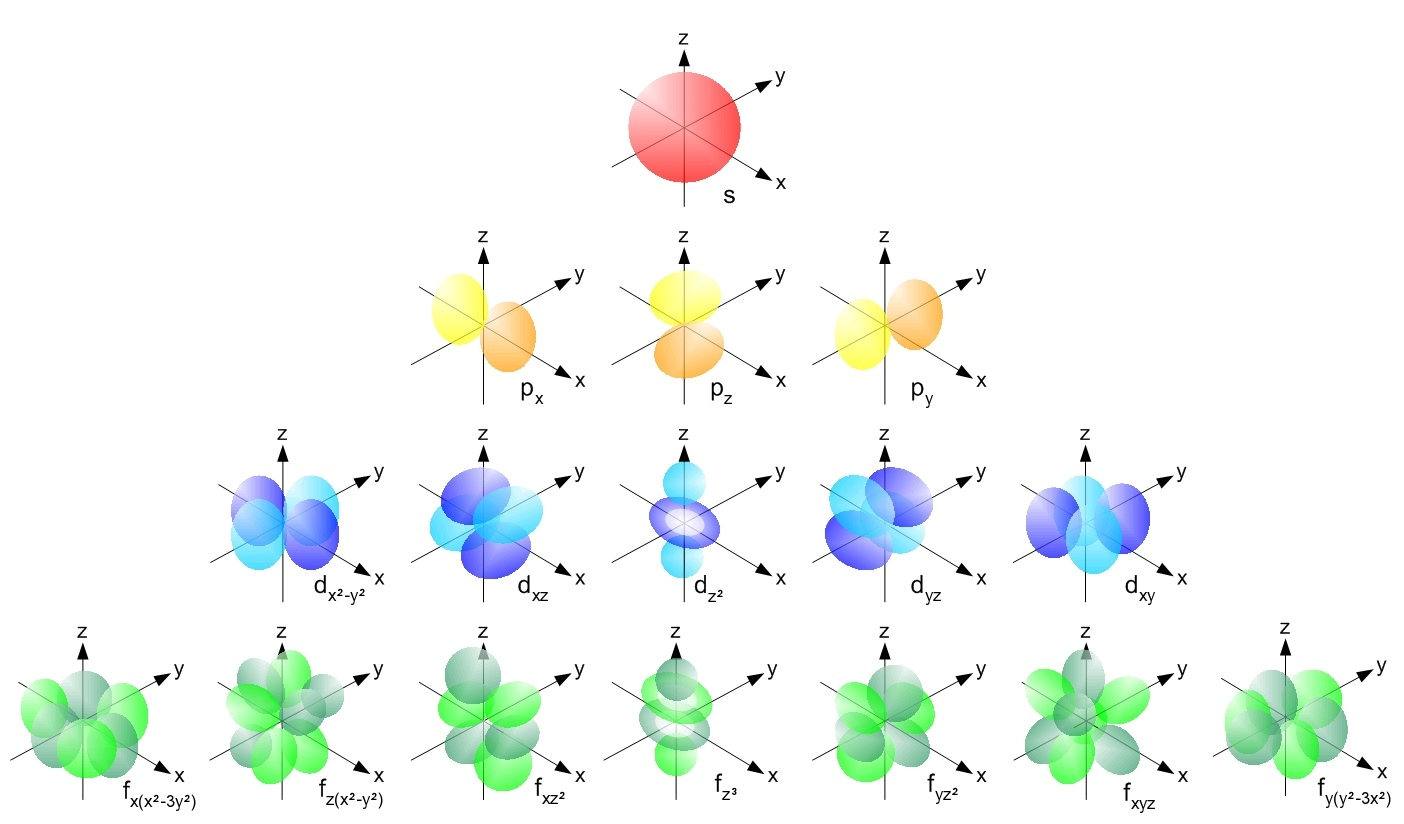
\includegraphics[width=1\linewidth]{imagens/figura8_orbitais.jpg} 
	\label{fig:orbitais}
\end{figure}

Cada parte colorida da figura acima indica os locais onde elétrons podem ser encontrados. O subnível s, que aparece na primeira linha da figura, é formado por apenas um orbital de forma esférica e os dois elétrons que esse orbital pode acomodar (assim como todos os demais orbitais) podem ocupar qualquer posição dentro da esfera.

A segunda linha da figura apresenta o chamado subnível p, composto por três orbitais orientados em um sistema tridimensional e cada orbital é indicado de acordo com o eixo de orientação no qual se encontra: px, py e pz. Vale o mesmo raciocínio para os demais orbitais, mas nosso foco será no carbono.

Nos diferentes eixos de orientação é possível encontrar regiões nas quais a probabilidade de encontrar um elétron é zero, o que é matematicamente consistente com a modelagem matemática envolvida. A figura \ref{fig:orbitaisp} a seguir ilustra o chamado plano nodal presente nos orbitais do tipo p.

Porém, quando unimos este modelo com a distribuição eletrônica no estado fundamental para o carbono, percebemos uma aparente inconsistência: 1s22s22p2. De acordo com essa distribuição eletrônica, e lembrando da Regra da Máxima Multiplicidade de Hund e que cada orbital acomoda até dois elétrons, de acordo com o Princípio da Exclusão de Pauli, o átomo de carbono só formaria 2 ligações covalentes, contradizendo o conhecimento secular trazido por Kekule. 

\begin{figure}[h]
	\centering
	\caption{Planos nodais nos orbitais p}
	\vspace{0.25cm}
	\label{fig:orbitaisp}
	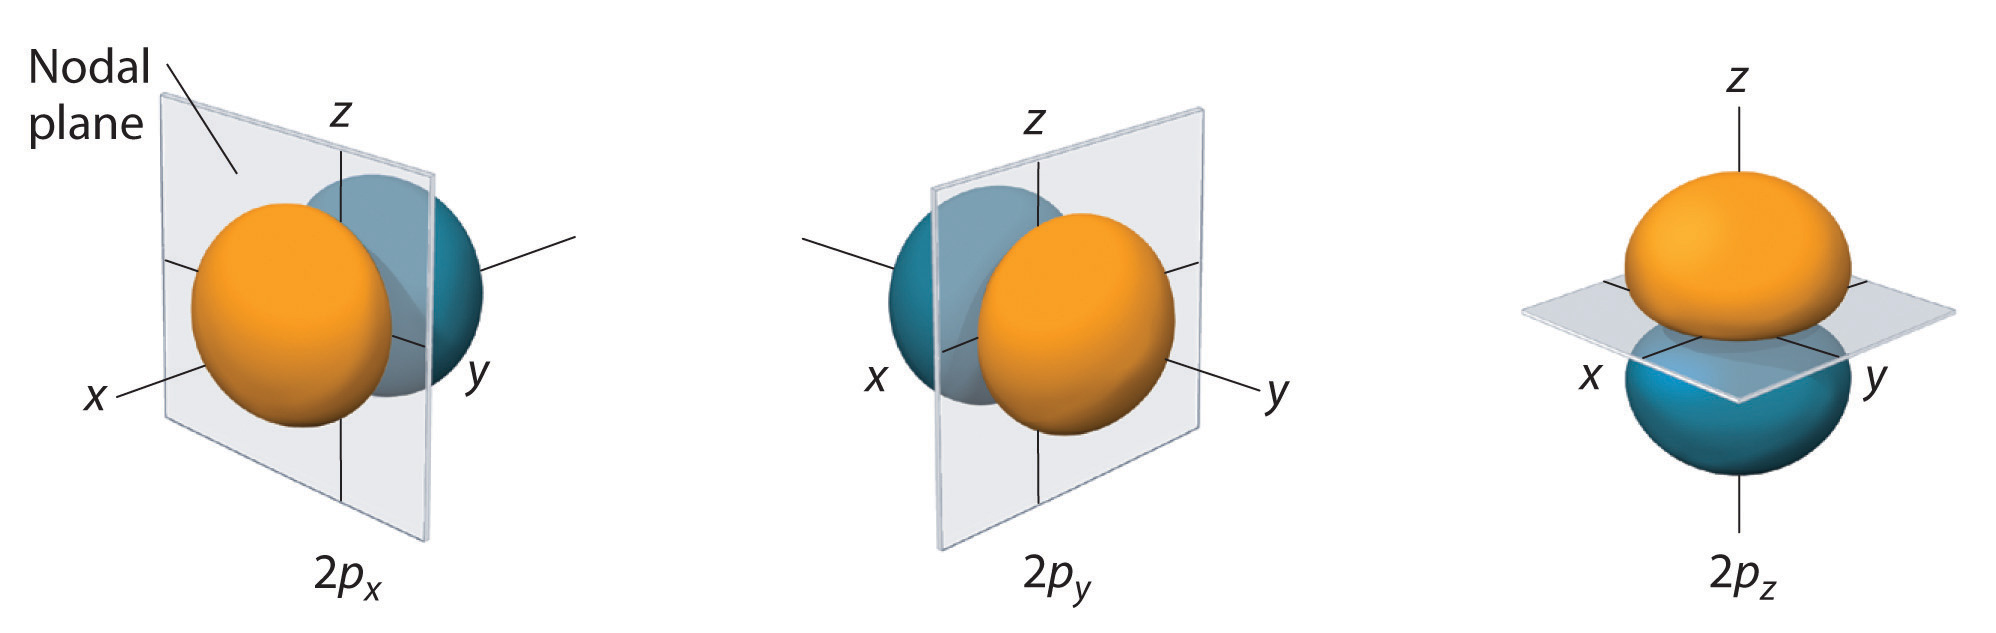
\includegraphics[width=\linewidth]{imagens/plano_nodal.jpeg}
\end{figure}

A figura \ref{fig:hibridacao}, apresentada a seguir, a parte superior indicada por ground state (ou estado fundamental) mostra como é a configuração eletrônica para o átomo de carbono. Embora pareça bem estranho, a promoção de um elétron de um um subnível a outro deixa os subníveis envolvidos em um estado energético chamado de "degenerado", ou seja, em igualdade energética.

Para níveis energéticos baixos, especialmente o nível 2, os valores de energia dos subníveis s e p são muito próximos, obedecendo aos princípios de Bohr, o que justifica a facilidade com que ocorre o fenômeno da hibridização, lembrando que tal situação se verifica apenas no momento da ligação química e precisa ficar claro que átomos isolados não possuem orbitais híbridos.

Átomos multieletrônicos apresentam o chamado efeito de blindagem e, portanto, os elétrons de camadas mais externas sofrem diferentes atrações por parte do núcleo positivo, e isso ajuda a entender a diferença de energia verificada entre subníveis.

\begin{figure}[h]
	\centering
	\caption{Hibridização no carbono}
	\vspace{0.25cm}
	\label{fig:hibridacao}
	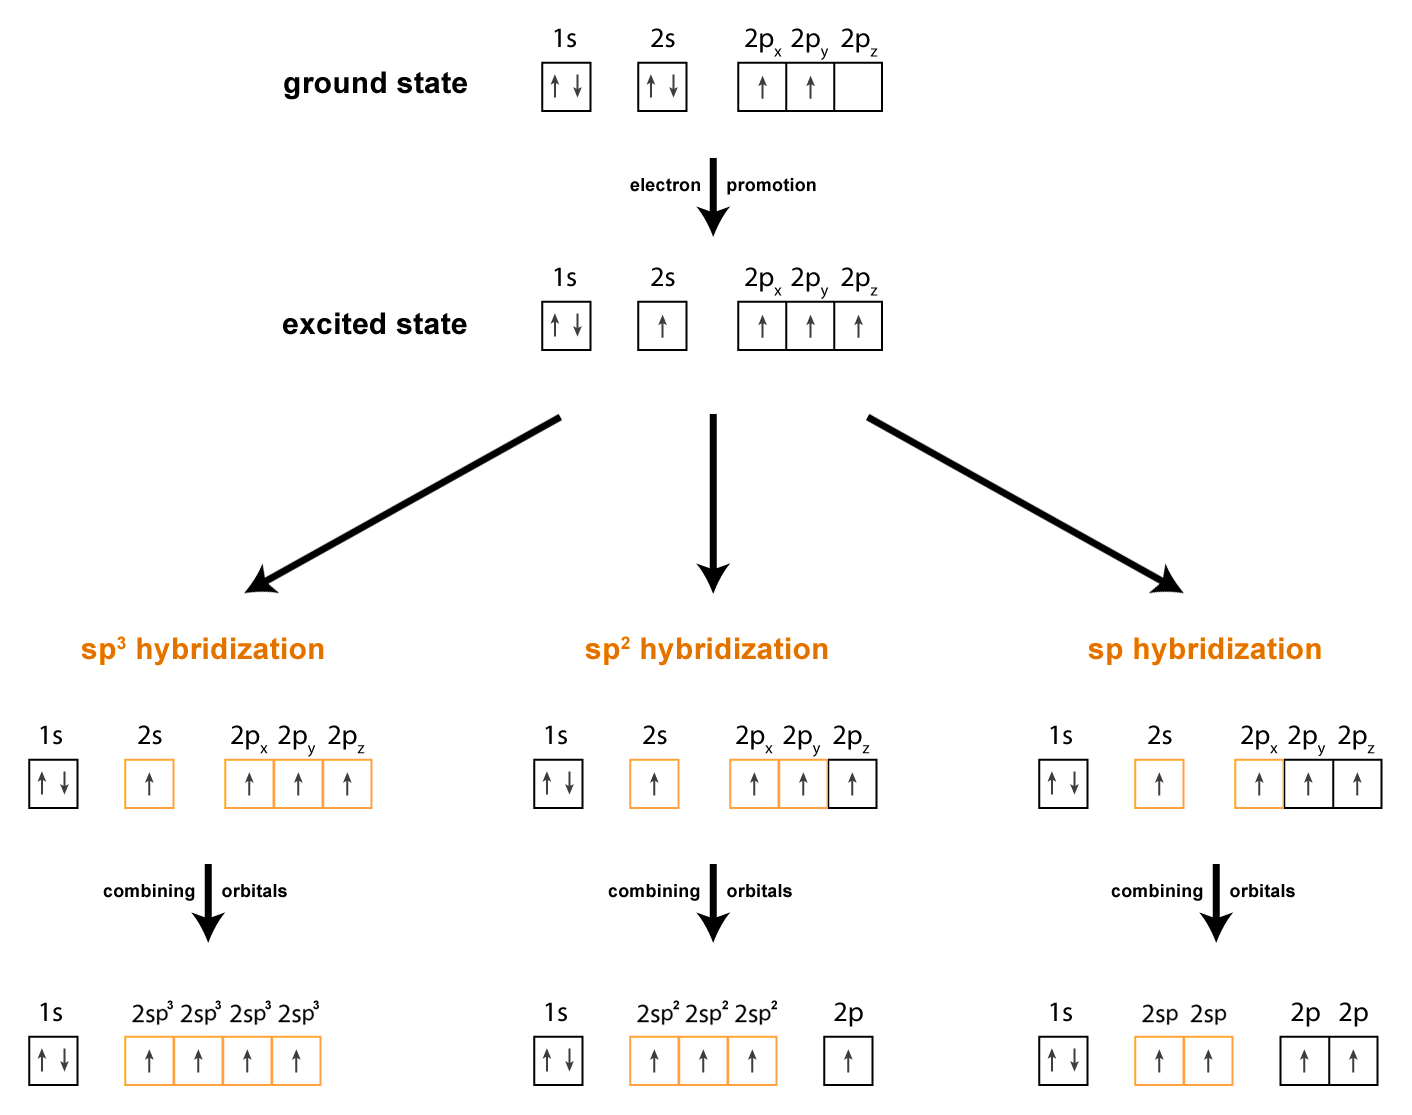
\includegraphics[width=1\linewidth]{imagens/figura9_hibridacao.png}
\end{figure}

Uma vez que a ligação covalente é formada pelo compartilhamento de dois elétrons originados de átomos diferentes, não há como o carbono ser tetravalente, a não ser que a configuração eletrônica se altere, e tal alteração se dá pela combinação matemática de um orbital 2s com todo o subnível 2p. Tal combinação chama-se hibridização.

A hibridização é um conceito da química que descreve a mistura de orbitais atômicos para formar novos orbitais híbridos. Os orbitais híbridos têm formas e energias diferentes dos orbitais atômicos originais.

O carbono é um elemento que pode se hibridizar de várias maneiras. A hibridização mais comum do carbono é sp3, que ocorre quando o carbono forma quatro ligações covalentes e podemos dizer, também que este carbono é dito  \textbf{saturado}. Na hibridização sp3, o carbono combina um orbital s e três orbitais p para formar quatro novos orbitais híbridos sp3. Esses orbitais híbridos são orientados a 109,5 graus uns dos outros e formam ângulos de ligação de 109,5 graus, caracterizando a chamada "geometria tetraédrica".

Uma vez que justificamos a tetravalência do carbono, podemos explorar agora dois conceitos bastante comuns daqui em diante: ligação sigma ($\sigma$) e ligação pi ($\pi$). São dois tipos de ligações semelhantes porque ocorrem da mesma forma: sobreposição de orbitais, sejam puros ou híbridos, mas ao mesmo tempo diferentes porque a orientação da sobreposição é diferente: observamos \textbf{sobreposição frontal} de orbitais na ligação sigma ($\sigma$) e \textbf{sobreposição lateral} de orbitais na ligação pi ($\pi$). Parece pouca diferença, mas está longe disso, pois características como distância e entalpia de lição são bem diferentes dois casos, sem citar a reatividade relativa entre os dois tipos de ligação, entre várias outras características de diferenciação. Veja uma justificativa parcial na figura \ref*{fig:sdt}:

\begin{figure}[h]
	\centering
	\caption{Comprimento de ligação e entalpias de ligação C-C}
	\vspace{0.25cm}
	\label{fig:sdt}
	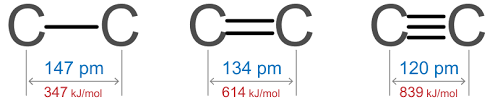
\includegraphics[width=0.85\linewidth]{imagens/sdt.png}
\end{figure}

Cabe uma pergunta aqui, imediatamente: por que existem esses três tipos de ligações C-C? Toda boa pergunta merece uma boa resposta e começa pela análise da figura \ref*{fig:sigma} a seguir.

\begin{figure}[h]
	\centering
	\caption{Sobreposição frontal de orbitais}
	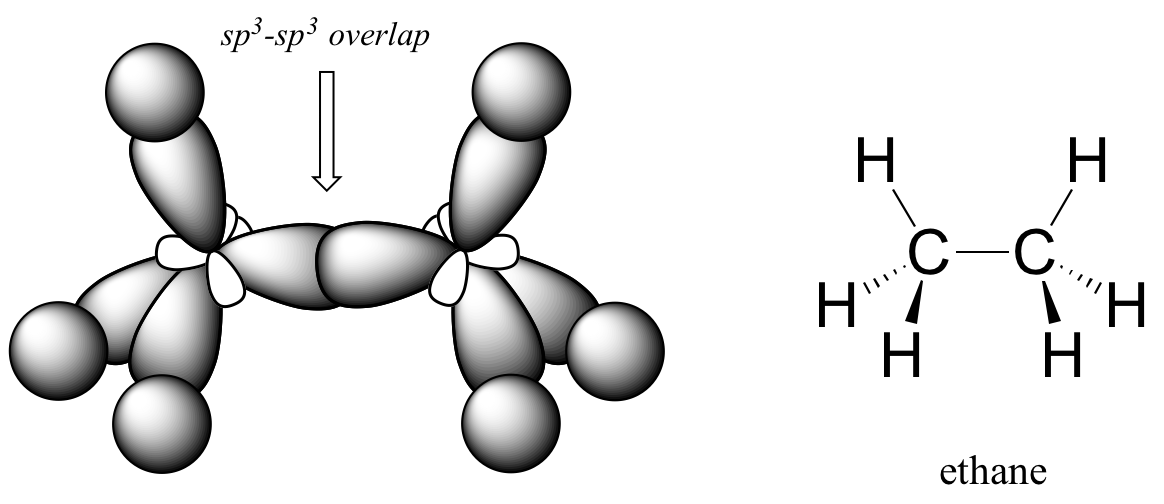
\includegraphics[width=0.5\linewidth]{imagens/sp3overlap.jpg}
	\label{fig:sigma}
\end{figure}

O leitor que já passou pelo chamado Ensino Médio certamente se lembra (ou deveria lembrar-se) da representação de ligações covalentes, por um traço simples. Aquela é a representação simplificada da ligação sigma.

\begin{figure}[h]
	\centering
	\caption{Representação esquemática do metano}
	\label{fig:metano}
	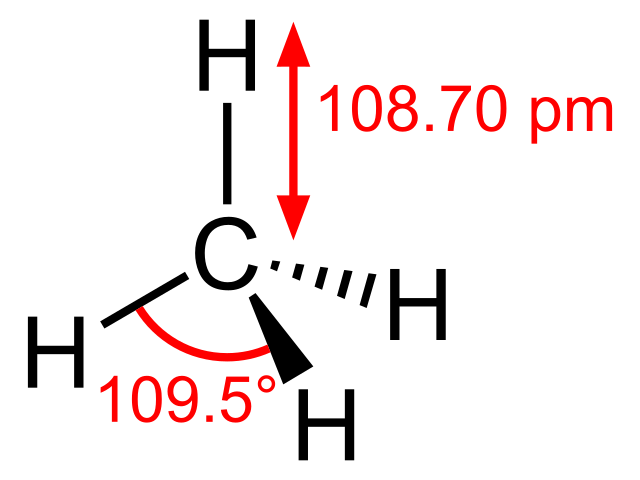
\includegraphics[width=0.4\linewidth]{imagens/Methane-2D-dimensions.svg.png}
\end{figure}

Ganhando tempo para quando analisarmos os conceitos muito importantes de Estereoquímica, a imagem \ref{fig:metano} apresenta, aparentemente, três tipos de ligações químicas. A expressão "aparentemente" se justifica porque tentamos representar uma molécula tridimensional em um espaço bidimensional (a página deste livro). A ligação representada por um traço indica uma ligação presente no chamado plano de referência, algo como uma mesa ou placa de vidro. A ligação tracejada indica que a ligação está orientada especialmente para trás do plano de referência e, finalmente, a ligação que lembra um pequeno triângulo indica que a ligação está orientada para a frente do plano de referência. É uma saída para representar três dimensões em apernas duas disponíveis. Faça um exercício, caro leitor: analise novamente a molécula do taxol, representada na figura \ref{fig:captura-de-tela-de-2023-07-15-20-28-19}, e a imagine em três dimensões.

Chegou o momento de analisarmos a chamada sobreposição lateral de orbitais, a responsável pela ligação pi. Esse tipo de sobreposição só ocorre nas hibridizações \textbf{sp{$^2$}} ou \textbf{sp}, nas quais restam um ou dois orbitais p puros que não participaram da combinação linear de orbitais atômicos.

O leitor atento já deve ter percebido, analisando a figura \ref{fig:ligacaopi}, que uma eventual sobreposição de orbitais que não seja frontal tende a ser menos eficiente, por razões de proximidade espacial dos orbitais p puros. A figura \ref{fig:ligacaopi} a seguir ajuda a esclarecer o assunto.

\begin{figure}[h]
	\centering
	\caption{Ligação pi}
	\vspace{0.5cm}
	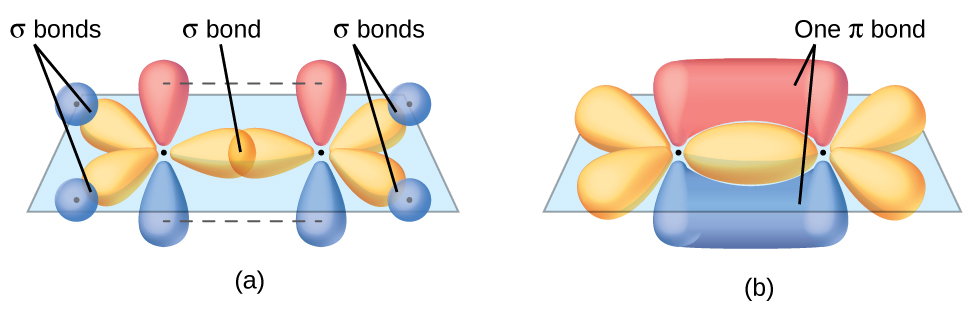
\includegraphics[width=0.85\linewidth]{imagens/doublebond.jpeg}
	\label{fig:ligacaopi}
\end{figure}

Embora o orbital p tenha esse formado de halteres, considere que os elétrons ocupem a porção superior ou então a porção inferior do orbital. Assim, a ligação pi é formada pelo compartilhamento de quatro elétrons entre dois átomos: dois formando a ligação sigma e outros dois formando a ligação pi. Mas fique atento, leitor: como o orbital puro possui dois nós, a ligação pi possui duas partes, uma cima a outra abaixo da ligação sigma. Isso explica muitas características de carbonos insaturados, aqueles átomos que formam ligações duplas.

Devemos salientar que a hibridização sp{$^2$} gera um conjunto de três orbitais híbridos com arranjo planar e separados entre si or um ângulo de 120 graus, o que caracteriza a chamada "geometria trigonal plana". Esta geometria virá à tona novamente quando analisarmos reações químicas envolvendo um grupo funcional chamado carbonila, como será visto em outro ponto deste livro.

Existe mais uma possibilidade de hibridização para o carbono, aquela que envolve um orbital 2s e apenas um dos orbitais 2p, formando um conjunto de dois orbitais híbridos sp e deixando dois orbitais p puros. Seguindo o mesmo raciocínio da formação da ligação carbono-carbono dupla, quando dois átomos de carbono com hibridização sp de aproximam, forma-se uma ligação sigma sp-sp e duas ligações pi, totalizando três pares de elétrons entre os dois átomos e a ligação é representada por três traços, conforme pode ser visto na figura \ref{fig:ligacaotripla2}

\begin{figure}[h]
	\centering
	\caption{Ligação tripla}
	\vspace{0.5cm}
	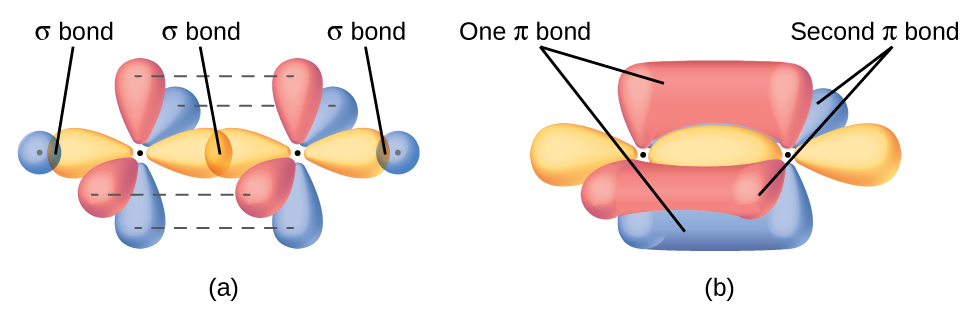
\includegraphics[width=0.85\linewidth]{imagens/triplebond.jpeg}
	\label{fig:ligacaotripla2}
\end{figure}

A simples análise da figura \ref*{fig:ligacaotripla2} mostra que o orbital molecular formado pela sobreposição frontal dos orbitais híbridos sp deixa os átomos de carbono com mais uma ligação sigma a realizar e esta orienta-se no espaço de forma diametralmente oposta ao orbital molecular. Assim, o átomo de carbono com hibridização sp assume a chamada "geometria linear".

\section{Sobre geometria molecular}
A hibridização dos átomos de carbono é importante porque determina a forma das moléculas e os ângulos de ligação entre os átomos. A forma das moléculas e os ângulos de ligação podem afetar as propriedades físicas e químicas das moléculas. O que define esses ângulos?

A teoria de repulsão dos pares de elétrons da camada de valência (VSEPR - Valence Shell Electronic Pair Repulsion) é uma teoria química que descreve a geometria molecular das moléculas. A teoria VSEPR afirma que a geometria molecular de uma molécula é determinada pela forma como os pares de elétrons da camada de valência (pares de elétrons ligantes e pares de elétrons não ligantes) se repelem uns aos outros.

A teoria VSEPR pode ser usada para prever a geometria molecular de uma grande variedade de moléculas. Por exemplo, a molécula de água tem uma geometria angular porque o átomo de oxigênio tem dois pares de elétrons ligantes e dois pares de elétrons não ligantes. Os pares de elétrons ligantes e não ligantes se repelem uns aos outros, o que resulta em uma geometria angular.

\begin{figure}[h]
	\centering
	\caption{Geometria da molécula de água}
	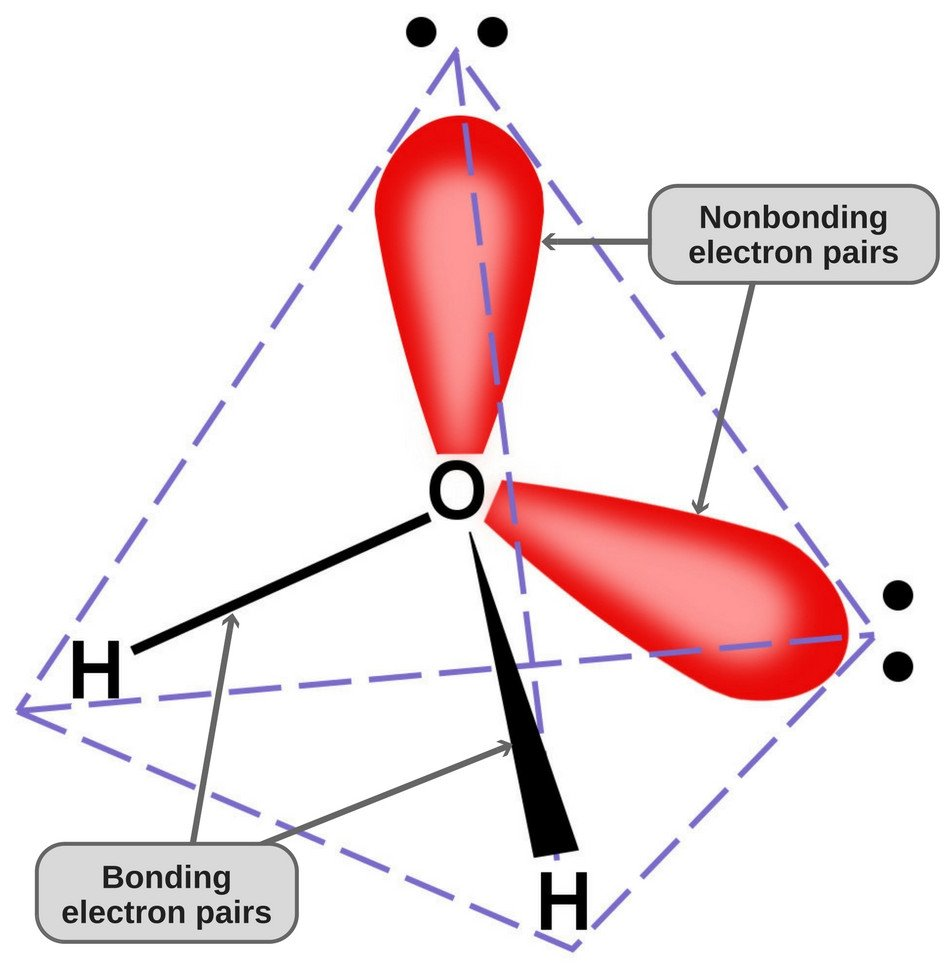
\includegraphics[width=0.45\linewidth]{imagens/is_water_a_tetrahedral_molecule.jpg}
	\label{fig:vsepragua}
\end{figure}

A teoria \label{vsepr}VSEPR também pode ser usada para prever o ângulo de ligação entre os átomos de uma molécula. O ângulo de ligação é o ângulo entre os pares de elétrons ligantes de uma molécula. Por exemplo, o ângulo de ligação na molécula de água é de 104,5 graus. Esse ângulo é determinado pela forma como os pares de elétrons ligantes e não ligantes se repelem uns aos outros.

A teoria VSEPR é uma ferramenta útil para prever a geometria molecular e o ângulo de ligação das moléculas. No entanto, é importante observar que a teoria VSEPR não é perfeita. Existem algumas moléculas que não seguem as previsões da teoria VSEPR. Isso ocorre porque a teoria VSEPR não leva em consideração fatores como a repulsão entre os núcleos atômicos e a interação de elétrons de valência com elétrons de camadas internas.

\section{O conceito de ressonância e suas aplicações}
Se você chegou até este ponto do texto, certamente se lembra de ter visto, em algum momento de dua vida acadêmica, a expressão "Estrutura de Lewis" ou algo bem semelhante. Tudo funciona muito bem até o ponto onde uma única estrutura de Lewis não é capaz de descrever uma molécula. Quando isso ocorre, múltiplas estruturas de Lewis podem ser usadas para descrever uma molécula e isso recebe o nome de \textbf{ressonância. }Mas como isso é possível?

Antes de falarmos a respeito de outras moléculas orgânicas mais complexas, precisamos entender claramente o conceito de ressonância, o que ajuda a explicar parte do conceito de acidez/basicidade. Para tanto, usaremos o gás ozônio, de fórmula O{$_3$}, para ilustrar o conceito de ressonância.

Durante o processo de montagem da estrutura de Lewis para o ozônio, você deve chegar à etapa representada pela figura a seguir, onde faltam colocar dois elétrons no átomo central e resta a pergunta mais crítica: você usará dois elétrons do átomo de oxigênio da esquerda ou do átomo da direita?

\begin{figure}[h]
	\centering
	\caption{Estrutura de Lewis parcialmente completa para o ozônio}
	\vspace{0.5cm}
	\label{fig:lewis}
	
\includegraphics[width=1\linewidth]{imagens/o3parcial.jpg}
\end{figure}

Analise friamente: não há diferença em usar um dos pares eletrônicos citados, pois chegaremos ao mesmo resultado, mas ao mesmo tempo não podemos simplesmente deixar o acaso escolher algo assim tão sério. Por tal motivo, consideramos corretas o uso de qualquer um dos dois pares eletrônicos e fica mais adequado representar as duas estruturas de Lewis possíveis para o ozônio, conforme pode ser visto na figura \ref*{fig:ozonio}. Então, é conceitualmente mais adequado dizer que a estrutura de Lewis correta para o ozônio é a média das duas estruturas possíveis, o que explica a dupla seta presente na figura.

\begin{figure}[h]
	\centering
	\caption{Estruturas de ressonância para o ozônio}
	\vspace{0.5cm}
	\label{fig:ozonio}
	
\includegraphics[width=1\linewidth]{imagens/o3completo.jpeg}
\end{figure}

Para finalizar a conversa sobre ressonância, analise as estruturas de ressonância possíveis para o ânion sulfato, SO{$_4$}{$^{2-}$}, e entenda a razão pela qual nem toda molécula que possui um hidrogênio ligado a átomo muito eletronegativo pode ser considerada um ácido de Arrhenius. Entende agora porque o etanol, CH{$_3$}CH{$_2$}OH, não apresenta caráter ácido? Não existe uma estrutura de ressonância capaz de estabilizar a carga negativa existente após a saída do cátion hidrônio.

\begin{figure}[h]
	\centering
	\caption{Estruturas de ressonância para o ânion sulfato}
	\label{fig:sulfato}
	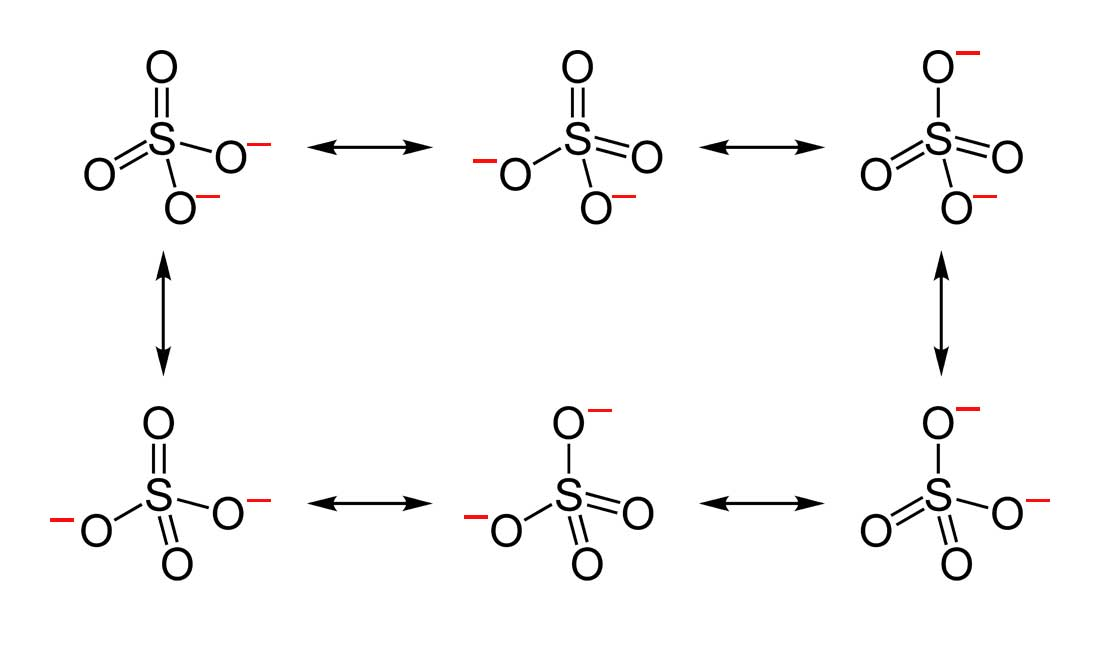
\includegraphics[width=0.5\linewidth]{imagens/Sulfate-resonance.jpg}
\end{figure}

Ok, mas como isso aparece em moléculas orgânicas mais complexas?

\section{Aromaticidade}
Falamos sobre um dos pontos principais da aromaticidade há poucos parágrafos: orbitais moleculares. Apenas para lembrar quem passou rapidamente por aquele tema, um \textbf{orbital molecular} (OM) forma-se pela combinação de orbitais atômicos, sejam puros ou híbridos. Esses OM podem ser do tipo \textbf{ligante} ou \textbf{anti-ligante}, para simplificar o assunto.

De forma geral, observa-se que orbitais moleculares \textbf{ligantes} preenchidos com dois elétrons {$\pi$} levam a molécula a uma situação de bastante baixo conteúdo de energia, conhecido por \textbf{estabilidade}. 

A análise simples da estrutura presente na \ref{fig:nenzenodetalhes} mostra a molécula do benzeno com 3 ligações duplas, ou seja 6 elétrons {$\pi$}. Além disso, todos os átomos de carbono de sua estrutura apresentam geometria \textbf{trigonal plana} e, portanto, apresentam hibridização sp{$^2$}. Isso faz com que os orbitais p que formam a ligação dupla estejam próximos o suficiente para permitir a ressonância, fazendo com que o benzeno apresente três estruturas de ressonância rapidamente intercambiáveis. Assim, não é muito adequado usar nenhuma delas individualmente, mas sim todas ao mesmo tempo. Um sumário deste parágrafo pode ser visto na figura \ref{fig:nenzenodetalhes}.

Pense: considerando o que acabamos de analisar, como deve ser um sistema orgânico para que seja classificado como \textbf{aromático}?

Fácil:
\begin{itemize}
	\item A molécula deve ser \textbf{cíclica}
	\item A molécula deve ser \textbf{plana}
	\item Deve haver \textbf{conjugação total}
	\item Deve possuir \textbf{4n+2} elétrons {$\pi$}, obedecendo a Regra de Hückel
\end{itemize}

\begin{figure}[h]
	\centering
	\caption{Sobre o benzeno}
	\label{fig:nenzenodetalhes}
	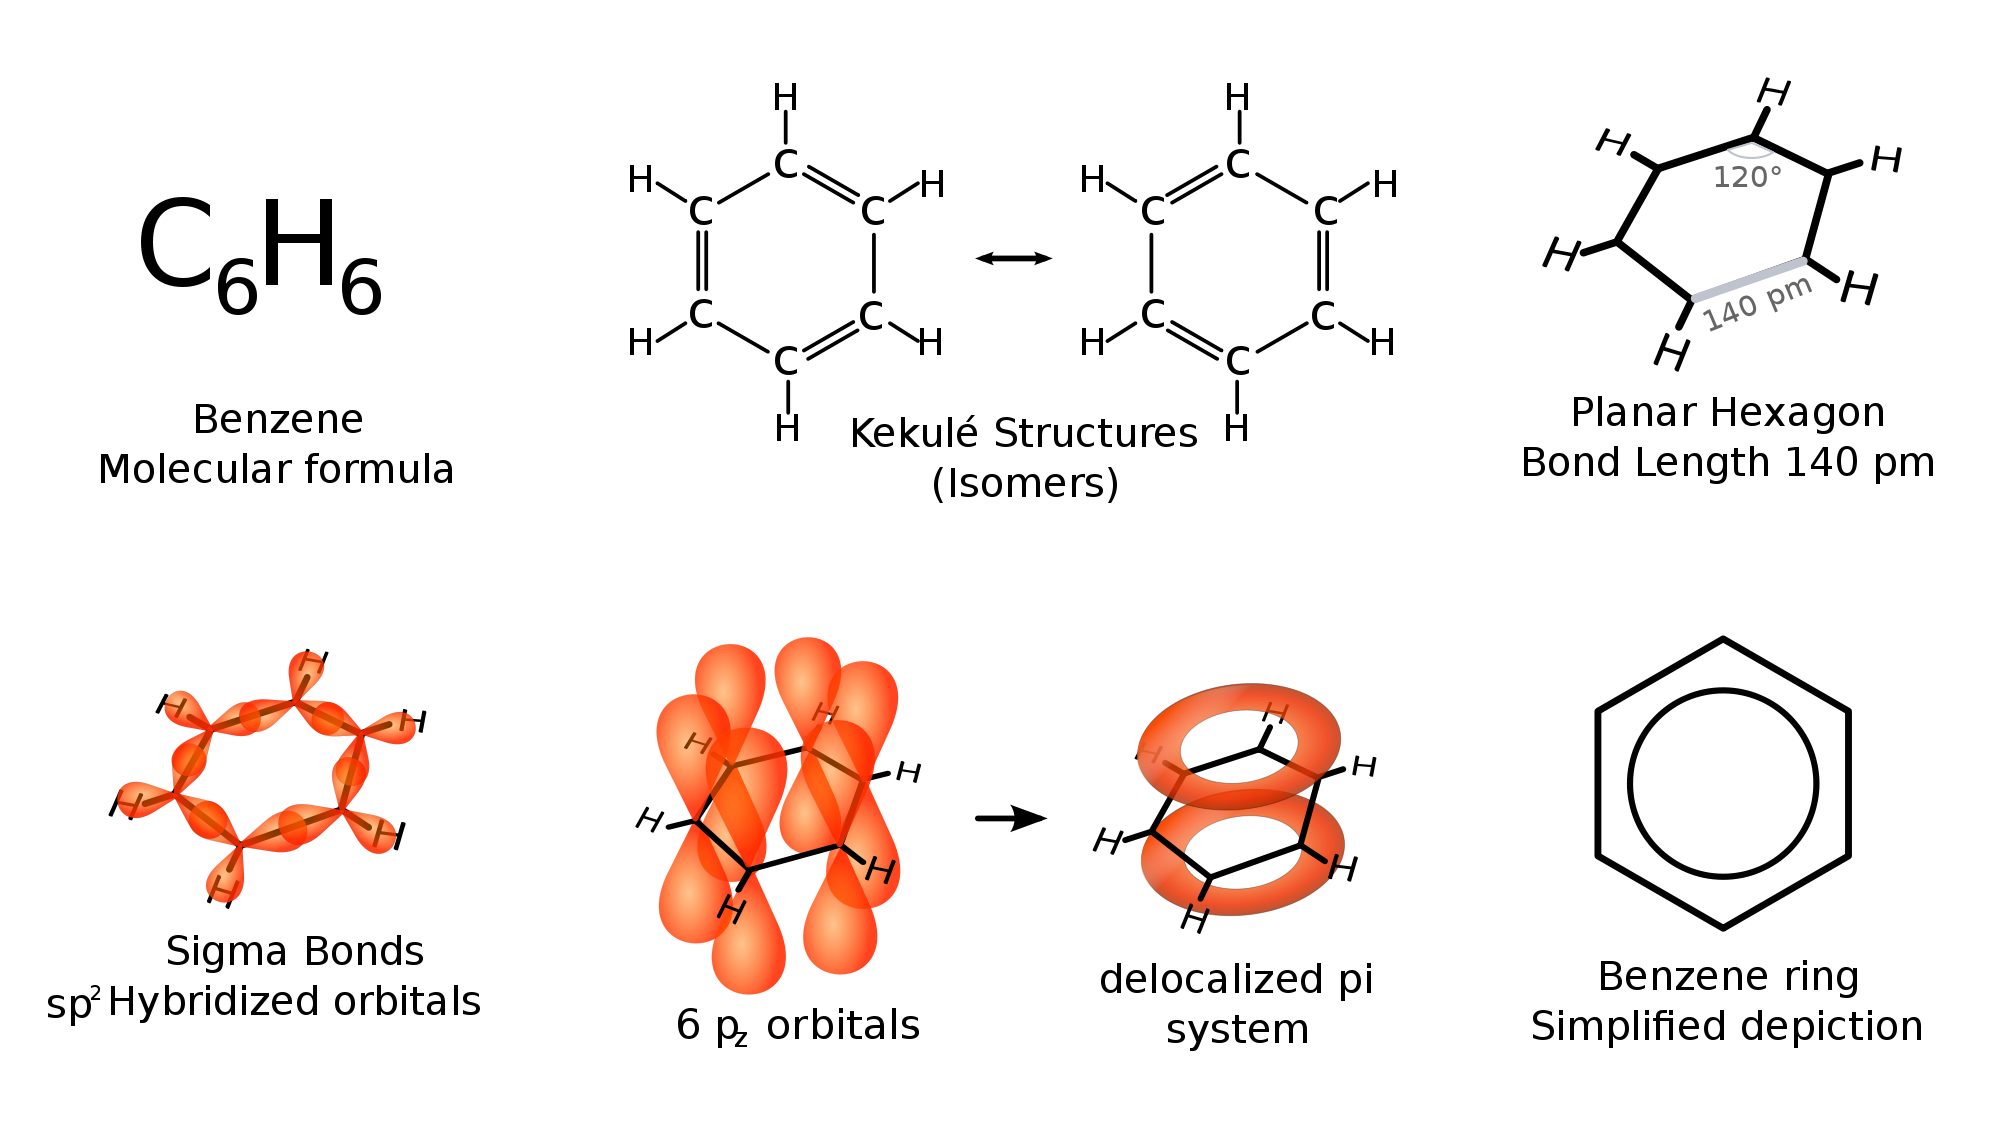
\includegraphics[width=1\linewidth]{imagens/benzeno_detalhes.png}
\end{figure}

Repare que tudo isso está presente no benzeno e devemos deixar bem claro que o \emph{sistema deslocalizado} presente na figura só existe por causa dos 6 orbitais p que formam as três ligações duplas presentes na molécula.

Claro, existem moléculas diferentes do benzeno que também apresentam aromaticidades, e não são poucas. Responda rápido: a piridina, mostrada a seguir, na figura \ref{fig:piridina}, é aromática ou não?

\begin{figure}[h]
	\centering
	\caption{Piridina: átomos pequenos = H, átomos ligados aos H = carbono, o restante = N}
	\label{fig:piridina}
	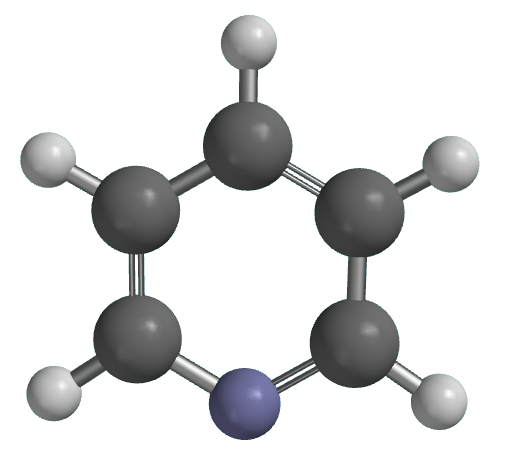
\includegraphics[width=0.45\linewidth]{imagens/pyridine03.png}
\end{figure}

A piridina é considerada uma molécula aromática devido à sua estrutura e propriedades que se encaixam nos critérios da teoria de aromaticidade, que foi desenvolvida inicialmente por Friedrich August Kekulé e Archibald Scott Couper e posteriormente refinada por outros químicos, como Linus Pauling e Robert S. Mulliken.

Os critérios que tornam uma molécula aromática incluem:

1. Planaridade: As moléculas aromáticas tendem a ser planares, o que significa que seus átomos estão dispostos no mesmo plano. A piridina atende a esse critério, pois os átomos de carbono e nitrogênio estão ligados de forma planar.

2. Anel conjugado: A aromaticidade geralmente envolve um sistema de anel conjugado, no qual os átomos de carbono (ou outros átomos) estão ligados alternadamente com ligações simples e duplas (ou ressonantes). Na piridina, o anel de seis membros contém cinco átomos de carbono e um átomo de nitrogênio, com ligações simples e duplas alternadas, formando um sistema conjugado.

3. Número ímpar de pares de elétrons {$\pi$}: Em moléculas aromáticas, o número de pares de elétrons {$\pi$} no sistema de anel conjugado deve ser ímpar. Isso significa que deve haver um número ímpar de elétrons {$\pi$} deslocalizados no sistema. Na piridina, o anel contém 6 elétrons {$\pi$}, ou três pares, satisfazendo esse critério.

4. Estabilidade: Moléculas aromáticas são altamente estáveis devido à sua estrutura eletrônica especial. Essa estabilidade resulta em uma menor reatividade em relação a adições químicas típicas, como a adição de hidrogênio em uma reação de hidrogenação.


%###########################################################################################
\chapter{Introdução às funções orgânicas}
\begin{mdframed}[backgroundcolor=orange!20,linewidth=0pt,roundcorner=10pt]
	\minitoc
\end{mdframed}
As funções orgânicas são grupos de compostos químicos que compartilham características estruturais e propriedades químicas semelhantes. Elas desempenham um papel fundamental na Química Orgânica, que é o ramo da Química que se concentra no estudo dos compostos que contêm carbono. Os compostos orgânicos podem ser encontrados em uma variedade impressionante de formas e tamanhos, e as funções orgânicas são a maneira pela qual os químicos classificam e compreendem essa diversidade.

As funções orgânicas são essenciais para entender a química dos compostos orgânicos e desempenham um papel crucial em muitos aspectos da química, incluindo a síntese de produtos químicos, a bioquímica, a farmacologia e a indústria química. Esta introdução pretende explorar algumas das funções orgânicas mais comuns e destacará sua importância no estudo da Química Orgânica e na vida cotidiana.


\section{Reconhecimento de padrões}
Faça um exercício mental simples: você consegue separar os bilhões de seres humanos que habitam o planetinha azul chamado Terra de acordo com alguma característica? Analisando friamente, percebemos diferenças no formato dos olhos, na pigmentação da pele, no formato dos cabelos, entre tantas outras características. Se você agrupou alguns humanos, você provavelmente chegou perto de uma etnia. Paramos por aqui com humanos.

Igualmente, se você decidir agrupar automóveis segundo, por exemplo, a potência do motor, número de portas ou qualquer outra característica, você criou uma categoria automobilística.

Este exercício pode ser repetido com músicas, livros, filmes computadores, celulares, ou números, entre tantos outros possíveis elementos que podem ser agrupados.

Fácil, certo?

Sim, desde que você defina alguma característica que diferencie um grupo de outro e coloque junto entidades com características semelhantes.

Antes de tratarmos de moléculas orgânicas, você precisa acostumar seu cérebro naquilo que é conhecido como \textbf{"Reconhecimento de Padrões"}. Veja como nem sempre é simples. oi

\begin{table}[!h]
	\begin{center}
	\caption{\label{padroes}Exercício simples sobre reconhecimento de padrões}
	\vspace{0.5cm}
	\begin{tabular}{|c | c | c|}
	\hline
	4 & 15 & 5\\
	\hline
	5 & 24 & 8\\
    \hline
	2 & 3 & 1\\
	\hline
    7 & \textbf{x} & 16\\
    \hline
	\end{tabular}
	\end{center}
\end{table}

Como você encontra o valor desconhecido apresentado na tabela \ref{padroes}? Existe um padrão que se repete em todas as linhas e caso o encontre nas três primeiras linhas, o valor de x quase que emerge de seu cérebro. 

Quanto tempo levou para encontrar o padrão, principalmente até se dar conta de que pode ignorar a coluna numérica da esquerda?

Independente do tempo gasto na resolução do problema, o padrão escondido nos números é bem simples: os valores numéricos da coluna central são \textbf{o triplo} dos valores da coluna numérica da direita. Assim, o valor de x deve ser o triplo de 16, ou seja, 48.

Existe um outro aspecto que deve ser considerado neste ponto de nossa análise sobre funções orgânicas: a similaridade. De modo bem simplificado, podemos admitir que similaridade está muito relacionada com semelhança e assim podemos dizer que a entidade A é similar à entidade B se vários elementos presentes em A também estejam presentes na entidade B.

Considere a Figura \ref{fig:carros} a seguir. Nela podemos visualizar um conjunto de desenhos com a parte dianteira de alguns automóveis fictícios.

\begin{figure}[h]
	\centering
	\caption{Representação de alguns automóveis.}
	\vspace{0.5cm}
	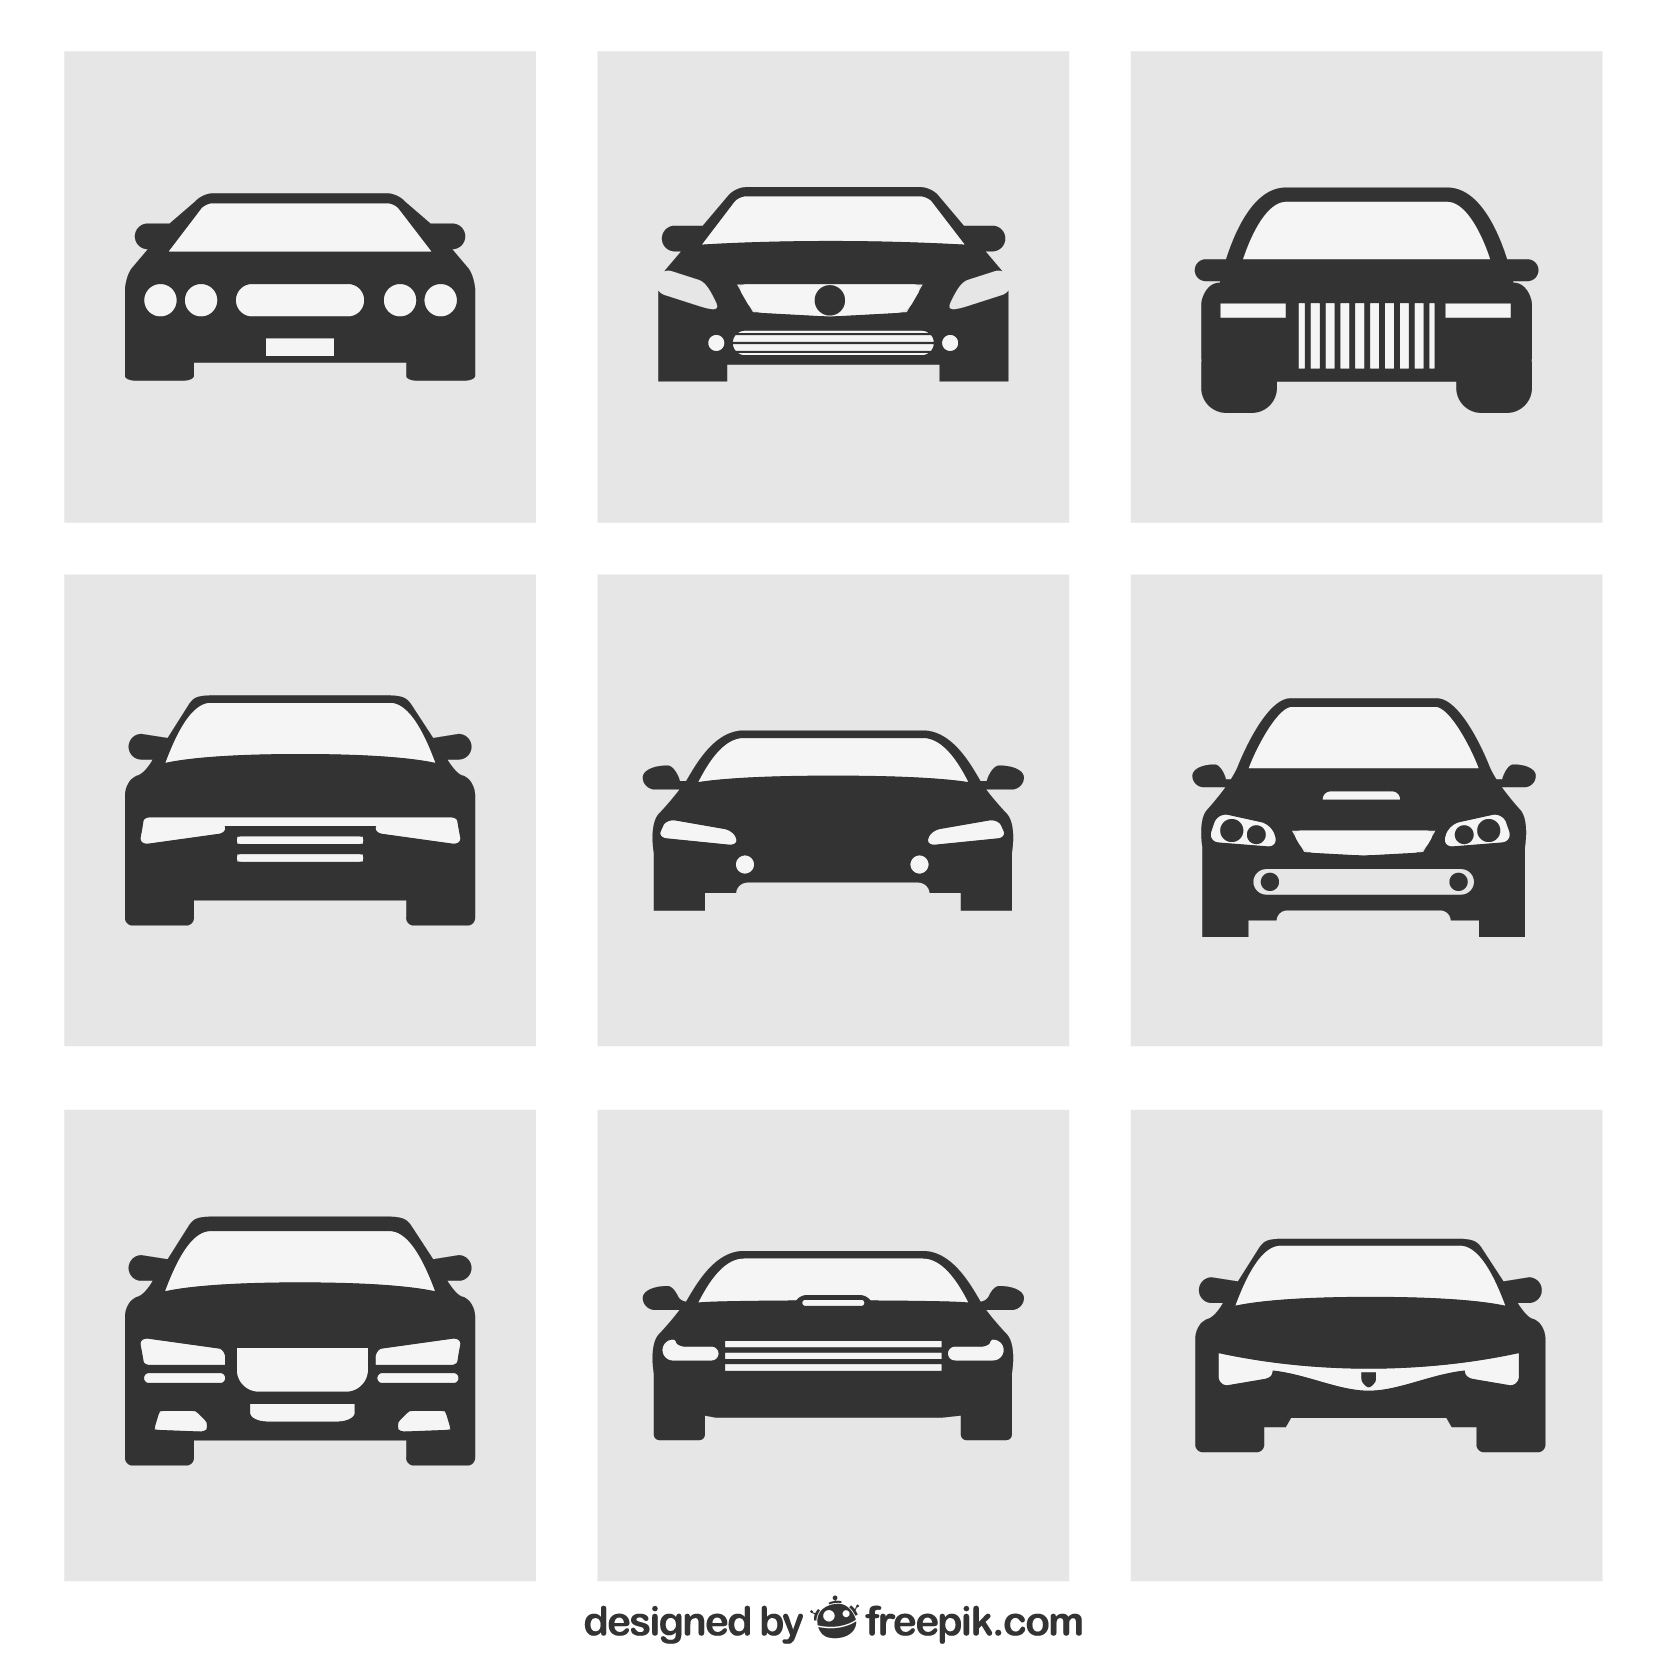
\includegraphics[width=0.5\linewidth]{imagens/19035-NRYBNX.jpg}
    \caption*{Fonte: https://shorturl.at/crzG0}
	\label{fig:carros}
\end{figure}

A Figura \ref{fig:carros} neste contexto ajuda a praticar a busca por similaridade em imagens, algo que será muito útil quando precisarmos identificar todas as funções orgânicas presentes em uma molécula polifuncional, pois uma destas funções deve ser a chamada "sênior" ou "principal" para que possamos montar o seu nome a partir de sua estrutura.

Quais elementos tornam as seis partes da imagem representada na figura similares entre si? Podemos visualizar alguns elementos presentes em todas as imagens:

\begin{itemize}
	\item Duas rodas visíveis.
	\item Dois espelhos retrovisores
	\item Um para-brisa
\end{itemize}

Repare que os faróis dos automóveis não são idênticos, assim como as grades frontais também são distintas. Assim, as representações dos automóveis são similares em algum aspecto.

%########################
\section{Função orgânica}
O mesmo ocorrerá quando precisarmos analisar uma estrutura orgânica complexa em busca das funções orgânicas presentes. Veja a molécula representada na Figura \ref{fig:vanco} a seguir.

\begin{figure}[h]
	\centering
	\caption{Estrutura da vancomicina}
	\vspace{0.5cm}
	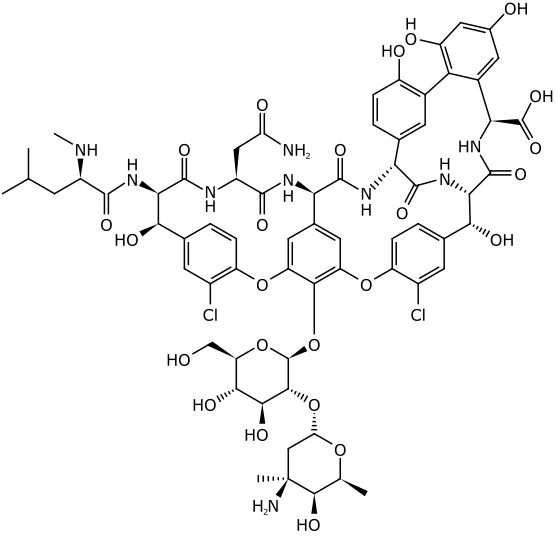
\includegraphics[width=0.85\linewidth]{imagens/557px-Vancomycin.svg}
	\caption*{Fonte: Wikipedia https://shorturl.at/nAZ01}
	\label{fig:vanco}
\end{figure}

Ainda sem analisar os detalhes de cada função orgânica presente na vancomicina, uma substância classificada como antibiótico, percebe-se que existem alguns conjuntos de átomos que se repetem na estrutura, algo como (guardadas as devidas proporções) ocorre na Figura \ref{fig:carros}.

É relativamente fácil encontrar alguns desses grupos de átomos:

\begin{itemize}
	\item átomo de Oxigênio ligado a átomo de Hidrogênio;
	\item átomo de Nitrogênio ligado a dois átomos de Oxigênio;
	\item átomo de Carbono ligado a um átomo de Oxigênio por uma ligação covalente dupla.
\end{itemize}

Cada um desses conjuntos é uma \textbf{função orgânica}.

Existem dezenas delas, todas categorizadas, organizadas e designadas por seus nomes pela IUPAC, conforme pode ser analisado no IUPAC BlueBook \cite{iupac2013}.

O número de substâncias orgânicas conhecidas já ultrapassou a grandeza de dezenas de milhões, e métodos sintéticos novos geram ainda mais substâncias \cite{doi:10.1021/acs.jmedchem.2c00223}. Cada substância química precisa de um nome que caracterize sua unicidade e existem muitas regras para que cada uma delas tenha seu nome de maneira inequívoca.

A Figura \ref{fig:funcoes2} mostra um resumo das funções orgânicas que serão analisadas neste livro, contendo, além do nome, uma representação geral e também o sufixo correspondente.

\begin{figure}[h]
	\centering
	\caption{Resumo das funções orgânicas.}
	\vspace{0.5cm}
	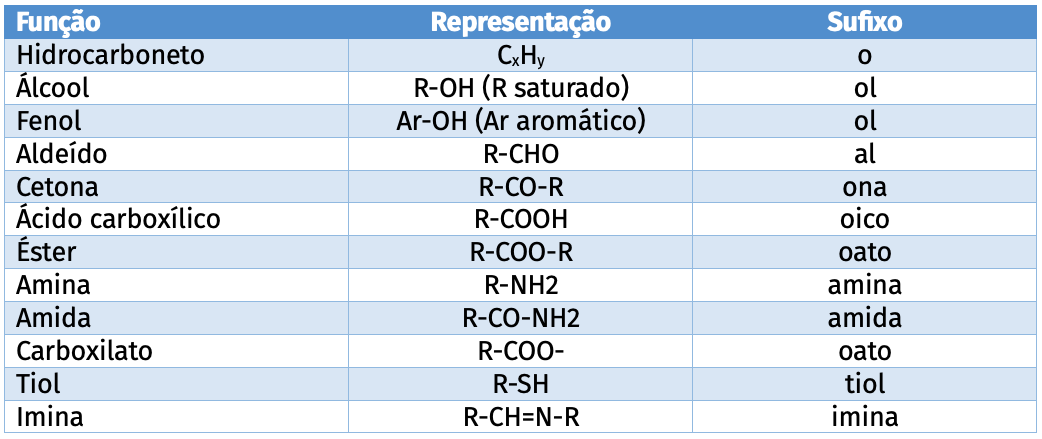
\includegraphics[width=1\linewidth]{imagens/funcoes.png}
	\caption*{Fonte: autores}
	\label{fig:funcoes2}
\end{figure}

%###################################


\chapter{Hidrocarbonetos}
Os hidrocarbonetos são uma classe fundamental de compostos químicos que desempenham um papel central na química orgânica. Eles consistem exclusivamente em átomos de carbono e hidrogênio, formando uma família diversificada de moléculas que variam desde as mais simples até as mais complexas. A simplicidade de sua composição, que consiste apenas em dois elementos, torna os hidrocarbonetos um dos grupos de compostos mais estudados e essenciais na química orgânica, e um exemplo destes pode ser visto na figura \ref{fig:ocatene}

\begin{figure}[H]\centering
\caption{Um hidrocarboneto encontrado no petróleo}
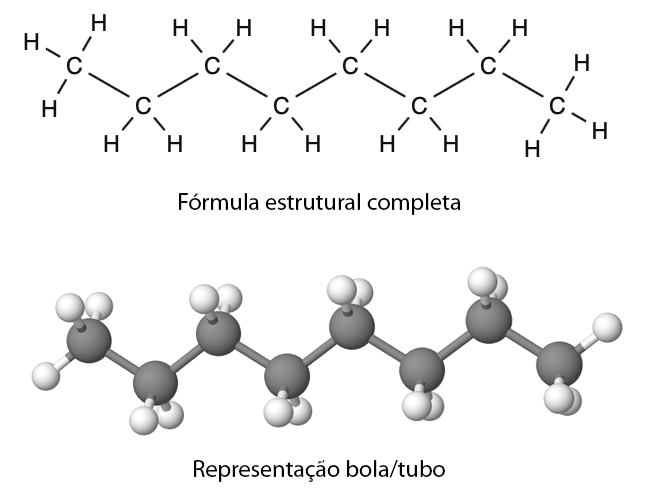
\includegraphics[scale=0.5]{imagens/octano.png}
\label{fig:ocatene}\vspace{0.5cm}\end{figure}

Algumas das características da representação estrutural presente na figura \ref{fig:ocatene} serão úteis em diversos outros momentos deste livro e podemos tratar sobre algumas delas. A imagem apresenta duas representações estruturais possíveis para o hidrocarboneto com nome oficial \textbf{octano}, com exatamente o mesmo significado, mas como aparência visual distinta. 

A representação na parte superior da imagem mostra todas as ligações covalentes (representadas por traços simples) presentes na molécula do octano e apresenta uma sugestão de como deve ser a formato espacial da molécula, considerando que todos os átomos de carbono são saturados e, portanto, possuem hibridização sp$^3$ e arranjo espacial tetraédrico, conforme analisado anteriormente. Mas uma representação mais precisa exige software específico para calcular todas as interações (atrativas e repulsivas) entre os átomos presentes na molécula e então chegar a uma estrutura com o menor valor energético possível. Mas por que? Menor valor energético está associado com maior estabilidade e menor reatividade, uma característica comum a todos os hidrocarbonetos.

A parte inferior da figura apresenta uma representação chamada de \textbf{bola/tubo}, onde os átomos são representados por bolas (de tamanhos e cores diferentes) e as ligações covalentes são representadas por tubos. Uma ligação covalente simples é representada por um único tubo, enquanto as ligações covalentes duplas e triplas são representadas por tubos duplos ou triplos, respectivamente.

Ainda na figura \ref{fig:ocatene}, todos os átomos de carbono encontram-se ligados por ligações covalentes simples, o que classifica essa sequência de átomos de carbono, a partir deste ponto chamada de \textbf{cadeia carbônica} como \textbf{cadeia saturada}. Caso a cadeia carbônica possua uma ligação covalente dupla entre o carbono da extremidade esquerda e seu vizinho imediato (neste exemplo), conforme pode ser visto na figura \ref{fig:hexene}, a cadeia passa a ser classificada como insaturada.

\begin{figure}[h]\centering
\caption{Um hidrocarboneto insaturado}
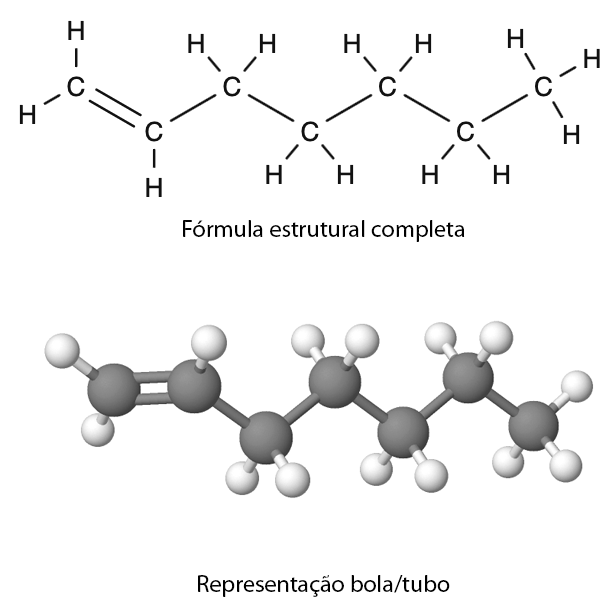
\includegraphics[scale=0.5]{imagens/hexeno.png}
\label{fig:hexene}\vspace{0.5cm}\end{figure}

Os hidrocarbonetos desempenham um papel vital em inúmeros aspectos da nossa vida cotidiana. Eles são os principais constituintes dos combustíveis fósseis, como petróleo e gás natural, que propulsionam nossos veículos e fornecem energia para a geração de eletricidade. Além disso, muitos produtos químicos, plásticos e materiais sintéticos são derivados de hidrocarbonetos.

Esta introdução explorará a estrutura básica dos hidrocarbonetos, suas diferentes categorias e sua relevância em várias aplicações, desde o setor energético até a indústria química e farmacêutica, destacando sua importância na química orgânica e na nossa sociedade moderna.
\section{Origens do petróleo}
A teoria orgânica para a origem do petróleo é uma das explicações mais aceitas para a formação desse recurso natural. Ela postula que o petróleo se origina a partir da decomposição de matéria orgânica, como plantas e microorganismos, ao longo de milhões de anos sob condições específicas de pressão e temperatura no subsolo. Esta teoria foi proposta pela primeira vez no século XIX e é conhecida como a teoria biogênica.

A \textbf{teoria orgânica} descreve o processo de formação do petróleo da seguinte maneira:

1. Acúmulo de Matéria Orgânica: No passado geológico, oceanos e lagos continham uma grande quantidade de matéria orgânica em diferentes estados de decomposição, incluindo plâncton, algas e outros resíduos biológicos. Toda essa matéria orgânica se acumulava no fundo dessas águas, onde a falta de oxigênio limitava a decomposição completa.

2. Sepultamento: Com o tempo, sedimentos foram se acumulando sobre a matéria orgânica, causando seu sepultamento no subsolo. Essa incrível sobreposição de sedimentos exerceu pressão sobre a matéria orgânica, comprimindo-a.

3. Aumento de Temperatura e Pressão: À medida que os sedimentos continuaram a se acumular, a temperatura e a pressão no subsolo aumentaram gradualmente. A essa profundidade, a matéria orgânica passou por uma série de transformações químicas conhecidas como diagênese. Durante esse processo, a matéria orgânica se transformou em uma mistura complexa de hidrocarbonetos.

4. Migração e Armazenamento: Os hidrocarbonetos resultantes do processo de diagênese migraram através de rochas porosas e segmentos impermeáveis em direção às camadas superiores. Eles eventualmente ficaram presos em bolsas subterrâneas, formando reservatórios de petróleo.

5. Processo de Maturação: Com o tempo, os hidrocarbonetos continuaram a sofrer mudanças químicas, refinando-se e produzindo petróleo bruto, gás natural e outros componentes. A qualidade e a composição do petróleo podem variar dependendo das condições geológicas locais.

É importante observar que a teoria orgânica não é a única explicação para a origem do petróleo. Existem outras teorias, como a teoria abiótica, que sugere que o petróleo pode ser formado a partir de processos químicos não relacionados à matéria orgânica. No entanto, a teoria orgânica é amplamente aceita e tem uma base sólida na geologia e na química orgânica. Ela também se alinha com a grande quantidade de evidências geológicas e experimentais coletadas ao longo de muitas décadas.

A teoria inorgânica para a origem do petróleo é uma explicação alternativa à teoria orgânica predominante. Enquanto a teoria orgânica postula que o petróleo se forma a partir da decomposição de matéria orgânica, como micro-organismos marinhos e plantas terrestres, a teoria inorgânica sugere que o petróleo pode se originar de processos não relacionados a organismos vivos.

A \textbf{teoria inorgânica} propõe que o petróleo é formado por reações químicas no interior da Terra, envolvendo elementos inorgânicos, como carbono, hidrogênio e nitrogênio. Os defensores dessa teoria argumentam que o petróleo é encontrado em profundidades muito maiores do que seria esperado se fosse proveniente de restos orgânicos, e que os processos geológicos e químicos subterrâneos podem produzir hidrocarbonetos a partir de substâncias não orgânicas.

Uma das principais hipóteses dentro da teoria inorgânica é a abiótica, que sugere que o petróleo é produzido por reações químicas de alta pressão e temperatura no manto da Terra, muito abaixo da camada onde a matéria orgânica é encontrada. Essas reações envolvem a transformação de minerais ricos em carbono, como calcário e magnésio, em hidrocarbonetos.

No entanto, é importante destacar que a teoria inorgânica enfrenta desafios significativos e não é amplamente aceita na comunidade científica. A teoria orgânica tem uma base sólida de evidências geológicas, juntamente com evidências geoquímicas e paleontológicas que apoiam a origem orgânica do petróleo. Além disso, a teoria inorgânica ainda não conseguiu explicar completamente a diversidade de compostos encontrados no petróleo cru.

\section{Classificação}
A classificação de hidrocarbonetos é um tópico fundamental na química orgânica, uma vez que os hidrocarbonetos constituem a base de muitos compostos orgânicos. Os hidrocarbonetos são compostos formados exclusivamente por átomos de carbono (C) e hidrogênio (H) e podem ser categorizados de acordo com a natureza das ligações entre os átomos de carbono e sua estrutura geral. Existem três grandes  categorias principais de hidrocarbonetos: alcanos, alcenos e alcinos, cada uma com características distintas.

1. \textbf{Alcanos}: são hidrocarbonetos que possuem apenas em ligações simples (ligações sigma) entre os átomos de carbono. Eles são conhecidos como hidrocarbonetos saturados, pois apresentam a máxima quantidade possível de hidrogênios. A fórmula geral dos alcanos é C{$_n$}H$_{(2n+2)}$, onde "n" representa o número de átomos de carbono na cadeia. Exemplos de alcanos incluem o metano (\ce{CH4}), o etano (\ce{C2H6}), o propano (\ce{C3H8}) e o butano (\ce{C4H10}). Alcanos têm pontos de ebulição mais baixos e são geralmente menos reativos em comparação com outras classes de hidrocarbonetos.

\begin{figure}[h]\centering
\caption{Um exemplo de hidrocarboneto do tipo alcano, com fórmula molecular \ce{C8H18}}
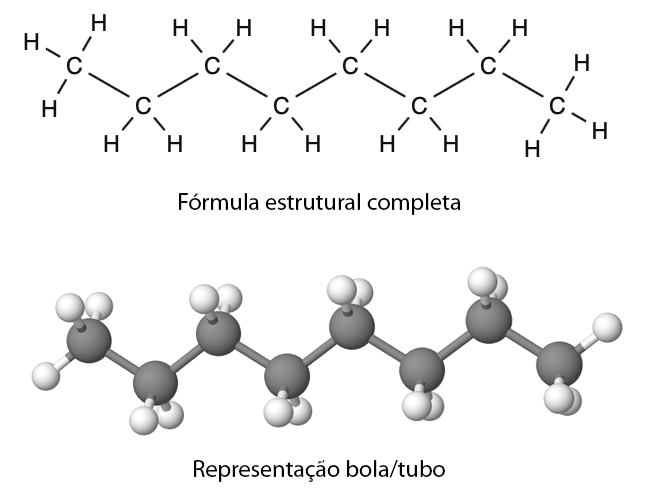
\includegraphics[scale=0.5]{imagens/octano.png}
\label{fig:alcano}\vspace{0.5cm}\end{figure}

2. \textbf{Alcenos}:
Os alcenos são hidrocarbonetos que contêm pelo menos uma ligação dupla (ligação pi) entre átomos de carbono na cadeia. A fórmula geral dos alcenos é CnH2n, onde "n" representa o número de átomos de carbono na cadeia. A presença da ligação dupla introduz uma insaturação na molécula. Exemplos de alcenos incluem o eteno (\ce{C2H4}), o propeno (\ce{C3H6}) e o buteno (\ce{C4H8}). Os alcenos tendem a ser mais reativos do que os alcanos devido à presença da ligação dupla, que permite a ocorrência de reações de adição.

3. \textbf{Alcinos}:
Os alcinos são hidrocarbonetos que contêm pelo menos uma ligação tripla (duas ligações pi e uma ligação sigma) entre átomos de carbono na cadeia. A fórmula geral dos alcinos é C{$_n$}H$_{(2n-2)}$, onde "n" representa o número de átomos de carbono na cadeia. A ligação tripla torna os alcinos ainda mais reativos do que os alcenos e alcanos. Exemplos de alcinos incluem o etino (\ce{C2H2} e o propino (\ce{C3H4}). Devido à sua alta reatividade, os alcinos são frequentemente usados como intermediários em sínteses orgânicas.

Além dessa classificação básica, os hidrocarbonetos também podem ser classificados com base na sua estrutura ramificada ou cíclica:

1. \textbf{Ramificados}:

Hidrocarbonetos podem apresentar grupos alquilas, também ligados à cadeia principal. A presença de destas leva à formação de isômeros, que são compostos com a mesma fórmula molecular, mas com diferentes arranjos espaciais. Os isômeros podem ter propriedades químicas e físicas distintas.

\begin{figure}[h]\centering
\caption{Um exemplo de hidrocarboneto ramificado, chamado 2,2-dimetil-propano}
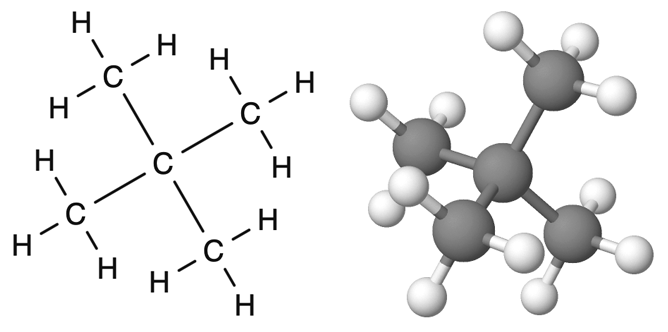
\includegraphics[scale=0.35]{imagens/neopentano.png}
\label{fig:ramificado}\vspace{0.5cm}\end{figure}

Na figura \ref{fig:ramificado}, átomos de carbono são representados por bolas de cor escura e átomos de hidrogênio são as bolas mais claras, e os tubos que conectam as bolas representam ligações covalentes simples, neste exemplo.

2. \textbf{Cíclicos}:

Muitos hidrocarbonetos formam ciclos ou anéis em suas estruturas. Esses compostos são chamados de hidrocarbonetos cíclicos. O ciclo mais simples é o ciclopropano, composto por um anel de três carbonos. Cicloexano, ciclopentano e ciclobutano são outros exemplos de hidrocarbonetos cíclicos.

\begin{figure}[h]\centering
\caption{Representação do cicloexano nas notações \textbf{fórmula estrutural completa e bola/tubo}}
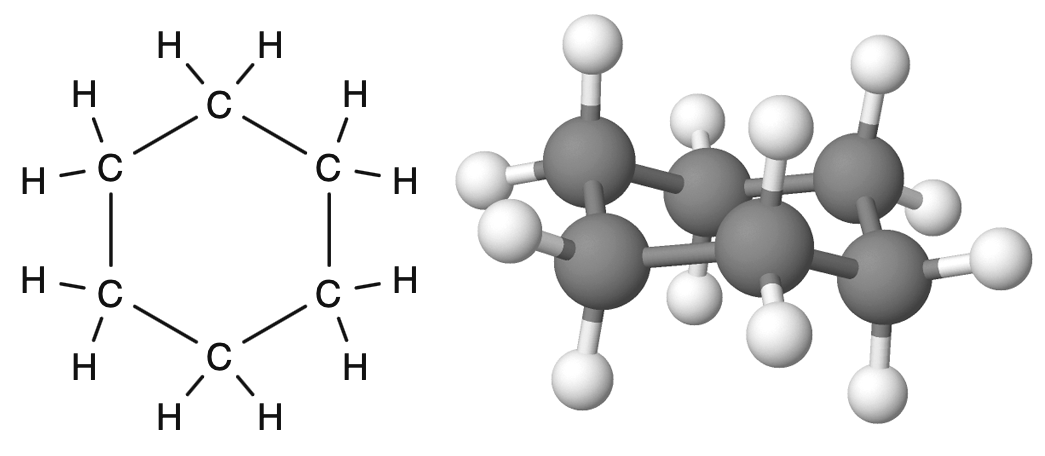
\includegraphics[scale=0.35]{imagens/cicloexano.png}
\label{fig:cicloexano}\vspace{0.5cm}\end{figure}

A figura \ref{fig:cicloexano} apresenta um dos mais belos e complexos temas da Química Orgânica: os fundamentos da análise conformacional \cite{carey2022organic}. Analisar a forma tridimensional de uma molécula é fundamental para compreender sua interação com outras moléculas ou então com substratos biológicos. 

Uma pergunta é absolutamente válida neste momento: por qual razão a molécula do ciclo-hexano, visualizada à direita na figura \ref{fig:cicloexano} não é plana? Conforme dito anteriormente, o uso de algum software específico para cálculo do melhor arranjo tridimensional de uma molécula como a do ciclo-hexano produz uma saída como a mostrada na figura \ref{fig:cicloexano}.

A explicação é simples: os seis átomos  de carbono do ciclo-hexano são todos \textbf{saturados} e, por causa da hibridização sp$^3$, todos os orbitais híbridos estão separados entre si por uma distância angular de 109,5$^o$. Esse arranjo espacial, denominado \textbf{tetraédrico}, obriga o conjunto todo a organizar-se tridimensionalmente no formato exibido à direita da figura \ref{fig:cicloexano}. A representação da esquerda, sugerindo um arranjo planar, é uma muito grande simplificação do arranjo correto, mas adequada para fins didáticos.

Além dessas categorias, a aromaticidade é uma propriedade especial observada em alguns hidrocarbonetos, como o benzeno. Moléculas consideradas aromáticas apresentam uma estabilidade excepcional devido ao fenômeno conhecido por ressonância eletrônica em seu sistema de anel, tornando-as distintas das categorias mencionadas anteriormente.

A classificação de hidrocarbonetos é essencial na química orgânica, pois ajuda os químicos a compreenderem a estrutura, as propriedades e o comportamento desses compostos. Além disso, a capacidade de categorizar os hidrocarbonetos facilita a previsão de suas reações químicas e aplicações em diversas áreas, como indústria, farmácia e pesquisa científica. 

\section{Propriedades físicas de hidrocarbonetos}
Hidrocarbonetos são substâncias formadas apenas por átomos e carbono e átomos de hidrogênio, constituindo a espinha dorsal que pode originar muitas moléculas encontradas na natureza. Podem ser classificados em várias categorias, e suas propriedades físicas são importantes para compreender suas reações em condições naturais e industriais.

\subsection{Pontos de Fusão e Ebulição}

Os pontos de fusão dos hidrocarbonetos são afetados preferencialmente pelo número de átomos de carbono em suas moléculas e pelo arranjo topológico e espacial entre esses átomos. Os hidrocarbonetos classificados como saturados, como os alcanos, tendem a apresentar pontos de ebulição mais baixos, enquanto alcenos e alcinos (insaturados com ligação dupla ou tripla, respectivamente) tendem a apresentar pontos de ebulição mais elevados. A razão do aumento nos valores de PF é simples: sendo apolares, as moléculas dos hidrocarbonetos atraem-se por meio das chamadas Forças de London, tipicamente fracas, mas à medida em que o número de átomos de carbono aumenta, tal atração torna-se acumulativamente mais significante e, portanto, os valores de PF aumentam. Veja um exemplo na tabela \ref*{pf} a seguir.

\begin{table}[!h]
\begin{center}
\caption{\label{pf}Temperaturas de fusão e ebulição de alguns hidrocarbonetos saturados.}
\vspace{0.5cm}
\begin{tabular}{|c|c|c|c|c|}
\hline
Substância & Fórmula & Massa molar (g/mol) & TF ({$^o$}C) & TE ({$^o$}C)\\
\hline
Metano & \ce{CH4} & 16 & -182 & -161 \\
\hline
Etano & \ce{C2H6} & 30 & -183 & -87 \\
\hline
Propano & \ce{C3H8} & 44 & -188 & -42 \\
\hline
Butano & \ce{C4H10} & 58 & -138 & -0,5 \\
\hline
Pentano & \ce{C5H12} & 72 & -130 & -36 \\
\hline
\end{tabular}
\end{center}
\end{table}

Os pontos de ebulição dos hidrocarbonetos estão intimamente relacionados com o tamanho e a forma das moléculas. Por tal razão, dois hidrocarbonetos isômeros de cadeia (moléculas com mesma fórmula molecular, mas com cadeias carbônicas distintas), pentano e 2,2-dimetil-propano possuem Ponto de Ebulição tão distintos. A cadeia carbônica do pentano é normal (sem ramificações), enquanto a cadeia carbônica do 2,2-dimetil-propano é ramificada, o a faz tender a um formato esférico, com menor área superficial que o pentano. Assim, as forças de atração no poentano se tornam maiores e os PF são tão distintos, conforme pode ser visto na figura \ref{fig:pentano} a seguir.

\begin{figure}[h]
	\centering
	\caption{Influência da forma da molécula nos valore de PE}
	\vspace{0.5cm}
	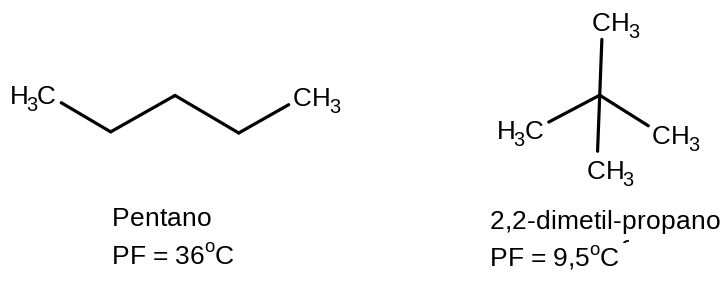
\includegraphics[width=1\linewidth]{imagens/pentano_22dimetil.png}
\label{fig:pentano}
\end{figure}


\subsection{Solubilidade}

A solubilidade dos hidrocarbonetos em água é geralmente muito baixa devido à natureza apolar de suas moléculas. No entanto, a solubilidade pode aumentar ligeiramente com o tamanho da cadeia carbônica, pois moléculas maiores possuem área superficial maior para interagir com as moléculas de água, mas isso só ocorre em poucas situações, como emulsões ou então quando óleo (mistura complexa de hidrocarbonetos) flutua na água.

A solubilidade é uma característica importante para a separação de hidrocarbonetos em processos de refino de petróleo e na indústria química. Sendo moléculas apolares, os hidrocarbonetos tendem a dissolver-se em moléculas igualmente apolares e, portanto, tendem a não interagir com água. Porém, dissolvem-se bem em solventes igualmente apolares, como benzeno (\ce{C6H6}).

De modo geral, hidrocarbonetos de cadeias curtas são mais solúveis em solventes apolares do que hidrocarbonetos de cadeia carbônica maior, pois moléculas menores podem dispersar-se melhor entre as moléculas do solvente. A ramificação das cadeias carbônicas dos hidrocarbonetos pode aumntar sua solubilidade em solventes apolares, uma vez que a área superficial é reduzida e uma molécula compacta dispersa-se melhor que uma molécula maior.

\subsection{Densidade}
A densidade de hidrocarbonetos varia com sua composição e estrutura molecular. Normalmente, os HC mais leves, como metano (\ce{C4}) ou etano (\ce{C2H6}) são menos densos que o ar, são inflamáveis e tendem a ascender, uma vez que todo gás menos denso que o ar sofre esse fenômeno. A densidade é uma característica  importante em processos de separação, como a destilação, através da qual os componentes são separados com base em suas diferenças de densidade. De modo geral, quanto maior a massa molar de um hidrocarboneto, maior será sua densidade, uma vez que uma molécula mais pesada apresenta maior massa por unidade de volume. Como exemplo, o propano (\ce{C3H8}) apresenta densidade com valor \textbf{0,498 g/mL} enquanto o decano (\ce{C10H22}) apresenta densidade com valor \textbf{0,730 g/mL} na mesma temperatura de 20{$^o$}C.

\subsection{Tensão Superficial}
Em uma amostra de água, existem dois tipos de moléculas. As que estão por fora, exteriores, e as que estão por dentro, interiores. As moléculas interiores são atraídas por todas as moléculas ao seu redor, enquanto as moléculas exteriores são atraídas apenas pelas outras moléculas da superfície e por aquelas abaixo da superfície. Isto faz com que o estado energético das moléculas no interior seja muito inferior ao das moléculas no exterior. Por causa disso, as moléculas tentam manter uma área superficial mínima, permitindo assim que mais moléculas tenham um estado de energia mais baixo. Isto é o que cria o que é conhecido como tensão superficial.

Em hidrocarbonetos, temos o mesmo comportamento, mas considerando as diferenças estruturais entre água e hidrocarbonetos. De forma geral, a tensão superficial aumenta com o aumento da massa molar do hidrocarboneto. Como exemplo, a substância conhecida como hexano (\ce{C6H14}) apresenta tensão superficial com valor 0,018 N/m, enquanto a água apresenta tensão superficial com valor 0,0720 N/m, quatro vezes maior que o hexano.

A figura \ref{fig:ts} ilustra como as moléculas normalmente se organizam em fase líquida e mostra de modo simplificado como as forças atrativas ajudam a criar a rede superficial de moléculas.

\begin{figure}[h]
	\centering
	\caption{Composição de forças para a criação da Tensão Superficial}
	\vspace{0.5cm}
	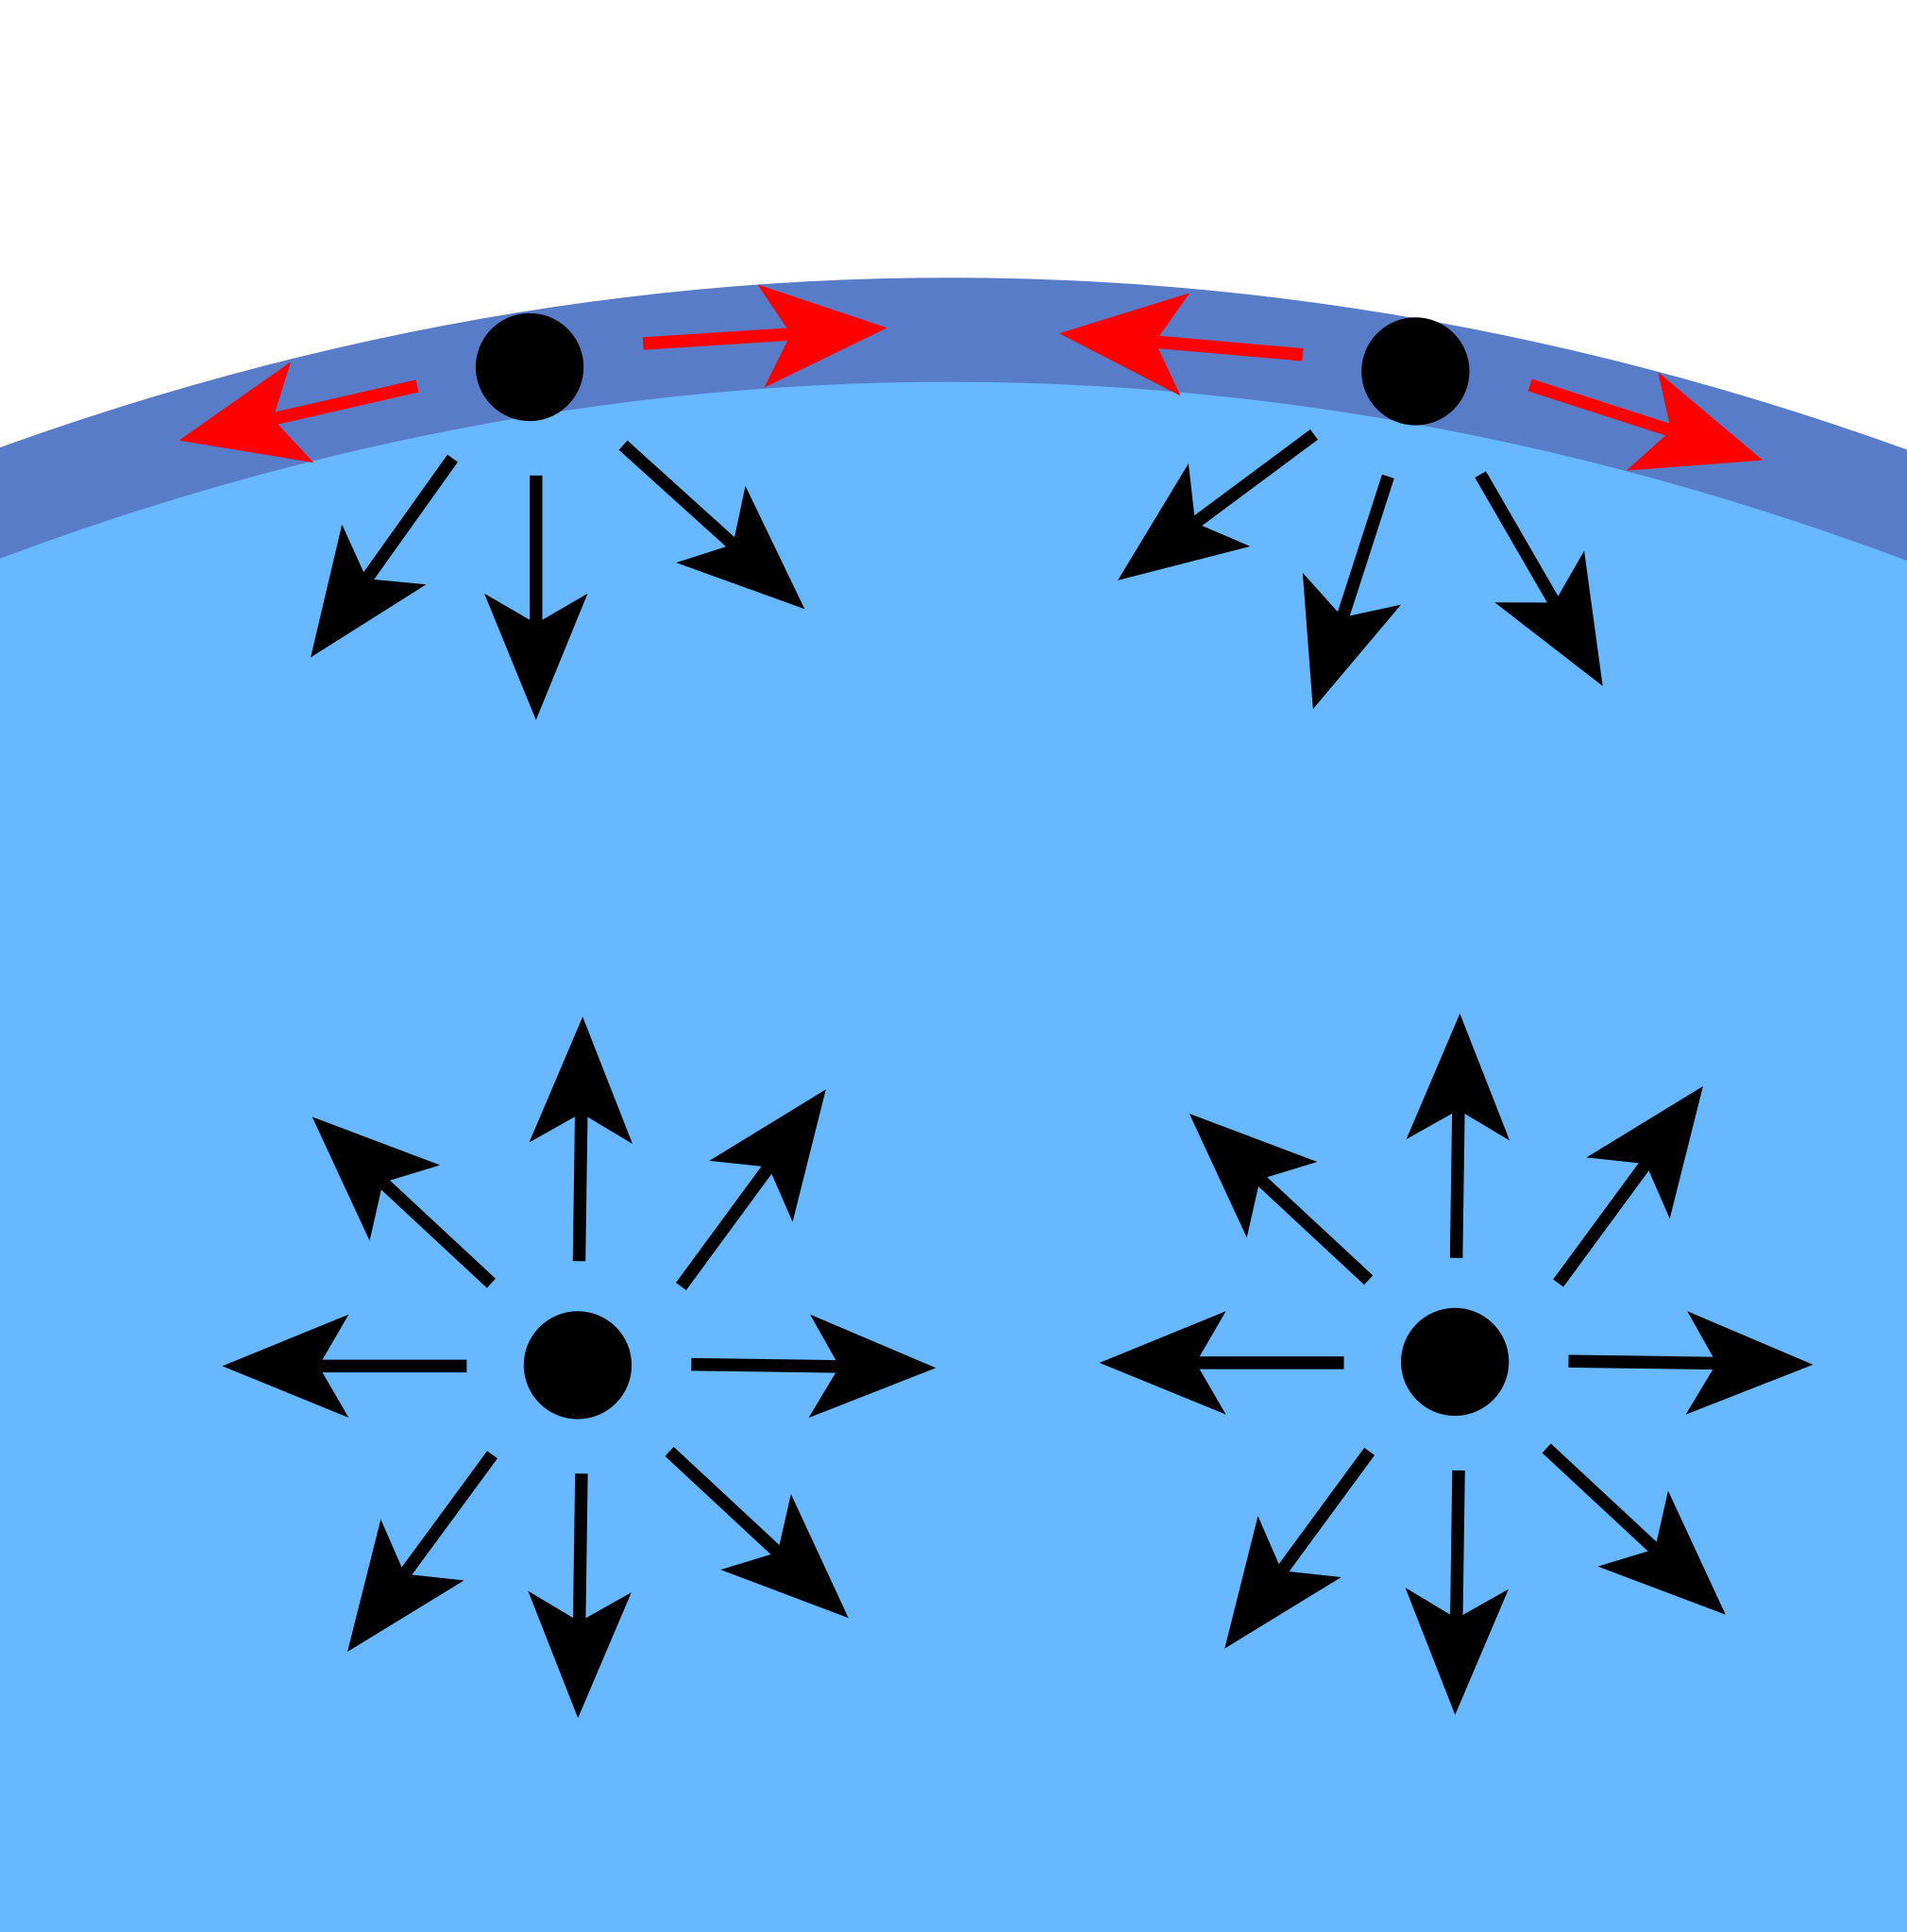
\includegraphics[width=1\linewidth]{imagens/ts.png}
\label{fig:ts}
\end{figure}

\section{Nomenclatura de hidrocarbonetos}
Assim como qualquer outra substância, todo hidrocarboneto precisa de ao menos dois conjuntos de informação: (a) uma fórmula que caracteriza suas propriedades e (b) um nome que define sua unicidade. Uma vez que são conhecidos centenas de milhares de hidrocarbonetos distintos, torna-se obrigatório o uso de alguma sistematização para criação de nomes únicos.

Esta imensa tarefa está centralizada na entidade conhecida como IUPAC (International Union for Pure and Applied Chemistry, ou União Internacional para Química Pura e Aplicada) e está registrada no chamado "BlueBook", documento específico para nomenclatura de substâncias orgânicas.

Devemos alertar o leitor que, uma vez que são conhecidas milhões de substâncias orgânicas, a quantidade de regras e orientações sugeridas pela IUPAC é relativamente grande e abordaremos neste documento, aos poucos, parte dessas regras, pois nossa obra tem escopo bem definido não necessita de todas as regras. Deixamos aqui a curiosidade do leitor na leitura das regras previstas na versão 3 do BlueBook.

\subsection{Nomenclatura substitutiva}
Este é o principal método utilizado para nomenclatura de substâncias orgânicas e, mais amplamente, para substâncias que possuam elementos dos grupos 13 a 17 da Classificação Periódica dos Elementos. De modo geral, uma substância orgânica tem seu nome construído a partir de regras sistemáticas para que cada nome seja inequívoco, utilizando ao menos dois elementos:

\begin{description}
	\item \textbf{Hidreto pai ou cadeia principal}: é uma substância formada apenas por uma dada cadeia carbônica, sem qualquer grupo funcional, seja com cadeia normal, ramificada, cíclica, aromática ou ainda heterogênea, conforme pode ser observado na figura \ref{fig:hp} a seguir.
	
	\begin{figure}[h]
		\centering
		\caption{Exemplos de hidretos pai}
		\vspace{0.5cm}
		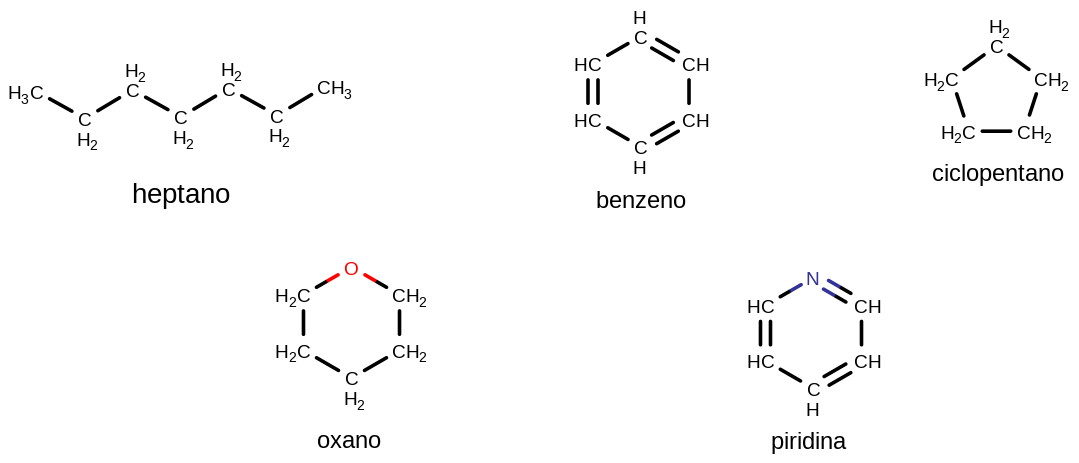
\includegraphics[width=1\linewidth]{imagens/hidretos_pai.png}
	\label{fig:hp}
	\end{figure}

	\item \textbf{Um grupo funcional principal}: caso a substância possua mais de um grupo funcional, um deles é o chamado \textbf{grupo funcional principal}, conforme pode ser visto na tabela \ref{senioridade} a seguir. As colunas "Prefixo" e "Sufixo" indicam, respectivamente, o nome de cada grupo funcional quando este não é a função principal (prefixo) e quando este é a função pricipal (sufixo).
\end{description}

Quando falamos da nomenclatura substitutiva, considere que um átomo de hidrogênio (por exemplo) tenha sido substituído por outro átomo o ou grupo de átomos.

\begin{table}[!h]
	%\begin{tabular}
	\begin{center}
	\caption{\label{senioridade}Grupos funcionais em ordem decrescente de senioridade (prioridade)}
	\vspace{0.5cm}
	\begin{tabular}{l c c c}
	\hline
	Função orgânica& Fórmula & Prefixo & Sufixo\\
	\hline
	Carboxilatos & \ce{-COO$^-$} & carboxilato & alcoxicarbonil\\
	Ácido carboxílico & \ce{-COOH} & ácido carboxílico & carboxi\\
	Ésteres & \ce{-COOR} & R-oato & R-oxicarbonil\\
	Haletos de acila & \ce{-COOX} & oil haleto & halocarbonil\\
	Amidas & \ce{-COONH2} & amida & carbamoil\\
	Nitrilas & \ce{-CN} & nitrila & ciano\\
	Aldeídos & \ce{-COH} & al & oxo\\
	Cetonas & \ce{-CO-} & ona & oxo\\
	Álcoois & \ce{-OH} & ol & hidroxi\\
	Tióis & \ce{-SH} & tiol & sulfanil\\
	Aminas & \ce{-NH2} & amina & amino\\
	Iminas & \ce{=NH} & imina & imino\\
	\hline
	\end{tabular}
	\end{center}
\end{table}

\begin{tcolorbox}[colback=blue!5!white,colframe=gray!75!black,title=Atenção!]
	Embora esta seção {\thesection} trate da nomenclatura de hidrocarbonetos, ficam lançadas as bases para a nomenclatura de muitas outras funções orgânicas. Este livro não cobre todas as funções orgânicas conhecidas por tratar-se de de uma obra de caráter básico, e o trabalho de criação das regras de nomenclatura orgânica estende-se há anos a certamente perdurará por outros ainda.
  \end{tcolorbox}




Caso o hidreto pai possua algum grau de insaturação (ligações duplas ou triplas), o sufixo do hidreto se altera para "eno" ou "ino", indicando as insaturações possível, com os localizadores adequados.

Naturalmente, a presença dos localizadores implica na necessidade da numeração da cadeia carbônica e, como consequência da presença de insaturação ou grupos funcionais, a numeração da cadeia igualmente segue regras bastante rígidas para manter a unicidade de cada nome.

A substância ilustrada abaixo, na figura \ref{fig:46} possui um nome construído pela nomenclatura substitutiva, onde átomos de hidrogênio foram substituídos de um dado hidreto pai.

\begin{figure}[h]
	\centering
	\caption{Exemplo de aplicação da nomenclatura substitutiva.}
	\vspace{0.5cm}
	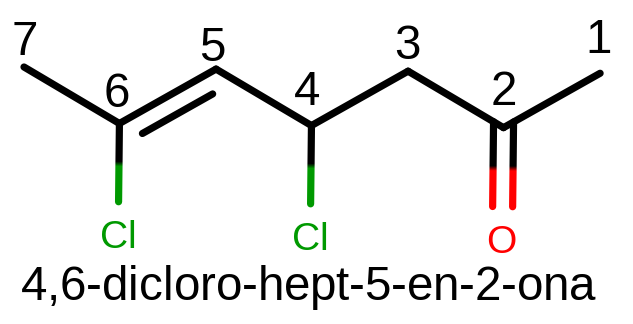
\includegraphics[width=0.45\linewidth]{imagens/46dicloro.png}
\label{fig:46}
\end{figure}

Podemos observar na figura que o hidreto pai consiste em uma cadeia carbônica com 7 átomos, com uma ligação dupla, o que por si só já exige a presença de localizadores, nos obrigando a numerar a cadeia carbônica, restando a dúvida de por onde a iniciar.

A numeração de um hidreto pai (ou um composto pai, mais genericamente), deve ser efetuada por meio da aplicação dos seguinte critérios:

\begin{enumerate}
	\item menor numeração possível para heteroátomos;
	\item menor numeração possível para hidrogênios indicados\footnote{Em determinadas circunstâncias é necessário indicar no nome de um anel, ou sistema de anéis, contendo o número máximo de ligações duplas não cumulativas, uma ou mais posições onde nenhuma ligação múltipla está anexada. Isso é feito especificando a presença de um átomo de hidrogênio 'extra' em tais posições pela citação do local numerado apropriado seguido por um H maiúsculo em itálico};
	
	\begin{figure}[h]
		\centering
		\caption{Exemplos de hidrogênios indicados.}
		\vspace{0.5cm}
		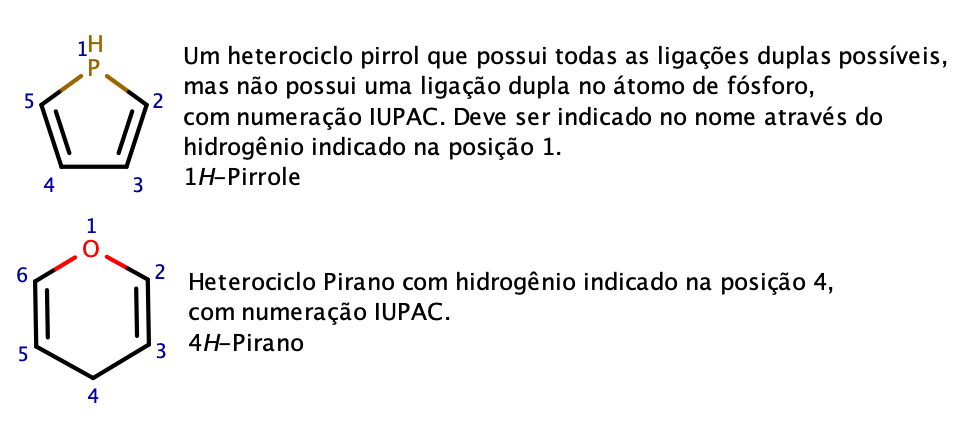
\includegraphics[width=1\linewidth]{imagens/indicado.png}
	\label{fig:indicado}
	\end{figure}

	\item menor posição possível para o grupo funcional principal;
	\item menor posição para insaturações;
	\item menor posição possível para substituintes indicados por prefixos;
	\item menor posição possível para substituintes em ordem de citação.
\end{enumerate}

Nossa próxima dúvida é a seguinte: por qual extremidade da cadeia com 7 átomos de carbono devemos iniciar a numeração? Consultando os dados presentes na tabela \ref{senioridade}, concluímos que o grupo funcional cetona possui maior senioridade (ou prioridade) na numeração, obedecendo o item 3 logo acima. Assim, a numeração do hidreto pai deve se iniciar na extremidade esquerda da cadeia, o que deixa, automaticamente, a ligação dupla na menor posição possível, restando apenas indicar a posição dos dois grupos funcionais (haleto) com menor prioridade, o que explica inequivocamente o nome da substância da figura \ref{fig:46}.

Analise o próximo exemplo, ilustrado na figura \ref{fig:octadieno} a seguir.

\begin{figure}[h]
	\centering
	\caption{Exemplo de aplicação da nomenclatura substitutiva.}
	\vspace{0.5cm}
	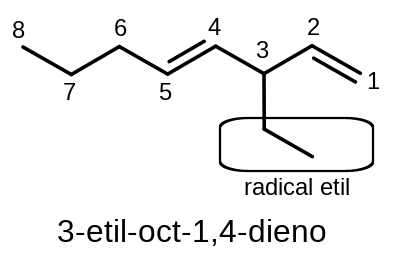
\includegraphics[width=0.6\linewidth]{imagens/octadieno.png}
\label{fig:octadieno}
\end{figure}

Como trata-se de um hidrocarboneto, não há grupos funcionais na disputa por senioridade, deixando a discussão apenas para decisão entre os radicais substituintes e as insaturações. Como estas últimas possuem maior senioridade que os radicais, a numeração da cadeia deve iniciar-se em uma extremidade que deixa as insaturações nas memores posições possíveis da numeração. Finalmente, existe um radical \textbf{etil} conectado ao carbono 3 do hidreto pai. Assim, o nome da substância é \textbf{3-etil-oct-1,4-dieno}. 

Finalizando, convidamos o leitor a examinar a estrutura a seguir, na figura \ref{fig:etenil}, e identificar o número de átomos de carbono do hidreto pai.

\begin{figure}[h]
	\centering
	\caption{Exemplo de aplicação da nomenclatura substitutiva.}
	\vspace{0.5cm}
	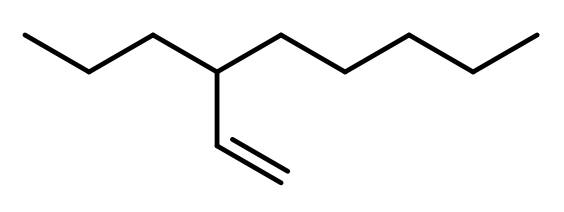
\includegraphics[width=0.6\linewidth]{imagens/etenil.png}
\label{fig:etenil}
\end{figure}

Recomendações da IUPAC anteriores a 2013 sugeriam que o hidreto pai deveria conter eventuais insaturações, mas a recomendação mais atual sugere que o hidreto pai seja aquele com maior número de átomos de carbono, contendo ou não a insaturação. Portanto, o nome da substância da figura \ref{fig:etenil} é mostrado a seguir.

\begin{figure}[h]
	\centering
	\caption{Exemplo de aplicação da nomenclatura substitutiva.}
	\vspace{0.5cm}
	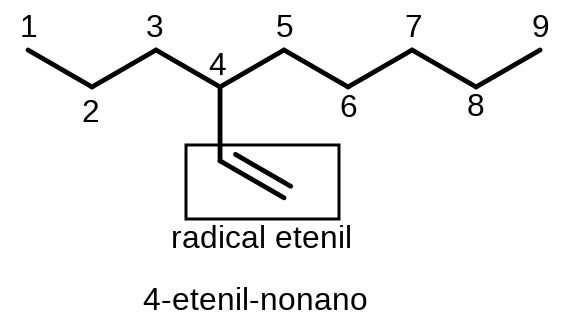
\includegraphics[width=0.6\linewidth]{imagens/nomeetenil.png}
\label{fig:nomeetenil}
\end{figure}

\chapter{Álcoois e fenóis}
\chapter{Álcoois e fenóis}
Iniciando a análise de substâncias orgânicas além de hidrocarbonetos, trataremos aqui sobre álcoois e fenóis, duas funções que apresentam, ao mesmo tempo, semelhanças e diferenças: semelhança pela presença de um grupo OH (hidroxila) e diferença pela presença de um carbono saturado ligado ao grupo OH contra a presença de um carbono aromático ligado ao grupo OH.

Podemos representar, de modo genérico, um álcool pela fórmula geral R-OH, onde R é um radical alquila (metil, etil, isopropil, entre outros) enquanto um fenol é representado pela fórmula geral ArOH, onde Ar é um radical arila (aromático), como fenil, naftil, entre outros.

Álcoois podem ser considerados uma das mais versáteis funções entre aquelas presentes em moléculas orgânicas, pois podem participar de um grande número de reações e formar várias outras funções. Em algumas reações esquematizadas abaixo, a notação \textbf{[O]} indica um reagente oxidamente genérico.

\begin{enumerate}
    \item \textbf{aldeídos}, por meio da oxidação parcial de álcoois primários;
    \begin{figure}[h]
        \centering
        \caption{Oxidação de álcool a aldeído.}
        \vspace{0.5cm}
        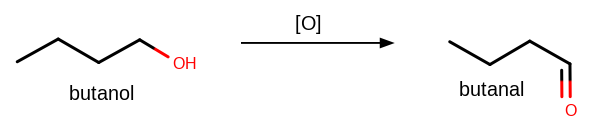
\includegraphics[width=0.75\linewidth]{imagens/alcool-aldeido.png}
    \label{fig:alcoolaldeido}
    \end{figure}

    \item \textbf{cetonas}, por meio da oxidação de álcoois secundários;
    \begin{figure}[h]
        \centering
        \caption{Oxidação de álcool a cetona.}
        \vspace{0.5cm}
        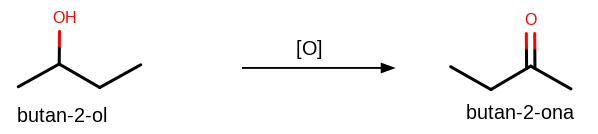
\includegraphics[width=0.75\linewidth]{imagens/alcoolcetona.png}
    \label{fig:alcoolcetona}
    \end{figure}

    \item \textbf{haletos de alquila}, por meio da substituição nucleofílica;
    \begin{figure}[h]
        \centering
        \caption{Substituição nucleofílica de álcoois.}
        \vspace{0.5cm}
        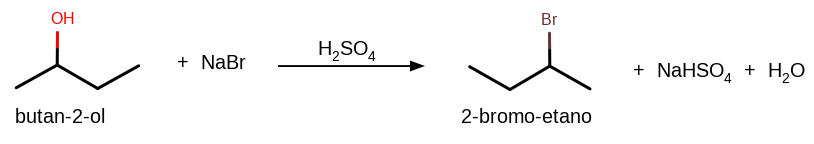
\includegraphics[width=1\linewidth]{imagens/alcoolhaleto.png}
    \label{fig:alcoolhaleto}
    \end{figure}

    \item \textbf{alcenos}, por meio da eliminação intramolecular;
    \begin{figure}[h]
        \centering
        \caption{Desidratação intramolecular de álcoois.}
        \vspace{0.5cm}
        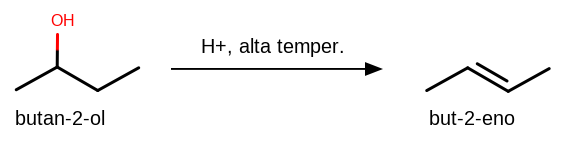
\includegraphics[width=0.85\linewidth]{imagens/alcoolalceno.png}
    \label{fig:alcoolalceno}
    \end{figure}

    \item \textbf{éteres}, por meio da eliminação intermolecular;
    \begin{figure}[h]
        \centering
        \caption{Desidratação intermolecular de álcoois.}
        \vspace{0.5cm}
        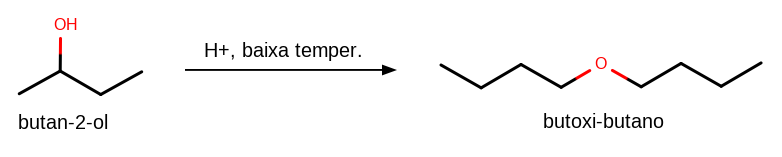
\includegraphics[width=1\linewidth]{imagens/alcooleter.png}
    \label{fig:alcooleter}
    \end{figure}

    \item \textbf{ésteres}, por meio da reação de esterificação;
    \begin{figure}[h]
        \centering
        \caption{Reação de esterificação.}
        \vspace{0.5cm}
        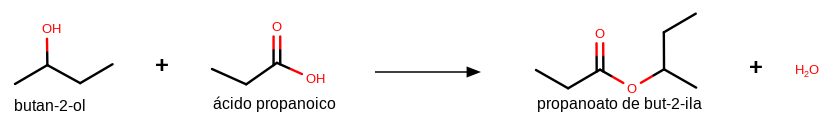
\includegraphics[width=1\linewidth]{imagens/esterificacao.png}
    \label{fig:alcoolester}
    \end{figure}

    \item \textbf{ácidos carboxílicos}, por meio da oxidação completa de álcoois primários\footnote{Embora a oxidação total de um álcool primário seja o processo de descarboxilação oxidativa, usamos aqui o termo "completa" para diferenciar do processo de oxidação parcial de álcoois}. 
    \begin{figure}[h]
        \centering
        \caption{Oxidação total de álcoois primários.}
        \vspace{0.5cm}
        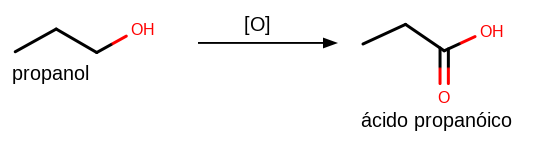
\includegraphics[width=0.85\linewidth]{imagens/alcoolacido.png}
    \label{fig:alcoolacido}
    \end{figure}
\end{enumerate}

\section{Aspectos estruturais}
Em termos estruturais, álcoois e fenóis são, simultaneamente, semelhantes e distintos, pois a presença do grupo OH ligado diretamente a um carbono saturado (álcoois) ou diretamente a um carbono aromático (fenóis) confere propriedades e reatividades distintas às duas funções.

Álcoois apresentam uma característica estrutural muito importante e que ajuda a explicar boa parte de suas propriedades: a possibilidade de formaçào de ligaçòes de hidrogênio com água. A figura \ref{fig:ligacaoh} a seguir ilustra a formação dessa ligação entre etanol (esquerda) e água (direita), explicitada pelo tracejado entre as duas moléculas. Nesta representação, o átomo de carbono é bola de cor cinza, o hidrogênio é a bola branca e o átomo de oxigênio é a bola vermelha.

 \begin{figure}[h]
	\centering
	\caption{Ligação de hidrogênio entre etanol e água, desenhada usando o software Avogadro \cite{avogadro}}
	\vspace{0.5cm}
	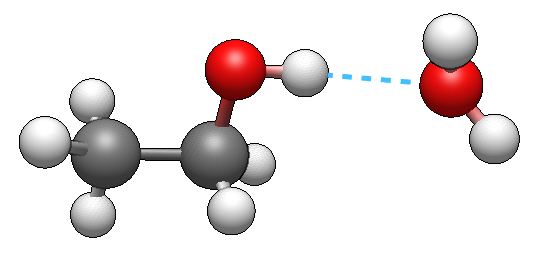
\includegraphics[width=0.85\linewidth]{imagens/ligacaoh.png}
	\label{fig:ligacaoh}
\end{figure}

Isoladamente, as moléculas de propanol e fenol, usadas aqui como exemplo, são analisadas sem a presença de água ou qualquer outro solvente, apenas para ilustrar os efeitos decorrentes da presença do grupo OH nas duas funções. Por uma questão de simplicidade, usaremos apenas a propriedade periódica conhecida como \textbf{eletronegatividade}, juntamente com a \textbf{ressonância}, discutida anteriormente, para explicar as diferenças no caráter ácido/base do propanol e do fenol.

Parte da análise feita nesta seção utiliza o conceito de \textbf{pKa}, uma medida da ionização de uma substância quando encontra-se em solução aquosa.

A definição conceitual de pKa é a constante de equilíbrio de ionização de um ácido fraco. É uma medida da força de um ácido fraco. Quanto menor o pKa, mais forte é o ácido.

Em termos mais simples, o pKa é o pH em que a concentração de ácido não ionizado é igual à concentração de ácido ionizado.

Por exemplo, o ácido acético tem um pKa de 4,76. Isso significa que, em uma solução aquosa com pH de 4,76, a concentração de ácido acético não ionizado é igual à concentração de ácido acético ionizado. Em pHs mais baixos, o ácido acético está mais protonado, ou seja, na forma de ácido. Em pHs mais altos, o ácido acético está mais desprotonado, ou seja, na forma de base.

O átomo de oxigênio do grupo OH, nas duas funções aqui analisadas, encontra-se, inicialmente, com hibridização sp{$^3$} e confere uma relativamente elevada densidade eletrônica na região do grupo OH, conforme por ser observado nas figuras \ref{fig:fenol} e \ref{fig:propanol} a seguir, que ilustram os mapas de potencial eletrostáticos para o fenol e o propanol.

\begin{figure}[h]
    \centering
    \caption{Mapa de potencial eletrostático do fenol}
    \vspace{0.5cm}
    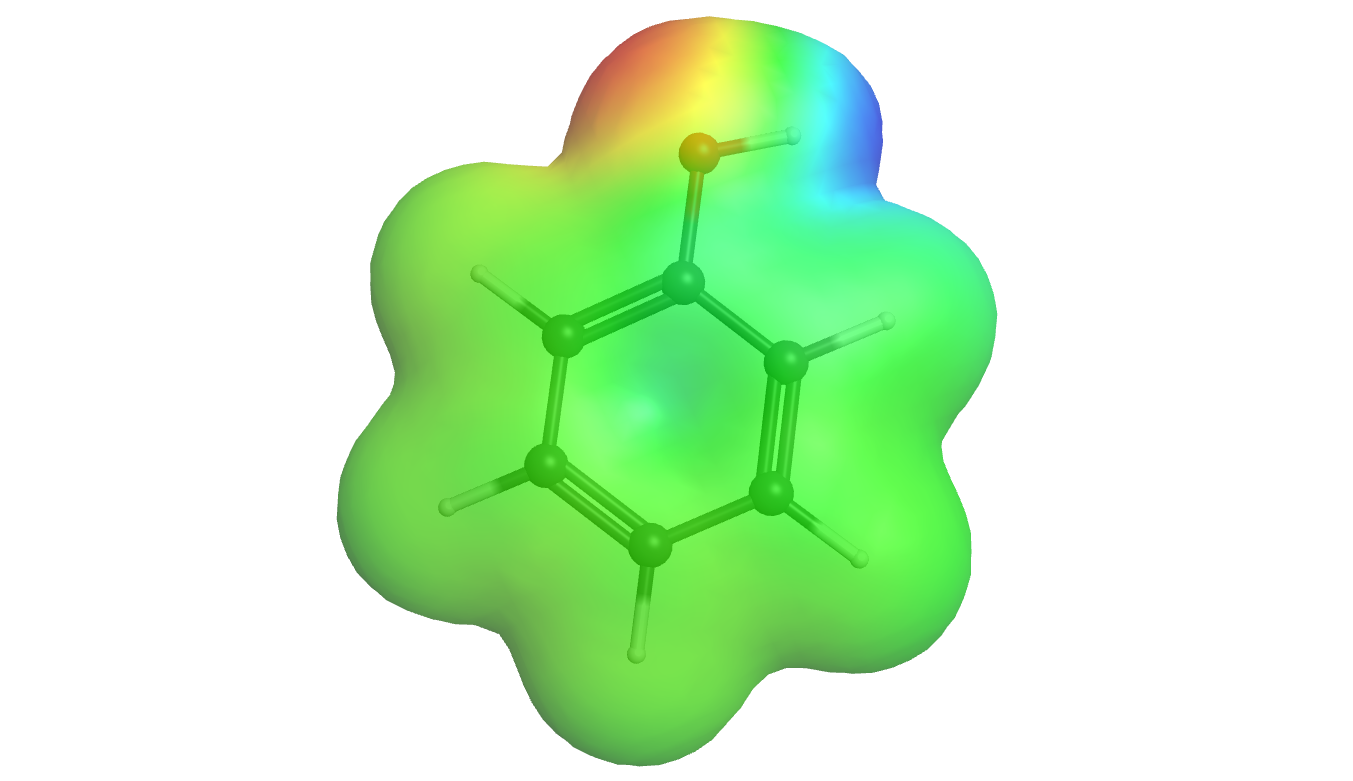
\includegraphics[width=0.6\linewidth]{imagens/fenol.png}
\label{fig:fenol}
\end{figure}

\begin{figure}[h]
    \centering
    \caption{Mapa de potencial eletrostático do propanol}
    \vspace{0.5cm}
    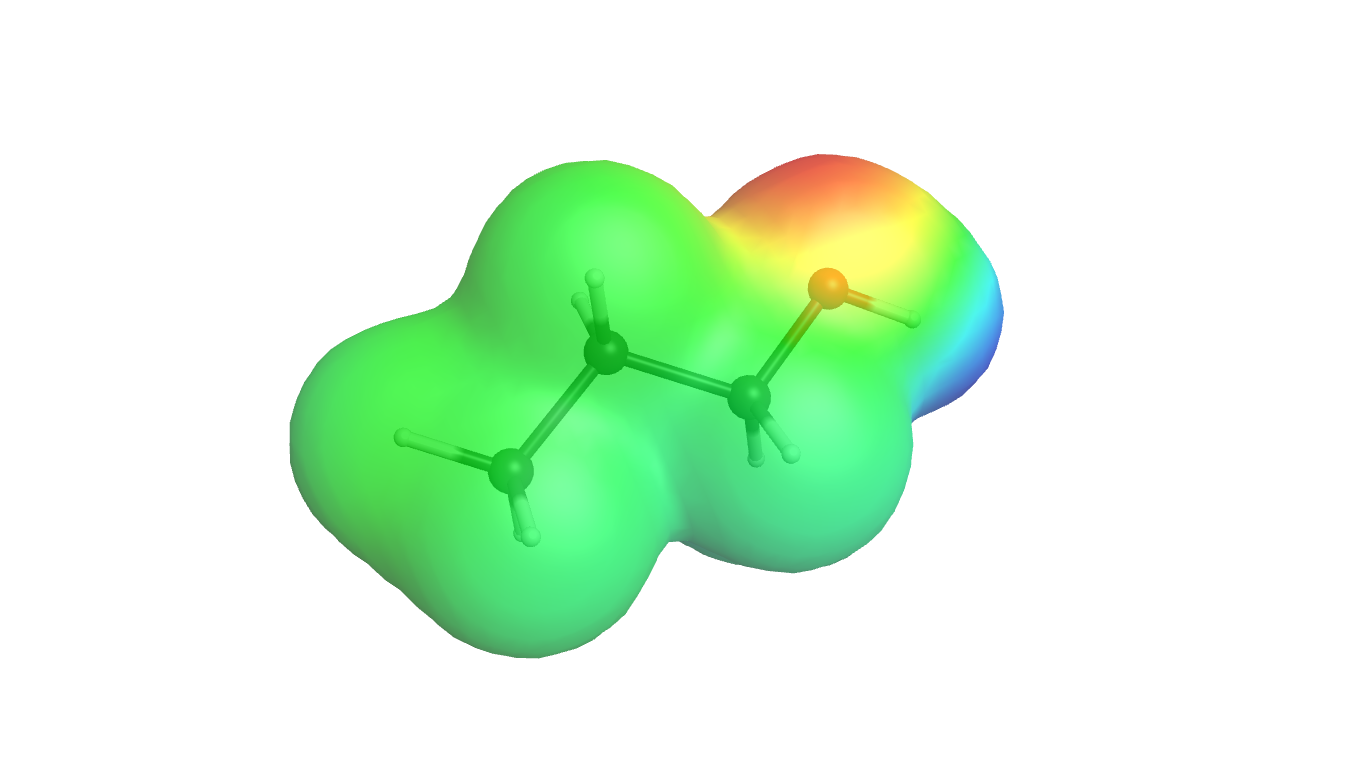
\includegraphics[width=0.75\linewidth]{imagens/propanol.png}
\label{fig:propanol}
\end{figure}

Um ponto interessante a destacar é a existência de estruturas de ressonância associadas ao íon fenolato, obtido pela ionização do fenol em água. Conforma pode ser visto na figura \ref{fig:fenolato} a seguir, a carga eletrônica inicialmente presente no átomo de oxigênio pode ser deslocalizada pelo anel aromático, o que contribui para a estabilização da estrutura como um todo.

\begin{figure}[h]
    \centering
    \caption{Estabilização do fenolato por ressonância}
    \vspace{0.5cm}
    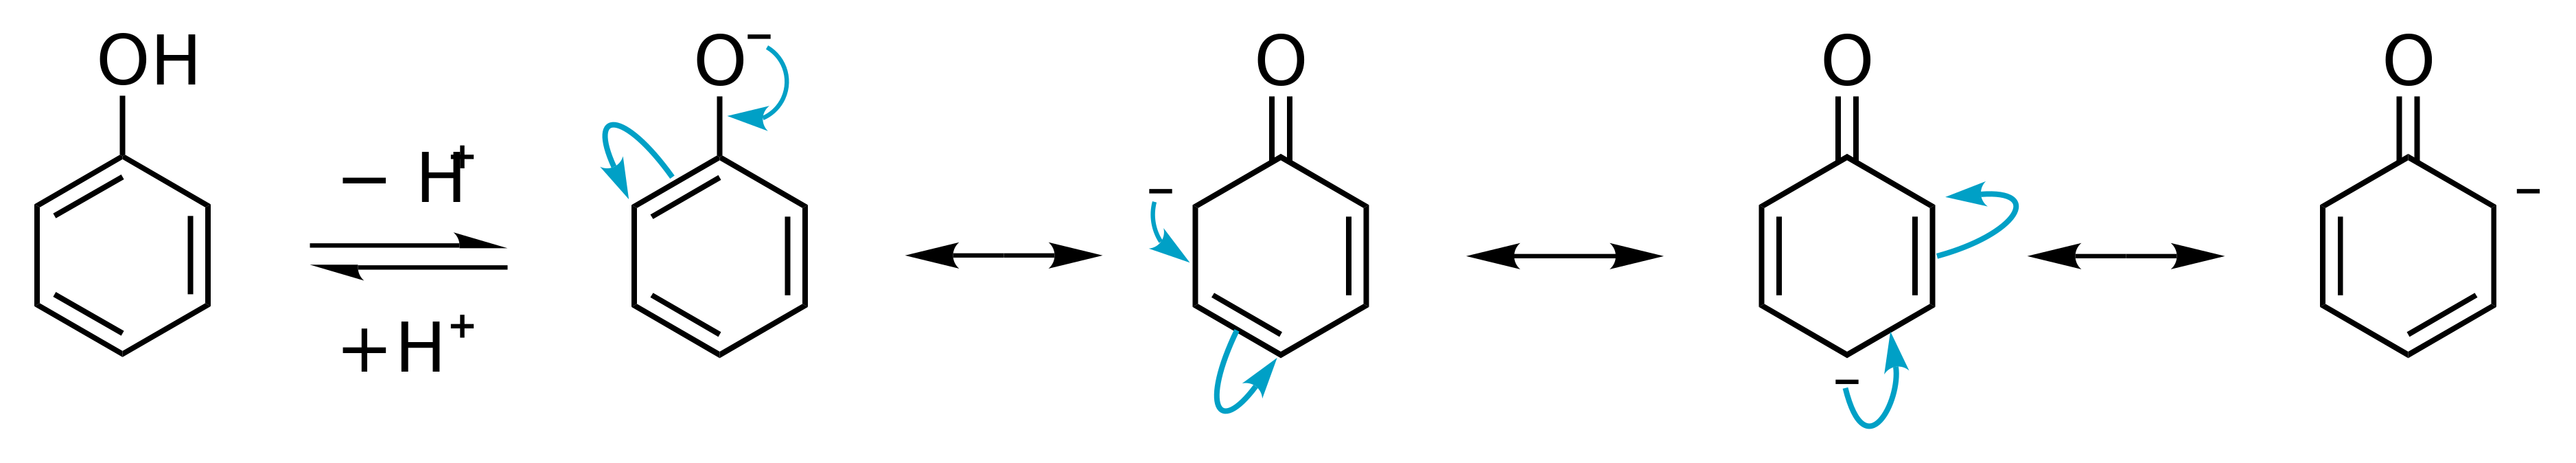
\includegraphics[width=1\linewidth]{imagens/Phenol-phenolate_equilibrium.svg.png}
\label{fig:fenolato}
\end{figure}

As setas indicadas na figura representam a movimentação de elétrons entre as diferentes formas de ressonância possíveis para o íon fenolato, e perceba que a carga negativa resultante da ionização dica deslocalizada pels estrutura.

O mesmo não ocorre no propanol e, portanto, a liberação do cátion H{$^+$} é mais difícil e o fenol apresenta caráter mais ácido que o propanol, uma vez que libera um íon hidrônio com mais facilidade, fato comprovado pelos valores de pKa do fenol (10) e do propanol (16). Uma vez que pKa é uma grandeza expressa em escala logarítmica, um elevado valor de pKa indica um ácido fraco, o que corrobora nossa análise.

Mas por que não ocorre com o propanol? Simples: a força do ácido, considerando o conceito de Brönsted-Lowry, depende da estabilidade da base conjugada, o que deixa o íon hidrônio mais livre. O pronanol não possui um sistema insaturado que permita a estabilização por ressonância.


%################################
\section{Ocorrência e aplicações}
Conforme já mencionado no início deste capítulo, álcoois e fenóis são compostos versáteis e muito úteis em diversos setores econômicos e industriais, e considerando o etanol como um dos protagonistas, por suas aplicações variando de componente de bebidas até combustíveis automotivos, passando por produtos de limpeza, tanto domésticos quanto hospitalares.

\subsection{Álcoois}
Muitos exemplos de substâncias pertencentes à função álcool possuem usos biológicos e/ou aplicações industriais e podemos fixar nossa análise em compostos monofuncionais, ou seja, possuem apenas a função álcool.

\subsubsection{Metanol}
Assim, o mais simples dos álcoois, o composto de fórmula \ce{CH3OH} recebe o nome de metanol, pois possui apenas um carbono e o hidreto pai é o metano. Pela nomenclatura substitutiva, um átomo de Hidrogênio foi substituído pelo grupo OH e álcoois possuem o sufixo ol. Justificado o nome \textbf{metanol}, certo?

\begin{figure}[h]
    \centering
    \caption{Fórmula estrutural para o metanol}
    \vspace{0.5cm}
    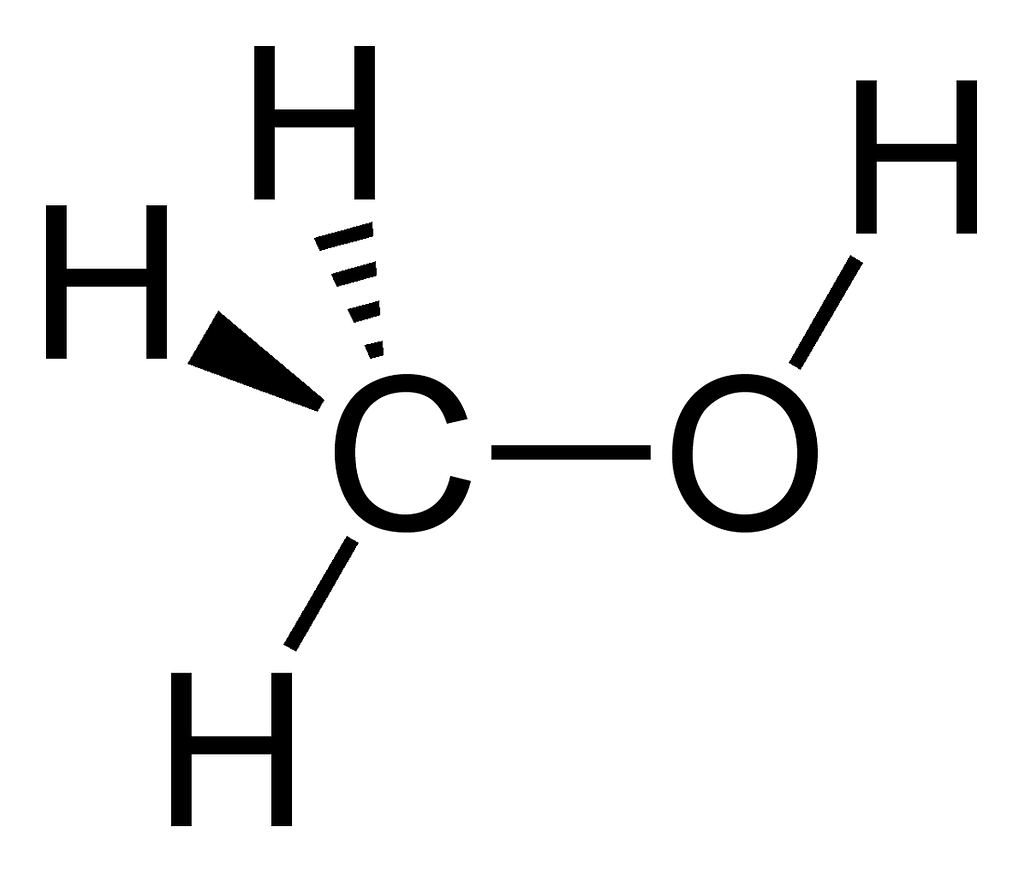
\includegraphics[width=0.35\linewidth]{imagens/methanol-2d-0349e4-1024.png}
\label{fig:mpemetanol}
\end{figure}

A figura \ref{fig:mpemetanol} a seguir ilustra o mapa de potencial eletrostático para o metanol e tal mapa indica a distribuição de cargas elétricas na substância, utilizando uma paleta de cores que vai do azul ao vermelho, onde este último indica maior quantidade de carga em uma dada região, comparada com a cor azul de outra região.

\begin{figure}[h]
    \centering
    \caption{Mapa de potencial eletrostático para o metanol}
    \vspace{0.5cm}
    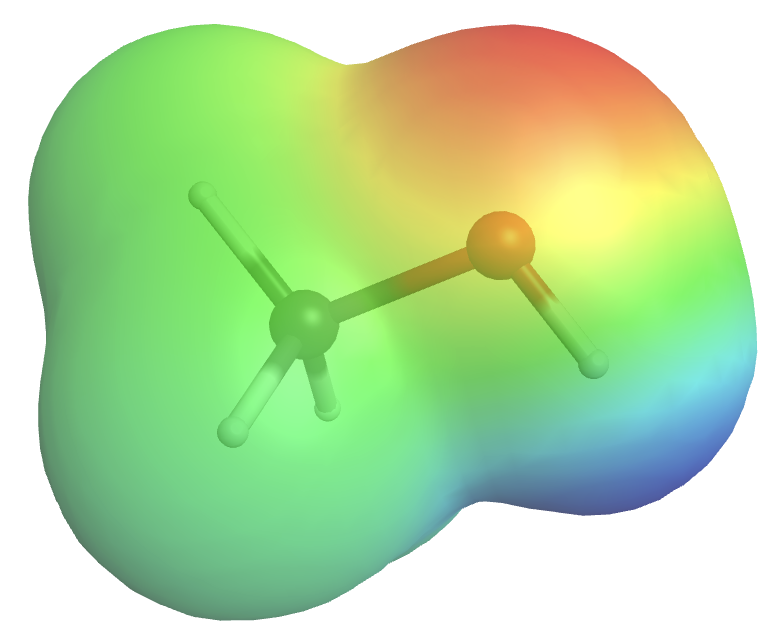
\includegraphics[width=0.45\linewidth]{imagens/mpemetanol.png}
\label{fig:mpemetanol}
\end{figure}

Um estudo recente realizado no Brasil \cite{D2CC01757A} mostra a foto-oxidação de metano para produzir metanol em condições ambientes, catalisada por metais de transição. Comparado com métodos clássicos, as condições reacionais e a possibilidade de uso de luz solar no processo tornam esse estudo muito promissor na produção em escala industrial de metanol.

A toxicidade do metanol, indicada pelo Diagrama de Hommel, indicado na figura \ref{fig:hommel} a seguir, pode ser analisada considerando as quatro partes da imagem contendo números inteiros em uma escala entre 0 e 4, onde 0 indica ausência de problemas e 4 indica perigo crítico.

A figura geométrica do losango é usada pela NFPA (National Fire Protection Association) \footnote{Veja mais em https://www.nfpa.org/codes-and-standards/7/0/4/704}, nos Estados Unidos da América, para indicar riscos associados a cada substância cadastrada na instituição.

A parte em cor vermelha (porção superior do losango) indica a \textbf{inflamabilidade} da substância, ou seja, sua capacidade de entrar em combustão. Portanto, o metanol é bastante inflamável e com um seríssimo agravante: sua combustão gera chamas de cor azul muito claras e visíveis apenas à noite, exigindo mais cuidados em sua manipulação. Diversos acidentes envolvendo metanol já foram citados e aqueles envolvendo automóveis de corrida da chamada Fórmula Indy, categoria automobilística muito famosa nos Estados Unidos da América, são chocantes \footnote{Veja mais em https://www.essentiallysports.com/nascar-news-invisible-fire-at-the-nineteen-eighty-one-indy-five-hundred-sets-the-nascar-community-ablaze-after-fans-make-talladega-superspeedway-nights-connection/}.

A parte em cor azul (porção central e esquerda do losango) indica o \textbf{risco à saúde} e, portanto, o contato ou ingestão deve ser evitado. Para referência, a dose letal por via oral em ratos é de pouco mais de 5,6 g/kg de peso corporal.

A parte em cor amarela (porção central direita do losango) indica \textbf{instabilidade ou reatividade} e mostra a estabilidade do metanol.

A parte em cor branca (porção inferior do losango) indica \textbf{risco específico} (oxidante forte ou radioativo, por exemplo) e não há registros de tal categoria para o metanol.


\begin{figure}[h]
    \centering
    \caption{Diagrama de Hommel para o metanol}
    \vspace{0.5cm}
    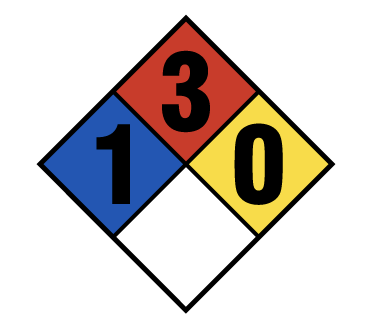
\includegraphics[width=0.25\linewidth]{imagens/hommel.png}
\label{fig:hommel}
\end{figure}

\subsubsection{Etanol}
Este álcool possui tamanha importância no Brasil, seja como combustível, como componente de produtos de limpeza ou em bebidas alcoólicas, que seu nome se confunde com a função orgânica à qual pertence. Por muito tempo os brasileiros compravam "álcool" em postos de combustíveis e apenas recentemente a substância passa a ser comercializada com seu nome oficial.

Trata-se de um líquido transparente, incolor, com densidade em torno de 0,8 g/cm$^3$ e miscível com água em qualquer proporção, explicado por meio da formação de ligações de hidrogênio entre água e etanol de modo tão intenso, que a mistura líquida é classificada como azeótropo, ou seja, os componentes da mistura entram em ebulição juntos, o que inviabiliza a destilação comum como meio de separação dos componentes desta mistura. Porém, é possível separar os componentes da mistura por outros métodos \cite{trica}.

\begin{figure}[h]
	\centering
	\caption{Diferentes representações para o etanol}
	\vspace{0.5cm}
	\includegraphics[width=0.75\linewidth]{imagens/etanol2.jpeg}
	\label{fig:etanol2}
\end{figure}

A figura \ref{fig:etanol2} ilustra ao menos duas representações distintas para o etanol: a fórmula estrutural completa (esquerda) e a representação do tipo "ball \& stick" (tubo e bola) (direita), onde as bolinhas de cores e/ou tamanhos diferentes representam os átomos e os tubinhos representam as ligações químicas entre eles. Existem diferentes representações para moléculas orgânicas em função do contexto de uso, onde uma dada representação pode ser mais esclarecedora que outra.

No Brasil, o etanol é produzido, essencialmente, por fermentação de sacarose por meio de leveduras, em inúmeras usinas de produção espalhadas pelo país, fato que movimenta um enorme número de trabalhadores nos diversos segmentos de produção e distribuição, alimentando uma cadeia produtiva bastante ampla.

Como é produzido a partir da sacarose obtida pela cana-de-açúcar, parte do dióxido de carbono, CO$_2$, produzido pela queima do etanol em motores a combustão, podemos dizer que o etanol é um combustível de ciclo neutro, conforme pode ser visto na figura \ref{fig:neutro} a seguir

 \begin{figure}[h]
 	\centering
 	\caption{Etanol como combustível de ciclo neutro}
 	\vspace{0.5cm}
 	\includegraphics[width=1\linewidth]{imagens/ciclo-neutro.png}
 	\label{fig:neutro}
 \end{figure}

\subsection{Fenóis}
Fenóis são encontrados em muitas fontes vegetais, sendo responsáveis (em parte) pela coloração de flores, frutas e alguns tecidos vegetais, muitas vezes na forma de flavonóides, um tipo de polifenóis bastante comum em plantas, como pode ser visto na figura \ref{fig:taxi} a seguir.

\begin{figure}[h]
    \centering
    \caption{Exemplo de flavonóide: taxifolina.}
    \vspace{0.5cm}
    \includegraphics[width=0.6\linewidth]{imagens/taxifolina.png}
\label{fig:taxi}
\end{figure}

As substâncias pertencentes à função fenol são muito utilizadas biologicamente \cite{doi:10.1021/acs.jmedchem.2c00223}, pois podem apresentar ação:

\begin{itemize}
    \item antioxidante: qualquer substância capaz de impedir ou retardar reações de degradação oxidativa (Figura \ref{fig:toco}), seja por meio da inibição de radicais livres (muito comuns em processos oxidativos) ou então pela formação de complexos metálicos (cátions metálicos formando ligações coordenadas ou dativas com outros íons ou moléculas). 

    \begin{figure}[H]
        \centering
        \caption{Exemplo de fenol com ação anti-oxidante}
        \vspace{0.5cm}
        \includegraphics[width=1\linewidth]{imagens/tocoferol.png}
    \label{fig:toco}
    \end{figure}
    \item antitumoral: O termo "ação antitumoral" refere-se à capacidade de uma substância ou tratamento de inibir ou neutralizar o crescimento e o desenvolvimento de tumores, que são massas anormais de tecido resultantes da divisão celular descontrolada. As ações antitumorais podem ser observadas em vários níveis, visando diferentes aspectos dos processos complexos envolvidos na tumorigênese \footnote{A tumorigênese é o ganho de propriedades malignas em células normais, incluindo principalmente desdiferenciação, proliferação rápida, metástase, evasão da apoptose e imunovigilância, metabolismo desregulado e epigenética, etc., que foram generalizadas como as características do câncer}.
    \begin{figure}[H]
        \centering
        \caption{Exemplo de fenol com ação antitumoral}
        \vspace{0.5cm}
        \includegraphics[width=0.5\linewidth]{imagens/dr.png}
    \label{fig:doxo}
    \end{figure}
    \item antimicrobiana: A ação antimicrobiana refere-se à capacidade de uma substância ou agente de inibir ou matar micro-organismos, como bactérias, vírus, fungos ou protozoários. Esta ação é crucial em vários contextos, incluindo medicina, saúde e preservação de alimentos e outros produtos. Os agentes antimicrobianos podem ser naturais ou sintéticos e são projetados para atingir tipos específicos de microrganismos.
    \begin{figure}[H]
        \centering
        \caption{Exemplo de fenol com ação antimicrobiana}
        \vspace{0.5cm}
        \includegraphics[width=0.65\linewidth]{imagens/triclosan.png}
    \label{fig:triclosan}
    \end{figure}
    \item anti-inflamatória: A ação anti-inflamatória refere-se à capacidade de uma substância ou tratamento de reduzir a inflamação no corpo. A inflamação é uma resposta natural e necessária do sistema imunológico a lesões ou infecção. No entanto, a inflamação crônica ou excessiva pode contribuir para várias condições de saúde, incluindo doenças autoimunes e distúrbios inflamatórios crônicos.

    \begin{figure}[H]
        \centering
        \caption{Exemplo de fenol com ação anti-inflamatória}
        \vspace{0.5cm}
        \includegraphics[width=0.45\linewidth]{imagens/cresotico.png}
    \label{fig:cresotico}
    \end{figure}
    \item anti-hemorrágica: A ação anti-hemorrágica refere-se à capacidade de uma substância ou tratamento de prevenir ou controlar o sangramento. Hemorragia é o termo médico para sangramento excessivo, que pode ocorrer interna ou externamente e pode ser resultado de várias condições ou lesões. Ações anti-hemorrágicas podem ser alcançadas por meio de diferentes mecanismos, e várias substâncias ou intervenções podem exibir essa propriedade \cite{SOUZA2022105299}.
    
    \begin{figure}[H]
        \centering
        \caption{Exemplo de fenol com ação anti-hemorrágica}
        \vspace{0.5cm}
        \includegraphics[width=1\linewidth]{imagens/caju.png}
    \label{fig:caju}
    \end{figure}
\end{itemize}

Porém, nem todos os fenóis apresentam ação biológica benéfica. A substância ácido piridina2,3-dicarboxílico, apresentada na figura \ref{fig:4hexil} apresenta ação neurotóxica, enquanto a outra substância ma mesma imagem apresenta ação antitumoral.

\begin{figure}[ht]
    \centering
    \caption{Exemplos de fenóis com ação biológica}
    \vspace{0.5cm}
    \includegraphics[width=1\linewidth]{imagens/res.png}
\label{fig:4hexil}
\end{figure}

O fenol mais simples conhecido, chamado inicialmente de \textbf{ácido carbólico}, foi utilizado em conjunto (e depois isoladamente) para extermínio em massa de prisioneiros em campos de concentração alemães durante a II Guerra Mundial, por meio de injeção direta no coração dos prisioneiros \cite{triste}.

%#####################
\section{Nomenclatura}
A nomenclatura de compostos monofuncionais da função álcool é bem simples e segue o padrão já visto anteriormente neste texto, considerando a posição do grupo funcional hidroxila para iniciar a numeração da cadeia carbônica. Veja os exemplos a seguir, discutidos caso a caso.

\begin{tcolorbox}[colback=white!5!white,colframe=orange!90!black,title=\textbf{Exemplo 1}]
	\begin{figure}[H]
		\centering
		%\vspace{0.5cm}
		\includegraphics[width=0.3\linewidth]{imagens/isopropanol.png}
		\label{fig:isopropanol}
	\end{figure}
	\tcblower
    A imagem representa um álcool com cadeia carbônica saturada e, portanto, o hidreto pai é chamado de \textbf{propano}. Existe um grupo funcional na posição 2 da cadeia carbônica e, utilizando a nomenclatura substitutiva, a molécula recebe o nome de \textbf{propan-2-ol}, conhecido também pelo nome de \textbf{álcool isopropílico}.
\end{tcolorbox}

\begin{tcolorbox}[colback=white!5!white,colframe=orange!90!black,title=\textbf{Exemplo 2}]
	\begin{figure}[H]
		\centering
		%\vspace{0.5cm}
		\includegraphics[width=0.20\linewidth]{imagens/ciclopentanol.png}
		\label{fig:ciclopentanol}
	\end{figure}
	\tcblower
	A imagem representa um álcool com cadeia carbônica saturada e cíclica com cinco átomos de carbono, e, portanto, o hidreto pai é chamado de \textbf{ciclopentano}. Existe um grupo funcional na posição 1 da cadeia carbônica e, utilizando a nomenclatura substitutiva, a molécula recebe o nome de \textbf{ciclopentan-1-ol}. Em situações como essa, com o único grupo funcional na posição 1, a posição do localizador pode ser omitida..
\end{tcolorbox}


\begin{tcolorbox}[colback=white!5!white,colframe=orange!90!black,title=\textbf{Exemplo 3}]
	\begin{figure}[h]
		\centering
		%\vspace{0.5cm}
		\includegraphics[width=0.20\linewidth]{imagens/cpd.png}
		\label{fig:cpd}
	\end{figure}
	\tcblower
	A imagem representa um álcool com cadeia carbônica insaturada e cíclica com cinco átomos de carbono, fato que exige a posição dos localizadores e implica, naturalmente, na numeração precisa da cadeia carbônica. Como a senioridade do grupo funcional é maior que a da insaturação, a numeração começa no átomo de carbono que sustenta o grupo funcional. Neste caso, a insaturação começa na posição 3 do hidreto pai e, portanto, o nome da substância é \textbf{ciclopent-3-en-1-ol}.
\end{tcolorbox}

\begin{tcolorbox}[colback=white!5!white,colframe=orange!90!black,title=\textbf{Exemplo 4}]
	\begin{figure}[h]
		\centering
		%\vspace{0.5cm}
		\includegraphics[width=0.3\linewidth]{imagens/metilcpd.png}
		\label{fig:metilcpd}
	\end{figure}
	\tcblower
	A imagem representa uma substância muito parecida com a do Exemplo 3, mas com um substituinte que exige a posição de um localizador. Considerando que radicais devem ocupar a menor posição possível, a numeração deve prosseguir, a partir do grupo OH, para a direita e, portanto, o nome da substância é \textbf{2-metil-ciclopent-3-en-1-ol}.
\end{tcolorbox}

\begin{tcolorbox}[colback=white!5!white,colframe=orange!90!black,title=\textbf{Exemplo 5}]
	\begin{figure}[h]
		\centering
		%\vspace{0.5cm}
		\includegraphics[width=0.5\linewidth]{imagens/2metilhex.png}
		\label{fig:2metilhex}
	\end{figure}
	\tcblower
	A imagem representa um álcool com cadeia acíclica, insaturada e com um substituinte. Uma vez que a senioridade do grupo funcional é maior que a da insaturação, a numeração começa na extremidade mais próxima da posição do grupo OH. O próximo passo é indicar a posição dos localizadores e teremos o nome completo da substância: \textbf{2-metil-hex-5-en-3-ol}.
\end{tcolorbox}

\begin{tcolorbox}[colback=white!5!white,colframe=orange!90!black,title=\textbf{Exemplo 6}]
	\begin{figure}[h]
		\centering
		%\vspace{0.5cm}
		\includegraphics[width=0.45\linewidth]{imagens/dmf.png}
		\label{fig:2metilhex}
	\end{figure}
	\tcblower
	O fenol indicado na figura acima possui dois substituintes iguais e sem a presença de localizadores, o que simplifica o nome, permitindo o uso do prefixo \textbf{di} após a numeração da cadeia carbônica. Assim, o nome oficial deste fenole é \textbf{3,5-dimetilfenol}.
\end{tcolorbox}

\begin{tcolorbox}[colback=white!5!white,colframe=orange!90!black,title=\textbf{Exemplo 7}]
	\begin{figure}[h]
		\centering
		\includegraphics[width=0.3\linewidth]{imagens/pcf.png}
		\label{fig:2metilhex}
	\end{figure}
	\tcblower
	O nome deste fenol é um dos mais simples, embora não pareça. O anel benzênico suporta, no máximo, 6 substituintes diferentes e todas as posições nas quais pode haver um substituintes estão ocupadas. Temos cinco substituintes iguais (cloro) e o nome oficial da substância é \textbf{pentaclorofenol}.
\end{tcolorbox}

\begin{tcolorbox}[colback=white!5!white,colframe=orange!90!black,title=\textbf{Exemplo 8}]
	\begin{figure}[h]
		\centering
		%\vspace{0.5cm}
		\includegraphics[width=0.25\linewidth]{imagens/etilmetil.png}
		\label{fig:2metilhex}
	\end{figure}
	\tcblower
	O fenol representado acima apresenta em seu anel aromático dois substituintes diferentes: etil e metil, em posições diferentes. Considerando a regra de manter os localizadores nas menores posições numéricas possíveis, a numeração deve iniciar-se no carbono que sustenta o grupo hidroxila (OH) e então prosseguir para a direita. Substituintes diferentes devem ser citados em ordem alfabética e, assim, o nome oficial deste fenol é \textbf{4-etil-3-metil-fenol}.
\end{tcolorbox}

\begin{tcolorbox}[colback=white!5!white,colframe=orange!90!black,title=\textbf{Exemplo 9}]
	\begin{figure}[ht]
		\centering
		%\vspace{0.5cm}
		\includegraphics[width=0.5\linewidth]{imagens/propofol.png}
		\label{fig:propofol}
	\end{figure}
	\tcblower
	Esta molécula apresenta uma intensa ação anestésica e é conhecida no meio médico com o nome de \textbf{propofol}. Seu PIN (Preferred IUPAC Name) é simples: existem dois radicais iguais nas posições 2 e 6 do anel aromático e devem ser indicados, de acordo com as mais recentes recomendações através do prefixo \textbf{bis}. Mas por que não \textbf{di(propan-2-il)}? Simples: a presença de um localizador (o número 2 dentro dos parênteses) exige o uso dos parênteses e estes exigem o prefixo \textbf{bis}. Portanto, o nome oficial desta molécula é \textbf{2,6-bis-(propan-2-il)fenol}.
\end{tcolorbox}




\chapter{Aldeídos e cetonas}
\chapter{Aldeídos e cetonas}
\begin{mdframed}[backgroundcolor=orange!20,linewidth=0pt,roundcorner=10pt]
	\minitoc
\end{mdframed}
Se você lê este documento, seja em modo impresso ou então em modo digital na tela de um dispositivo qualquer, agradeça a dois aldeídos pela capacidade de leitura. De modo bastante simplificado, a luz refletida de um objeto qualquer incide sobre os fotorreceptores existentes em seus olhos, como bastonetes ou cones, e atinge um aldeído de nome 11-cis-retinal, transformando-o em seu isômero 11-trans-retinal, juntamente com um impulso elétrico que é  interpretado por seu cérebro como um componente de uma imagem.

\begin{figure}[h]
	\centering
	\caption{Isomerização do 11-cis-retinal. A numeração indicada na figura é \textbf{usual} e sem relação com a oficial da IUPAC}
	\vspace{0.5cm}
	\includegraphics[width=0.7\linewidth]{imagens/cistransretinal.png}
	\caption*{Fonte: Autores}
	\label{fig:cistransretinal}
\end{figure}

Os nomes usuais dos aldeídos envolvidos no processo da visão, e mostrados na figura \ref{fig:cistransretinal} apresentam duas partes ainda não analisadas até o momento: \textbf{cis} e \textbf{trans}. São prefixos usados para citar a configuração dos substituintes de uma ligação carbono-carbono do tipo covalente dupla.

A figura \ref{fig:cistrans} ilustra dois isômeros clássicos quando se trata de isomeria cis/trans. Para melhor compreensão dos conceitos, analise a imagem e veja que existe uma linha que trespassa as duas moléculas ao longo da ligação covalente dupla. Esse será nosso eixo de referência.

Na molécula da esquerda, observamos que o átomo de carbono da esquerda da ligação dupla possui dois substituintes distintos: um átomo de Hidrogênio (destacada por um círculo ao seu redor) e um grupo metil (destacada por um quadrado so seu redor). O mesmo ocorre com o átomo de carbono da direita da ligação dupla. Repare que os dois substituintes iguais (ou semelhantes) estão \textbf{do mesmo lado do eixo de referência}: os átomos de Hidrogênio \textbf{acima} e os grupos metil \textbf{abaixo} do eixo. Assim define-se o isômero \textbf{cis}.

Na molécula da direita os grupos iguais ou semelhantes encontram-se \textbf{em lados opostos do eixo de referência} e, desta forma, define-se o isômero \textbf{trans}.		

\begin{figure}[h]
	\centering
	\caption{Exemplo de uso dos prefixos cis e trans na nomenclatura em Química Orgânica}
	\vspace{0.5cm}
	\includegraphics[width=0.85\linewidth]{imagens/cistrans.png}
	\caption*{Fonte: Autores}
	\label{fig:cistrans}
\end{figure}

Aldeídos e cetonas são duas funções orgânicas que apresentam o chamado grupo \textbf{carbonil} (C=O), o que as torna duas das mais versáteis funções da Química Orgânica. Você já ficou curioso a respeito da origem do nome da função orgânica aldeído? Espero que sim. O nome \textbf{aldeído} tem origem na expressão (em inglês) \textbf{al}cohol \textbf{dehyd}ration, comprovado pela transformação do etanol em etanal, realizada no fígado e catalisada pela enzima \textbf{álcool desidrogenase}.

O grupo carbonil é muito versátil por participar de inúmeras reações e várias delas serão discutidas nesta obra. Cabe gora uma análise estrutural do grupo carbonil, usando o mais simples dos aldeídos como exemplo.

\begin{figure}[h]
	\centering
	\caption{Estrutura do metanal}
	\vspace{0.5cm}
	\includegraphics[width=0.35\linewidth]{imagens/formaldeido2.png}
	\caption*{Fonte: Autores}
	\label{fig:}
\end{figure}

O grupo carbonil é formado por um átomo de carbono unido a um átomo de oxigênio por uma ligação covalentes dupla, e também a dois átomos de hidrogênio por uma ligação covalente simples. 
O átomo de carbono do grupo carbono possui hibridização sp$^2$, o que confere ao grupo uma geometria plana na forma de um triângulo e agrupando as duas informações nós temos a chamada geometria \textbf{trigonal plana}, onde o ângulo diedro entre o carbono e os dois átomos de hidrogênio é de 120°. 
A planaridade do grupo carbonil permite a ocorrência de reações de adição que podem ocorrer na superfície superior ou na superfície inferior do grupo carbono, formando produtos com arranjos espaciais distintos, bastante versátil quando utilizado em reações de síntese orgânica, e, ao mesmo tempo, forma em alguns casos mistura de produtos de difícil separação.
A diferença de eletronegatividade entre o carbono e o oxigênio faz com que a ligação covalentes dupla seja polarizada e o lado negativo está mais próximo do átomo de oxigênio. Esta característica estrutural justifica a existência de híbridos de ressonância conforme pode ser visto na figura \ref{fig:hibridos} ao longo deste texto.

Usando um aldeído simples como exemplo, podemos verificar, na figura \ref{fig:etanal}, que existe uma região no grupo carbonila onde a densidade eletrônica é mais elevada, o que indica duas situações complementares entre si: 

\begin{itemize}
	\item \textbf{elevada polarização} da ligação C=O
	\item \textbf{alta reatividade} como consequência da polarização.
\end{itemize}

\begin{figure}[h]
	\centering
	\caption{Mapa de densidade eletrônica para o etanal.}
	\vspace{0.5cm}
	\includegraphics[width=0.5\linewidth]{imagens/etanal.png}
	\caption*{Fonte: Autores}
	\label{fig:etanal}
\end{figure}

A origem da região com elevada densidade eletrônica pode ser explicada por meio da eletronegatividade \footnote{tendência de um átomo em atrair para si os elétrons de uma ligação covalente} ou então por meio da polarizabilidade \footnote{tendência de um átomo ou molécula em ter seus elétrons deslocados por meio de um campo elétrico externo}. A diferença de eletronegatividade entre os átomos de Carbono e Oxigênio no grupo carbonila permite a existência de híbridos de ressonância, conforme mostrado na figura \ref{fig:hibridos}. Tal estrutura está envolvida nas reações orgânicas das quais os aldeídos e as cetonas participam, e que serão analisadas em outro ponto desta obra. A região com mais elevada densidade eletrônica encontra-se na parte superior esquerda da figura.

\section{Propriedades físicas}
Na ausência do híbrido de ressonância (uma vez que tais estruturas ocorrem em condições e ambientes reacionais), conforme pode ser visto na figura \ref{fig:hibridos}, com cargas elétricas positivas e negativas plenas, as moléculas de aldeídos e cetonas apresentam-se bastante polarizadas, trazendo consequências nos valores das propriedades físicas mais comuns, como Ponto de Fusão (PF), Ponto de Ebulição (PE) e Pressão de Vapor (PV). De modo geral, aldeídos e cetonas apresentam valores de PF e PE maiores que hidrocarbonetos de mesma massa molar, uma vez que suas moléculas atraem-se por meio de interações mais fortes que aquelas presentes em hidrocarbonetos. Veja a tabela \ref{pfalcanos} para alguns valores que comprovam nossa breve análise.

\vspace{0.5cm}
\begin{table}[!h]
	%\begin{tabular}
	\begin{center}
	\caption{\label{pfalcanos}Comparativo de propriedades físicas (PE, em $^o$C) de hidrocarbonetos, aldeídos e cetonas (a menos cetona possível possui 3 carbonos em sua estrutura).}
	\vspace{0.5cm}
	\begin{tabular}{c c c c}
	\hline
	Num. carbonos & Alcano & Aldeído & Cetona\\
	\hline
	1 & -162 & -19,5 & -- \\
	2 & -89 & 20,2 & -- \\
	3 & -42 & 48.8 & 56,2 \\
	4 & 0 & 74,8 & 79,6 \\
	5 & 36 & 100,3 & 101 \\
	\hline
	\end{tabular}
	\end{center}
	\caption*{Fonte: Autores}
\end{table}

\begin{figure}[h]
	\centering
	\caption{Híbridos de ressonância no etanal}
	\vspace{0.5cm}
	\includegraphics[width=0.85\linewidth]{imagens/hibridos.png}
	\caption*{Fonte: Autores}
	\label{fig:hibridos}
\end{figure}

A polaridade de uma molécula (polar ou apolar) pode ser determinada, de modo muito simples, ao dissolve-la em um solvente polar ou apolar. Sabendo que moléculas polares dissolvem-se em solventes polares e que ocorre o mesmo para moléculas apolares, um teste químico em laboratório pode concluir se a molécula é polar ou não.

Porém, pode ser necessário saber o quão polar ou apolar é essa molécula, e esta tarefa pode ser feita com ajuda de um software aplicado à Química Orgânica, como por exemplo \cite{avogadro}, utilizado na construção de algumas imagens nesta obra. A figura \ref{fig:polaridade} mostra o resultado do cálculo da polaridade do etanal. 

\begin{figure}[h]
	\centering
	\caption{Polaridade calculada do etanal}
	\vspace{0.5cm}
	\includegraphics[width=0.75\linewidth]{imagens/polaridadeetanal}
	\caption*{Fonte: Autores}
	\label{fig:polaridade}
\end{figure}

Embora pareça desproporcional, a seta à direita da imagem \ref{fig:polaridade} é desenhada pelo software após o cálculo do momento dipolar do etanal \cite{raymond2015chemistry}. O calor calculado é de \textbf{2,472 D} (Debye). Apenas como referência, a água é conhecida por ser um solvente polar, apresenta momento dipolar de \textbf{1,855 D}, mostrando que o etanal é bem mais polar que a água, ou seja, apresenta assimetria na distribuição de cargas elétricas muito maior que na água \footnote{Momento dipolar é uma grandeza vetorial que representa a polaridade de um sistema de cargas elétricas. É definido como o produto da carga elétrica pela distância entre as cargas, e tem a direção do segmento de reta que une os centros das cargas, apontando ao lado maior densidade eletrônica.}.

Essa polaridade elevada faz com que o etanal seja solúvel em água para quaisquer proporções, assim como o etanol, e uma simulação realizada com o software Avogadro \cite{avogadro} mostrou a formação de uma ligação de Hidrogênio entre o átomo de Oxigênio do grupo carbonil e um dos átomos de Hidrogênio da água. Uma imagem dessa simulação pode ser vista na figura \ref{fig:etanalagua}, onde o tracejado representa a ligação de Hidrogênio. Na figura, por uma característica do software, os átomos de Hidrogênio são as bolinhas claras e menores, os átomos de Carbono são as bolinhas maiores e mais escuras, enquanto os átomos de Oxigênio são as bolinhas de tamanho intermediário e de cor vermelha.

Naturalmente, estas ligações de Hidrogênio não ocorrem apenas com um dos átomos de Hidrogênio da água, mas sim \textbf{todos} os átomos de Hidrogênio da água e com os dois pares eletrônicos não compartilhados do átomo de Oxigênio, formando uma espécie rede intermolecular, parecida com a que ocorre entre moléculas de água. Tal fato ajuda a explicar a elevada solubilidade do etanal em água.
 
\begin{figure}[H]
	\centering
	\vspace{0.25cm}
	\caption{Formação de ligação de hidrogênio entre etanal e água.}
	\vspace{0.25cm}
	\includegraphics[width=0.85\linewidth]{imagens/etanal_agua.png}
	\caption*{Fonte: Autores}
	\label{fig:etanalagua}
\end{figure}

E os demais aldeídos? Apresentam o mesmo comportamento? Não, não apresentam. Aldeídos com cadeias carbônicas maiores sofrem mais a influência da baixa polaridade da porção hidrocarboneto, comparada com o grupo carbonil, e são menos solúveis em água.

Cetonas apresentam o mesmo comportamento dos aldeídos quando se trata de solubilidade em água, e cetonas com moléculas pequenas são bem solúveis em água, e, à medida em que as cadeias carbônicas aumentam de tamanho, ajudam a quebrar as eventuais ligações de Hidrogênio entre aldeídos ou cetonas e água. Isso explica a diminuição da solubilidade, em água, de aldeídos e cetonas com cadeias carbônicas maiores.

\section{Nomenclatura}
A nomenclatura de aldeídos e cetonas está diretamente relacionada com a presença do grupo carbonil, e apresentam diferentes sufixos:
 \begin{itemize}
	\item \textbf{aldeídos}: al
	\item \textbf{cetonas}: ona
 \end{itemize}

 \subsection{Aldeídos}
A principal característica estrutural de aldeídos é o grupo funcional localizar-se sempre na extremidade do hidreto pai. Com isso, a numeração da cadeia para identificação precisa dos localizadores inicia-se sempre na posição do grupo funcional.

\begin{figure}[h]
	\centering
	\vspace{0.25cm}
	\caption{Exemplo de nomenclatura de aldeído acíclico.}
	\vspace{0.25cm}
	\includegraphics[width=0.45\linewidth]{imagens/butanal.png}
	\caption*{Fonte: Autores}
	\label{fig:butanal}
\end{figure}

A composição do nome do aldeído é realizada utilizando-se a nomenclatura substitutiva, onde o sufixo \textbf{o} do hidreto pai é substituído pelo sufixo \textbf{al} dos aldeídos. Um hidrocarboneto com quatro carbonos chama-se \textbf{butano} e, portanto, o aldeído com mesmo número de átomos de carbono, exibido na figura \ref{fig:butanal}, chama-se \textbf{butanal}.

Quando o aldeído é substituído, ou seja, um ou mais átomos de Hidrogênio foram substituídos por outros átomos ou grupos de átomos, todos os substituintes precisam ter seu nome e localização na cadeia carbônica, seguindo a ordem alfabética dos nomes dos substitutintes, conforme pode ser visto na figura \ref{fig:aldeidosubst}.

\begin{figure}[H]
	\centering
	\vspace{0.25cm}
	\caption{Exemplo de nomenclatura de aldeído acíclico e substituído.}
	\vspace{0.25cm}
	\includegraphics[width=0.45\linewidth]{imagens/aldeidosubst.png}
	\caption*{Fonte: Autores}
	\label{fig:aldeidosubst}
\end{figure}

O aldeído ilustrado na figura \ref{fig:aldeidosubst} apresenta três substituintes e, portanto, precisamos definir três localizadores. Considerando os nomes dos substitutintes (metil, cloro e hidroxi), a ordem alfabética destes é \textbf{cloro}, \textbf{hidroxi} e \textbf{metil}. Para compor o nome do aldeído, cite os nomes dos substituintes em ordem alfabética, mas explicitando os respectivos localizadores (3, 4 e 2). Assim, o nome do aldeído é \textbf{3-cloro-4-hidroxi-2-metil-pentanal}.

O cenário muda ligeiramente quando o hidreto pai do aldeído apresenta cadeia cíclica. Nestes casos, o sufixo do aldeído passa a ser \textbf{carbaldeído} e o átomo de Carbono que sustenta o grupo funcional é numerado como 1, com ao menos uma exceção, discutida a seguir, relacionada ao hidrocarboneto chamado \textbf{naftaleno}, ilustrado na figura \ref{fig:naftaleno}.

\begin{figure}[h]
	\centering
	\vspace{0.5cm}
	\caption{Naftaleno}
	%\vspace{0.25cm}
	\includegraphics[width=0.25\linewidth]{imagens/naftaleno.png}
	\caption*{Fonte: Autores}
	\label{fig:naftaleno}
\end{figure}

Esta molécula é bastante simétrica e, portanto, não existem tantas posições distintas na cadeia cíclica como se pode perceber ao analisar a imagem rapidamente. Precisamos lembrar, neste momento, de um conceito simples: \textbf{plano de simetria}. Esta entidade pode ser compreendida como um corte que pode ser feito em, por exemplo, algum objeto e que o divide em duas metades idênticas. 

A molécula do naftaleno admite \textbf{dois planos de simetria}, um deles ao longo da ligaçào covalente comum aos dois ciclos e outro perpendicular a esse primeiro, que dividem a molécula em \textbf{quatro partes idênticas}. Considere qua o naftaleno possui fórmula molecular \ce{C10H8} e estes 8 átomos de Hidrogênio serão igualmente divididos em cada uma dessas quatro partes idênticas. Assim, temos apenas \textbf{dois átomos de Hidrogênio distintos} e não 8 como se percebe sem analisar os conceitos de simetria.

A análise cuidadosa da imagem \ref{fig:simetria} mostra os três planos de simetria presentes na molécula de naftaleno (incluindo aquele que trespassa os átomos ao meio), dividindo-a em quatro quadrantes idênticos, cada um deles contendo dois átomos de Carbono e dois átomos de Hidrogênio. Repare que todos os átomos de carbono estão todos no mesmo plano na posição central da imagem e identificados por meio de bolinhas escuras, conectadas entre si.

\begin{figure}[h]
	\centering
	\vspace{0.5cm}
	\caption{Elementos de simetria presentes no naftaleno}
	%\vspace{0.25cm}
	\includegraphics[width=0.5\linewidth]{imagens/simetria.png}
	\caption*{Fonte: Verifique nas referências}
	\label{fig:simetria}
\end{figure}

Uma outra imagem pode deixar o conceito todo ainda mais claro \cite{sym13040526}, como pode ser observado na figura \ref{fig:simetria2}.

\begin{figure}[h]
	\centering
	\vspace{0.5cm}
	\caption{Simplificação dos elementos de simetria presentes no naftaleno}
	%\vspace{0.25cm}
	\includegraphics[width=0.35\linewidth]{imagens/simetria3.png}
	\caption*{Fonte: Autores}
	\label{fig:simetria2}
\end{figure}

Na figura \ref{fig:simetria2}, podemos perceber que a combinação das duas setas divide a molécula do naftaleno em quatro quadrantes \textbf{idênticos}, identificados pelas letras A, B, C e D. Atente-se ao fato de que os quadrantes A e B são \textbf{imagens especulares} um do outro e que ocorre o mesmo entre os quadrantes C e D. Ainda, os quadrantes A e C também são imagens especulares um do outro, assim como os quadrantes B e D. Os dois átomos de Carbono e os dois átomos de Hidrogênio em cada quadrante são diferentes entre si, o que justifica a numeração oficial do naftaleno, vista na figura \ref{fig:numerado}. Tecnicamente, um \textbf{eixo de simetria} é diferente de um \textbf{plano de simetria}, mas a simetria do naftaleno não mudou com a representação simplificada, e o uso das setas pode deixar o tópico mais claro para alguns leitores.

\begin{figure}[h]
	\centering
	\vspace{0.5cm}
	\caption{Numeração oficial do naftaleno}
	%\vspace{0.25cm}
	\includegraphics[width=0.35\linewidth]{imagens/numerado.png}
	\caption*{Fonte: Autores}
	\label{fig:numerado}
\end{figure}

Compreendida a numeração da cadeia carbônica do naftaleno, podemos analisar a segunda parte de nossa exceção, para que o nome de um aldeído visto pouco adiante fique plenamente esclarecida.

Repare que a molécula do naftaleno (figura \ref{fig:naftaleno}) apresenta cinco ligações covalentes duplas e, para "desaromatizar" o naftaleno por um processo chamado de \textbf{hidrogenação} (reação orgânica que consiste na adição de moléculas de H$_2$ a cadeias insaturadas, na proporção de \textbf{1 molécula de H$_2$ para cada ligação dupla}), são necessárias 5 moléculas de H$_2$ ou 10 átomos de Hidrogênio, conforme pode ser visto na figura \ref{fig:hidrogenacao}. Não foram citadas na reação a presença de qualquer catalisador e tampouco condições de temperatura e pressão, uma vez que trata-se de um esquema simplificado. Em tempo: a molécula formada através da hidrogenação do naftaleno (deca-hidronaftaleno) mantém a mesma numeração do naftaleno.

\begin{figure}[h]
	\centering
	\vspace{0.5cm}
	\caption{Reação de hidrogenação do naftaleno}
	%\vspace{0.25cm}
	\includegraphics[width=1\linewidth]{imagens/hidrogenacao.png}
	\caption*{Fonte: Autores}
	\label{fig:hidrogenacao}
\end{figure}

Podemos analisar agora um conjunto de moléculas da função aldeído, visto na figura \ref{fig:conjunto}, inicialmente identificados pelas letras A, B, C e D, onde praticaremos as regras de nomenclatura de aldeídos, herdando as regras gerais da IUPAC. Lembre-se que é necessário identificar o hidreto pai, bém os localizadores, pois cada substituinte exige seu localizador correspondente e, no caso de mais de um substituinte, considere sempre ordem alfabética ao citar os mesmos.

\begin{figure}[H]
	\centering
	\vspace{0.5cm}
	\caption{Exemplos de nomes de aldeídos diversos}
	%\vspace{0.25cm}
	\includegraphics[width=0.65\linewidth]{imagens/exemplosaldeidos.png}
	\caption*{Fonte: Autores}
	\label{fig:conjunto}
\end{figure}

\begin{description}
	\item[\textbf{Substância A}]: trata-se de um aldeído no qual o hidreto pai é uma cadeia cíclica e, portanto, o grupo carbonil passa a chamar-se \textbf{carbaldeído} e ligado à posição do anel ciclopentânico. Assim, o nome da substância é \textbf{ciclopentanocarbaldeído}. 
	\item[\textbf{Substância B}]: o hidreto pai deste aldeído é o hidrocarboneto chamado ciclo-hexano e o grupo carbonil está ligado ao carbono numerado como 1 na cadeia do hidreto pai. Existem ainda dois substitutintes chamados \textbf{metil} com os localizadores 2 e 4. Assim, este aldeído é chamado de \textbf{2,4-dimetil-ciclo-hexanocarbaldeído}. 
	\item[\textbf{Substância C}]: este aldeído é derivado do naftaleno por meio da reação de hidrogenação total. Repare que o hidreto pai, conforme visto anteriormente, chama-se \textbf{deca-hidronaftaleno}, porque a reação de hidrogenação inseriu 10 novos hidrogênios, o que justifica o prefixo \textbf{deca}. O grupo funcional encontra-se na posição 2 do hidreto pai, conforme discutido anteriormente. Portanto, o nome do aldeído aqui analisado é \textbf{deca-hidronafataleno-2-carbaldeído}.  
	\item[\textbf{Substância D}]: o nome desta substância é mais simples que os demais, uma vez que o substituinte formado por um átomo de Carbono ligado ao anel aromático é chamado de \textbf{benzil}, considerado legado pela IUPAC. Portanto, o nome deste aldeído é \textbf{benzaldeído}.
\end{description}

 \subsection{Cetonas}
 
 \begin{minipage}{\textwidth} 
 	\begin{figure}[H]
 		\caption{\label{fig:label} Figure title}
 		\includegraphics[width=0.25\linewidth]{imagens/cpd.png}
 	\end{figure}
 \end{minipage}


%\chapter{Aldeídos e cetonas}
%\chapter{Ácidos carboxílicos e derivados}
%\chapter{Haletos orgânicos}
%\chapter{Compostos nitrogenados}
%\chapter{Compostos sulfurados}
%\chapter{Bioquímica}
\part{Nomenclatura Geral em Química Orgânica}
\section{Nomenclatura de hidrocarbonetos}
Assim como qualquer outra substância, todo hidrocarboneto precisa de ao menos dois conjuntos de informação: (a) uma fórmula que caracteriza suas propriedades e (b) um nome que define sua unicidade. Uma vez que são conhecidos centenas de milhares de hidrocarbonetos distintos, torna-se obrigatório o uso de alguma sistematização para criação de nomes únicos.

Esta imensa tarefa está centralizada na entidade conhecida como IUPAC (International Union for Pure and Applied Chemistry, ou União Internacional para Química Pura e Aplicada) e está registrada no chamado "BlueBook", documento específico para nomenclatura de substâncias orgânicas.

Devemos alertar o leitor que, uma vez que são conhecidas milhões de substâncias orgânicas, a quantidade de regras e orientações sugeridas pela IUPAC é relativamente grande e abordaremos neste documento, aos poucos, parte dessas regras, pois nossa obra tem escopo bem definido não necessita de todas as regras. Deixamos aqui a curiosidade do leitor na leitura das regras previstas na versão 3 do BlueBook.

São necessários alguns conceitos introdutórios antes de aplicarmos as regras de nomenclatura em Química Orgânica:

\subsection{Cadeia carbônica principal}
Substâncias orgânicas normalmente possuem vários átomos de carbono e em todas elas existe uma \textbf{sequência única de átomos de carbono que é a maior possível}. Esta é a \emph{cadeia principal}. Eventuais átomos ou grupos de átomos que não fazem parte da cadeia principal são chamados de \textbf{radicais}. A figura \ref{fig:23} a seguir ilustra os conceitos necessários para iniciar a compreensão do processo de identificação e numeração da cadeia carbônica principal.

\begin{figure}[H]
	\centering
	\caption{Cadeia carbônica principal e radicais}
	\vspace{0.5cm}
	\includegraphics[width=0.75\linewidth]{imagens/23dimetil-hexano.png}
	\label{fig:23}
\end{figure}

Repare que a representação molecular acima é chamada de "bastão" e tem algumas peculiaridades. Nesta representação, as ligações entre átomos de carbono são exibidas como traços (um, dois ou três traços para representar ligações simples, duplas e triplas, respectivamente), em função do caráter covalente dessas ligações, e as ligações entre átomos de carbono e átomos de hidrogênio são \textbf{omitidas} para clareza da representação. As demais ligações precisam ser exibidas.

A cadeia carbônica principal é a maior sequência única de carbonos na molécula, identificada pela sequência numérica de 1 a 6, conforme ilustrado na figura \ref{fig:23} exibida acima. Repare que dois átomos de carbono não fazem parte da cadeia principal e, portanto, são considerados \textbf{radicais}, assim como quaisquer conjuntos de átomos fora da cadeia principal. A nomenclatura de radicais será vista um pouco mais adiante.

\subsection{Radicais}
	
Embora não façam parte da cadeia principal, os radicais fazem parte da molécula e, deste modo, são descritos no nome da molécula. Na figura \ref{fig:23}, temos dois radicais: um deles conectado ao carbono 2 da cadeia principal e outro conectado ao carbono 3. Cada um destes radicais é formado por um átomo de carbono e três átomos de hidrogênio (para completar a tetravalência do carbono), e representados por \textbf{\ce{CH3}}. Este radical chama-se \textbf{metil} e razão deste nome é bem simples: espécies que possuem apenas um átomo de carbono recebem o prefixo \textbf{met}. Além disso, todo radical possui sufixo \textbf{il}.

Muitos dos nomes que você encontrará em livros, apostilas e provas mundo afora são considerados triviais pela IUPAC e os nomes oficiais são, mais uma vez, inequívocos para que você entenda e aplique uma regra sem depender apenas de memória. Veja alguns exemplos:

\textbf{\ce{CH3.}} : esta é a representação sugerida pela IUPAC para o radical metil, uma vez que houve, hipoteticamente, uma quebra homolítica de uma ligação covalente entre carbono e hidrogênio para que se forma o radical citado. Porém, por razões de simplificação didática, o mesmo radical é representado como \ce{CH3-}.

Para deixar ainda mais claro que nomes tradicionais ainda são MUITO utilizados na nomenclatura de substâncias orgânicas, a figura \ref{fig:isopropil} ilustra a estruturas do radical comum em várias substâncias orgânicas e chamado de isopropil (nome tradicional). De acordo com as regras oficiais da IUPAC, o nome oficial do radical é \textbf{propan-2-il}, indicando um conjunto com 3 carbonos (prop), conectados entre si por ligações covalentes simples (an) e o ponto de conexão com um hidrocarboneto pai (cadeia principal ou \emph{parent hydride} na IUPAC) é o carbono central, identificado pelo número 2.
\begin{figure}[H]
	\centering
	\caption{Radical isopropil}
	\vspace{0.5cm}
	\includegraphics[width=0.25\linewidth]{imagens/isopropil.png}
	\label{fig:isopropil}
\end{figure}

\backmatter
\printbibliography[
heading=bibintoc,
title={Bibliografia Completa}
]
\end{document}